In the signal region, each event must have at least 4 jets, 1 lepton, and 
\MET$ > 20$ GeV. Various selection cuts are applied, as described in 
Sec.~\ref{s:secEvtSel}, to improve the signal to background ratio. These cuts 
suppress most of the SM background such as QCD, $W + jets$, $Z/\gamma + jets$ 
etc. For example, the single lepton trigger reduces QCD background more because 
there are no "prompt" leptons in QCD events. Similarly, a requirement of \MET$ > 
20$ GeV reduces QCD, $Z/\gamma + jets$ background significantly. Various 
kinematic variables such as $\pt$, $\eta$ of lepton and jets, jet-multiplicity, 
\MET, $M_{\text{T}}$ (transverse mass of leptonic decaying W Boson) for data and 
MC are plotted in the signal region. 

Data to MC comparison of variables from reconstructed objects after applying 
b-jet selection as described in Sec.~\ref{s:secEvtSel} are shown in 
Figure~\ref{fig:btagPlot1},~\ref{fig:btagPlot2},~\ref{fig:btagPlot3} for \mujets and electron + 
jets channel. There is a good agreement between data and MC within statistical 
and systematics uncertainties for all variables except for the \pt (of lepton 
and jets) and \MET. There is a poor agreement between data and background for 
higher values of \pt and \MET. The disagreement in these distributions can be 
fixed by applying the top \pt weights. However, the top-\pt weights do not affect 
the \mjj distribution and hence there is no change in the exclusion limits. 
In fact, in the earlier version of the note (AN\_18\_061\_v4), the top-\pt weights 
were applied where one can see good agreement between the \pt and \MET 
distributions. Data to MC comparison of variables from the kinematic fitted 
objects after kinematic fit selection as described in Sec.~\ref{s:secEvtSel} are 
shown in Figure~\ref{fig:kfitPlot1},~\ref{fig:kfitPlot2}~\ref{fig:kfitPlot3}. There is also a good 
agreement between data and MC within the statistical and systematic uncertainties. 
Here also we see similar disagreement for the higher value of \pt and \MET.

%After BTagging: Pt_lep, Eta_lep, Pt_jets, 
\begin{figure}
    \centering  
    \subfigure[\pt of muons]{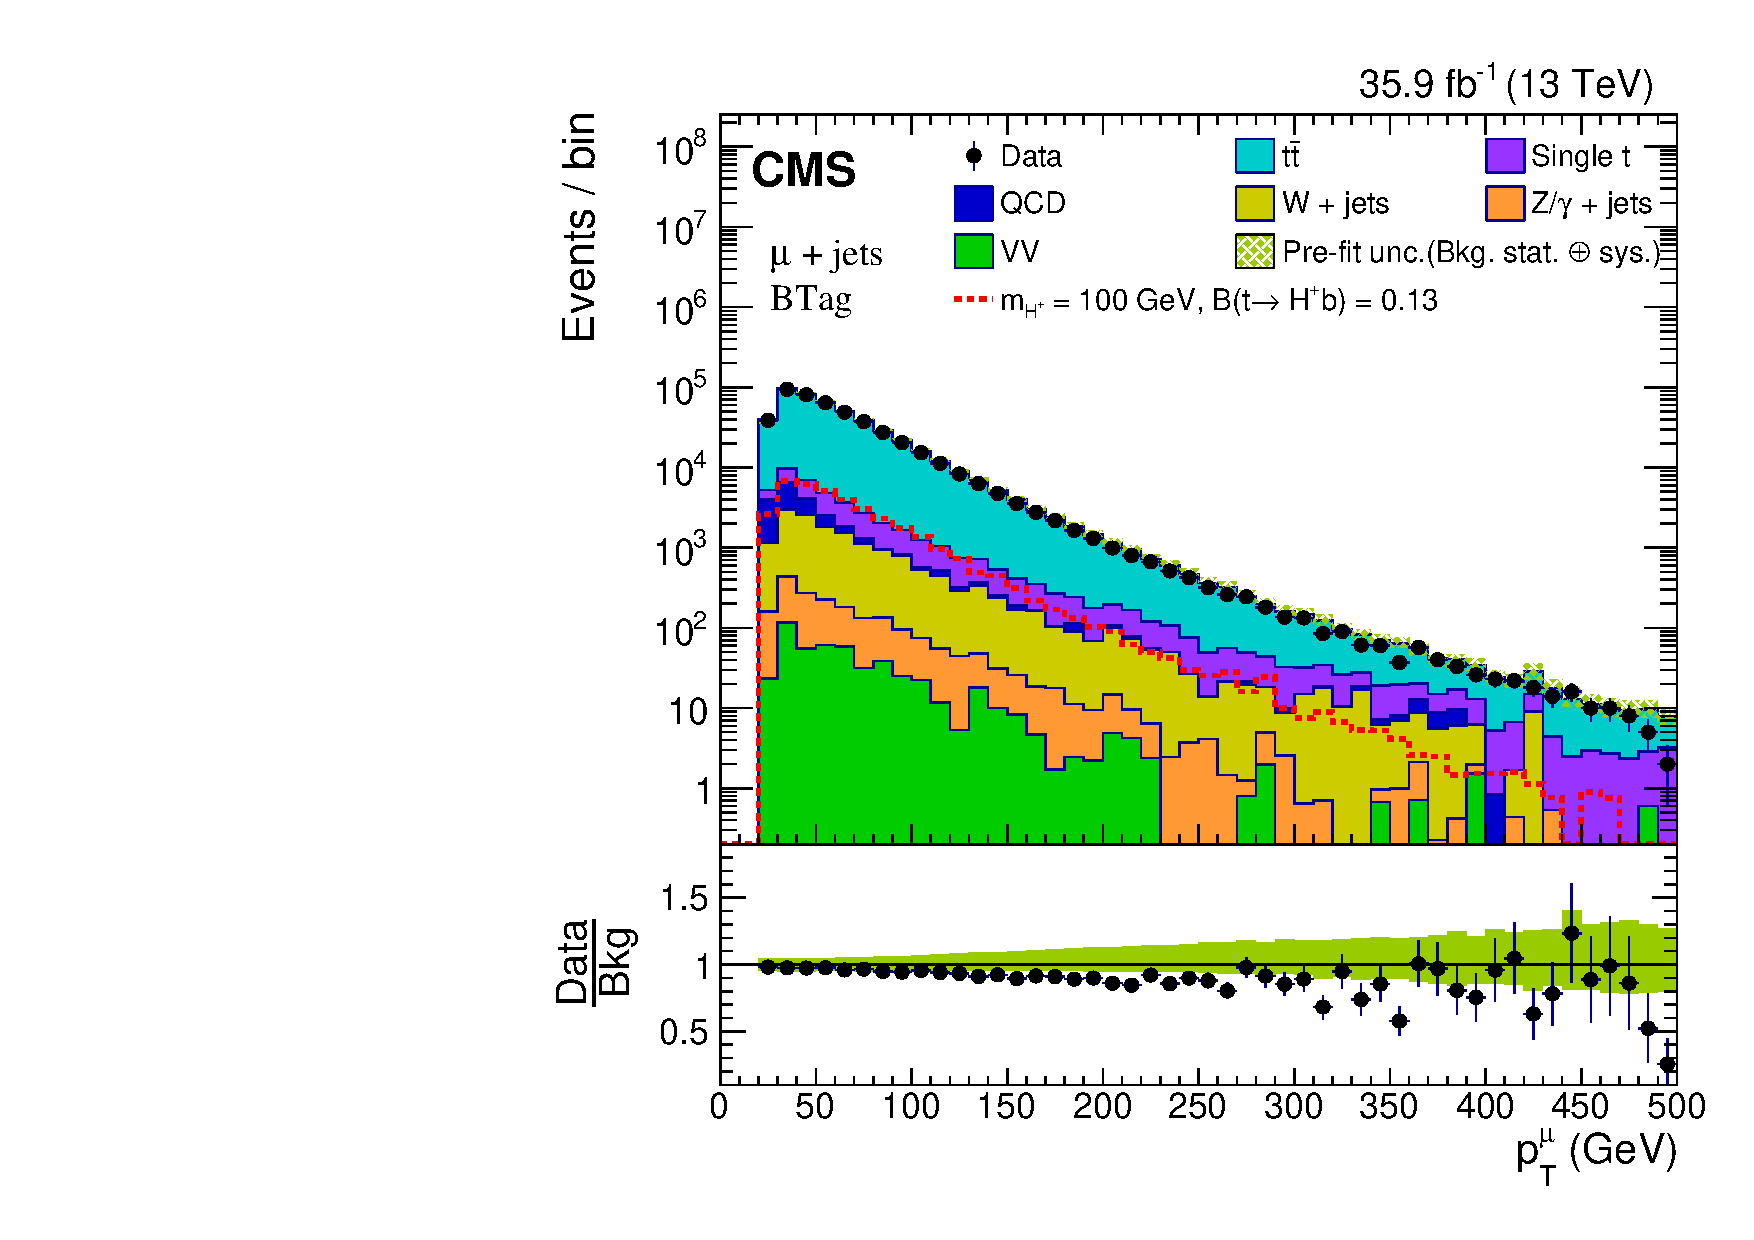
\includegraphics[width=0.45\linewidth]{Image/Muon/BTag/pt_mu_muBTag.pdf}}
    \subfigure[\pt of electrons]{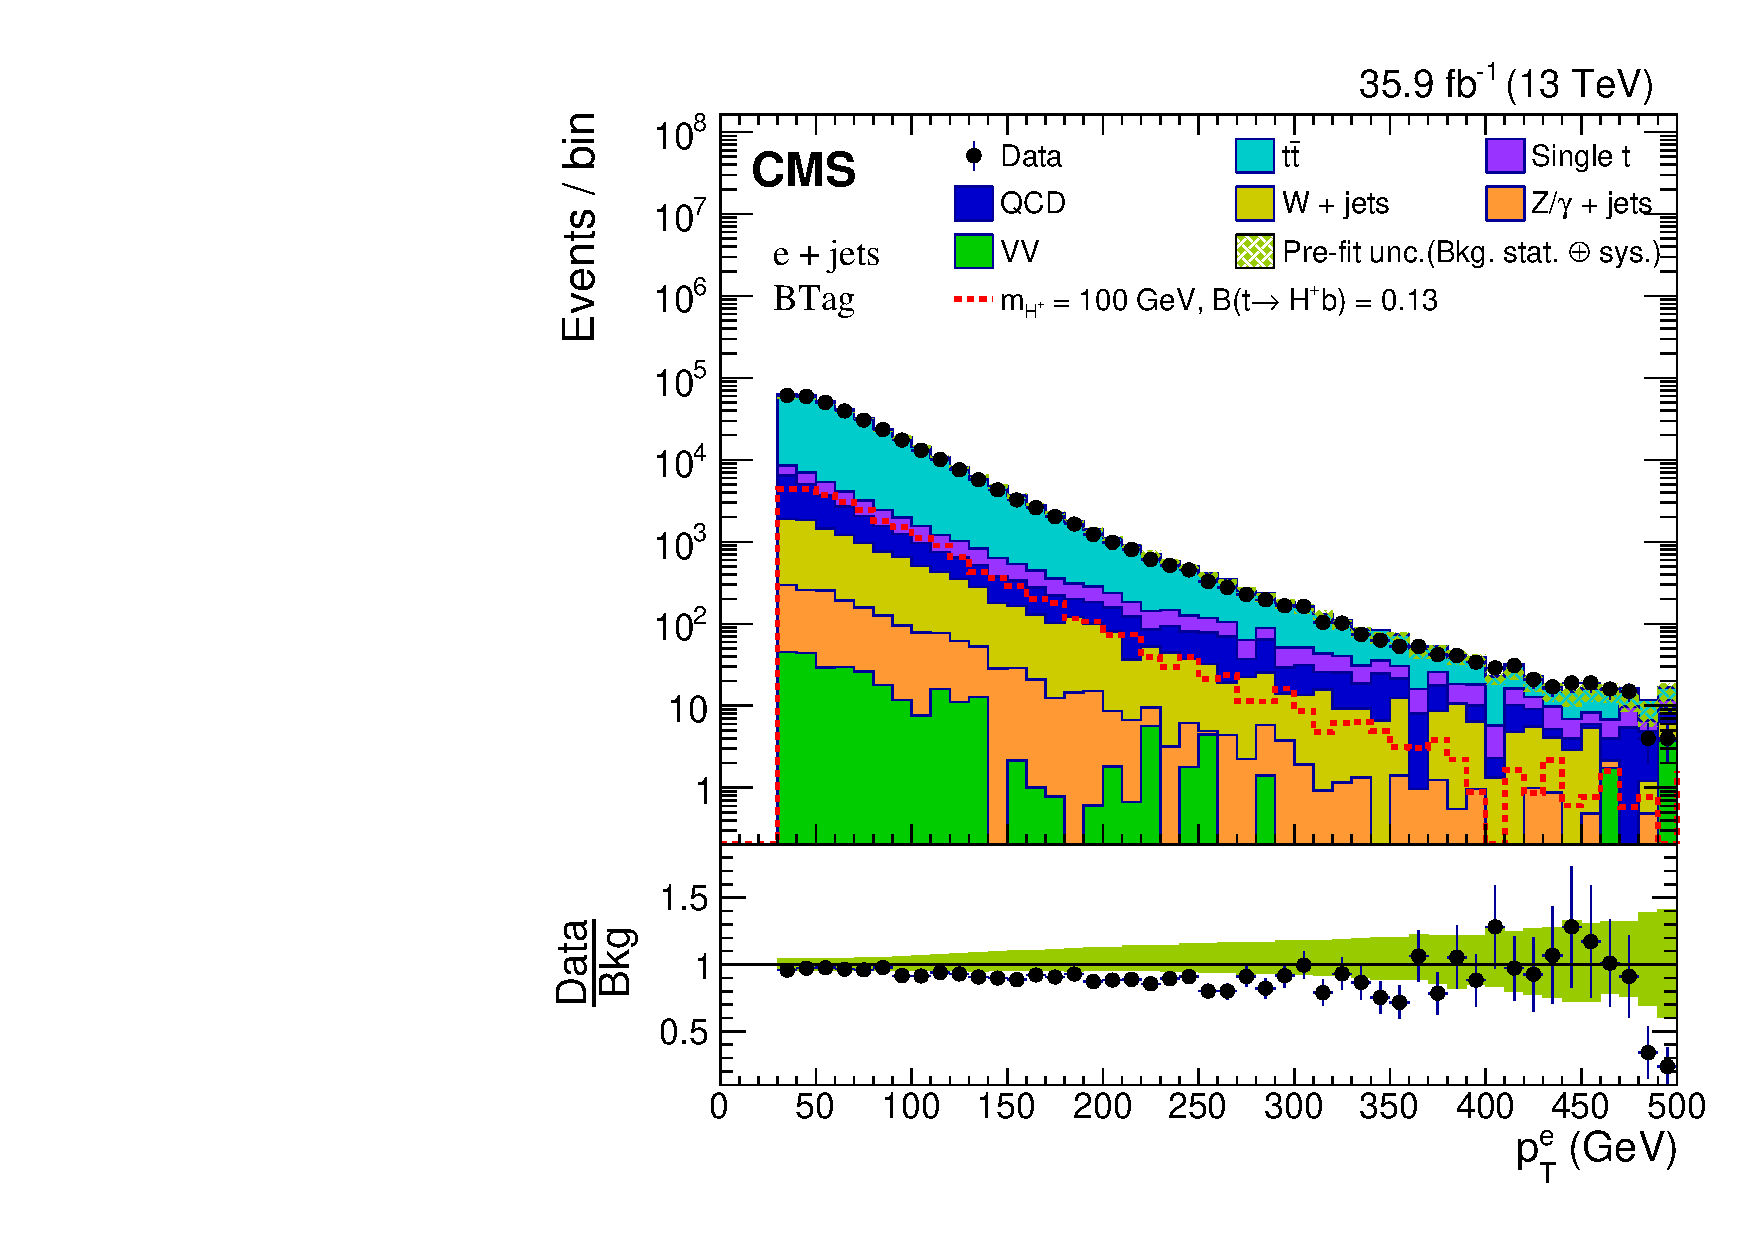
\includegraphics[width=0.45\linewidth]{Image/Electron/BTag/pt_ele_eleBTag.pdf}}
    \vfil
    \subfigure[$\eta$ of muons]{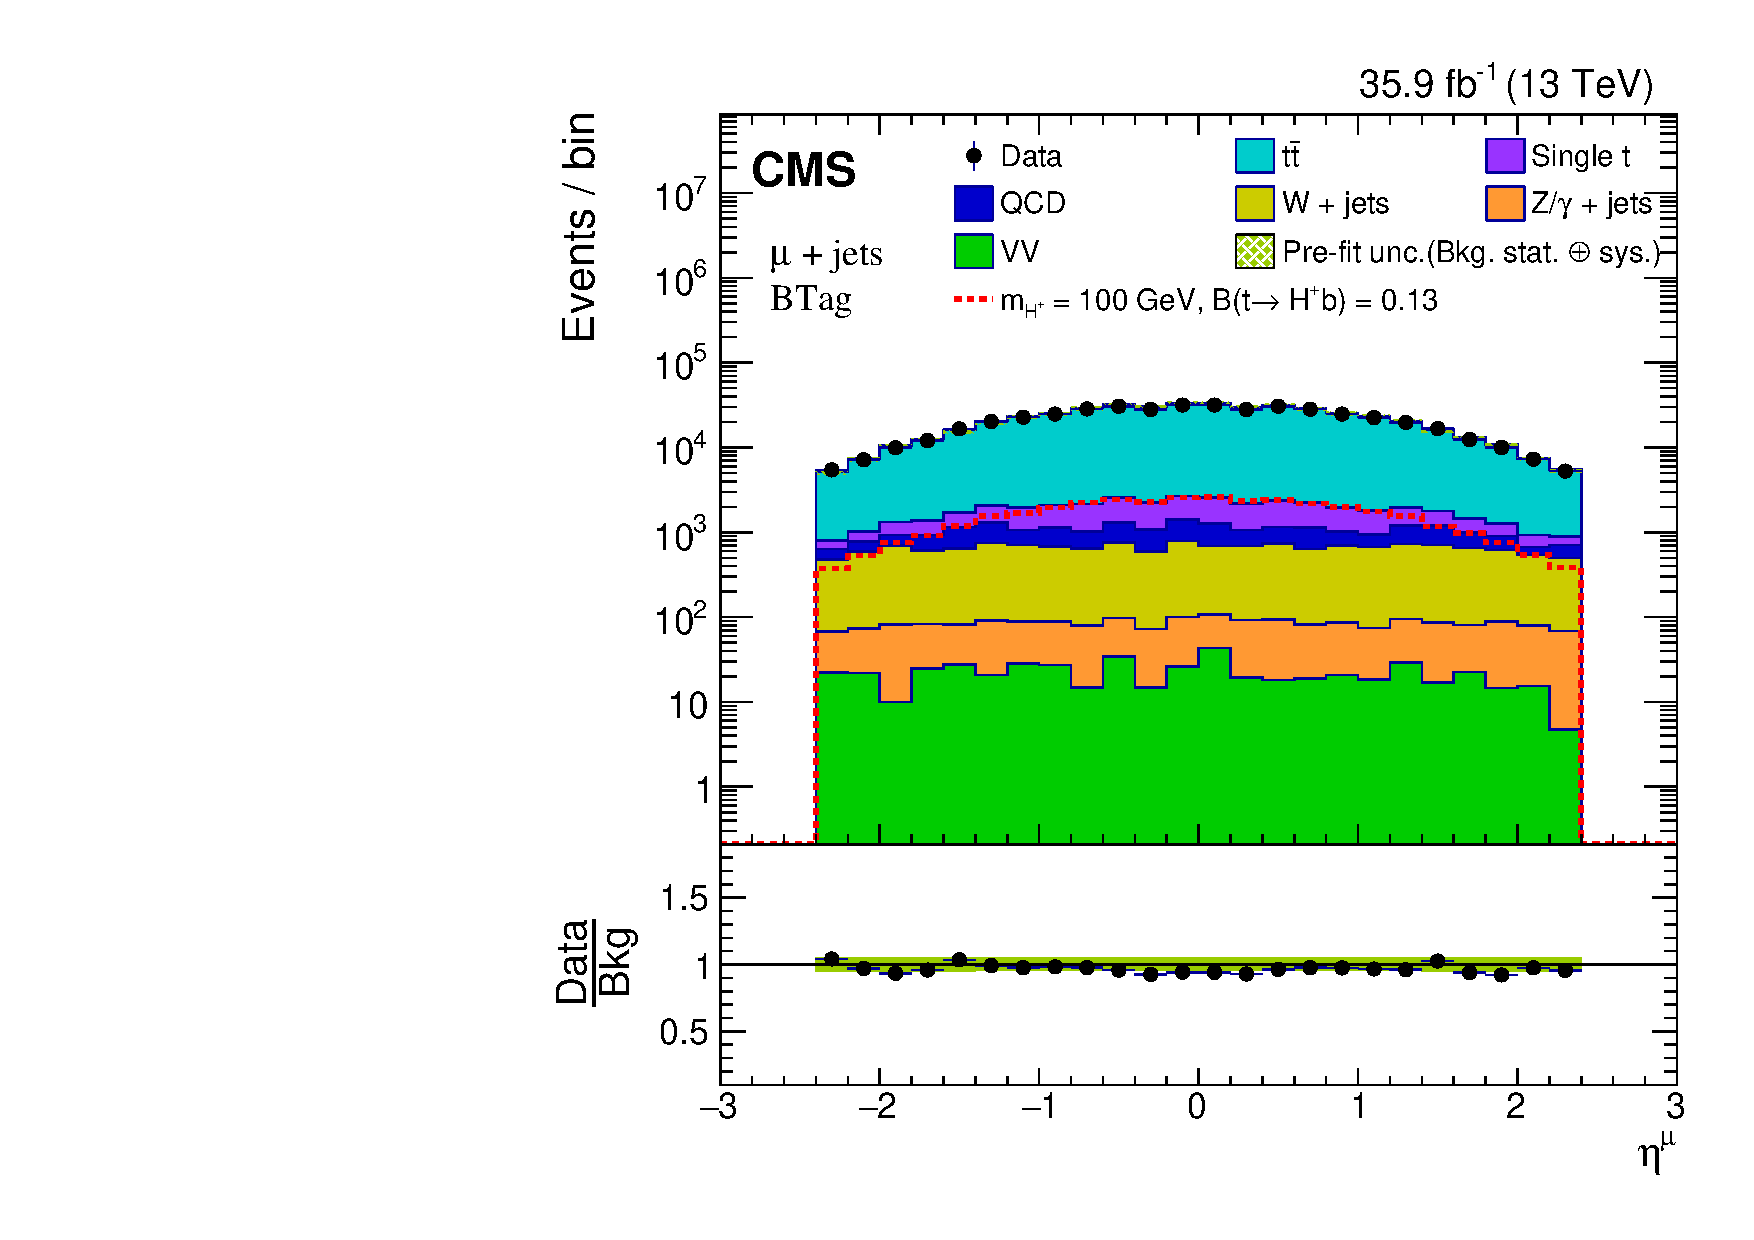
\includegraphics[width=0.45\linewidth]{Image/Muon/BTag/eta_mu_muBTag.pdf}}
    \subfigure[$\eta$ of electrons]{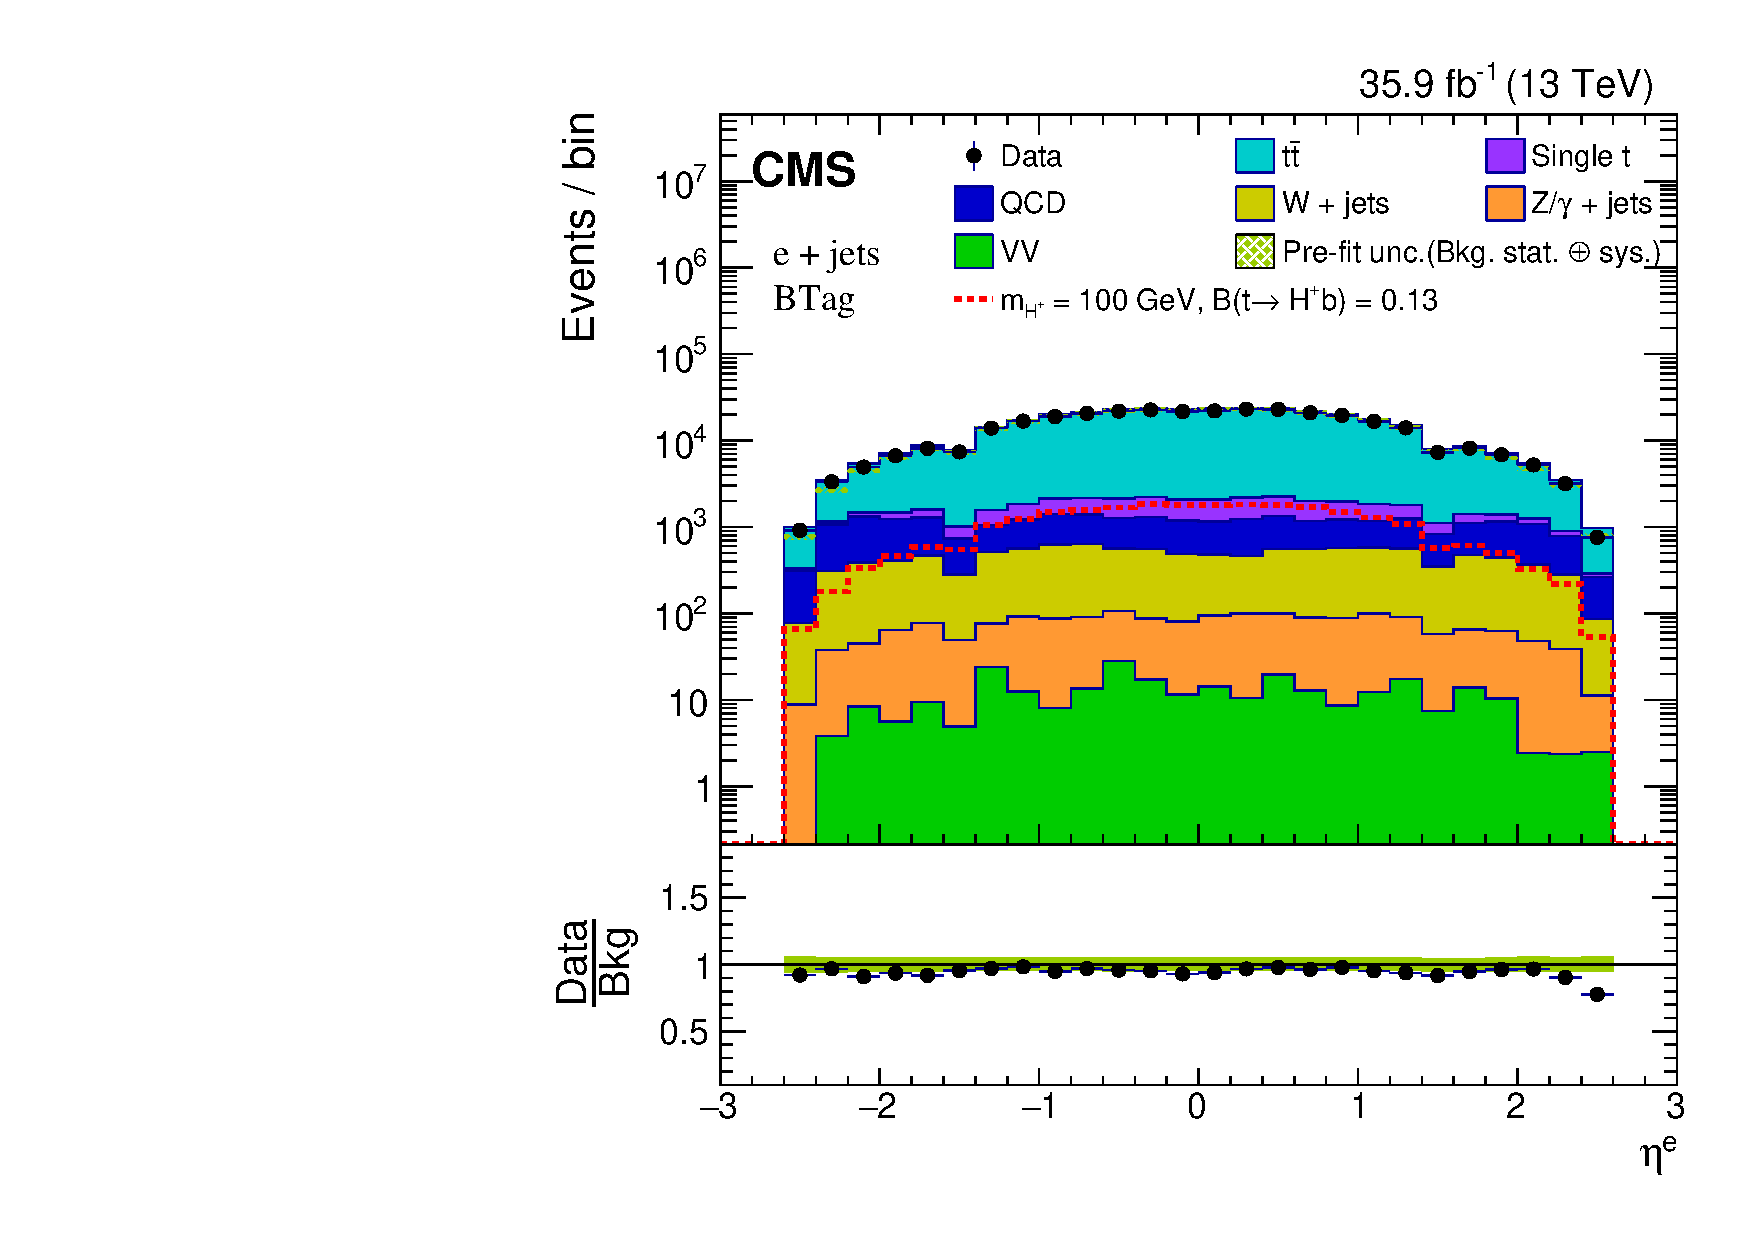
\includegraphics[width=0.45\linewidth]{Image/Electron/BTag/eta_ele_eleBTag.pdf}}
    \vfil
    \subfigure[\pt of jets]{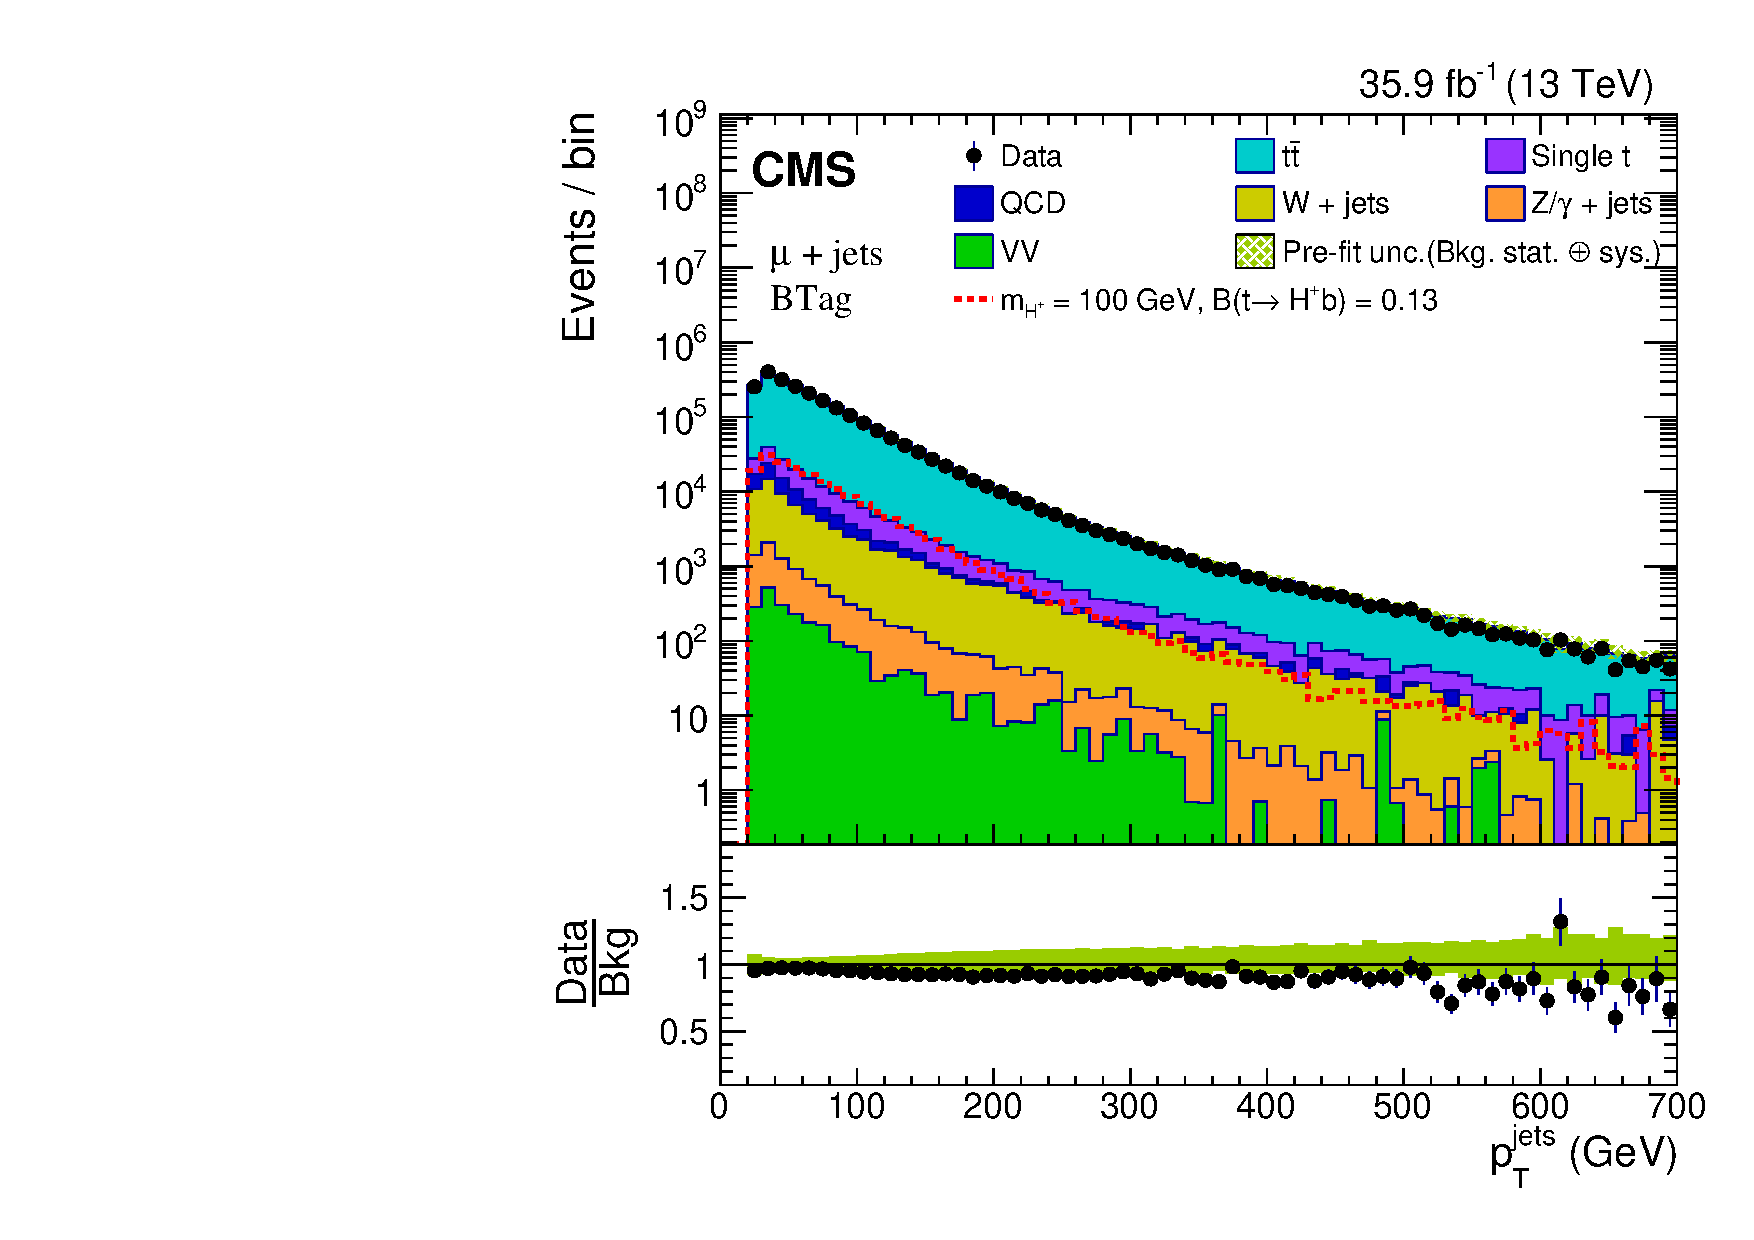
\includegraphics[width=0.45\linewidth]{Image/Muon/BTag/pt_jet_muBTag.pdf}}
    \subfigure[\pt of jets]{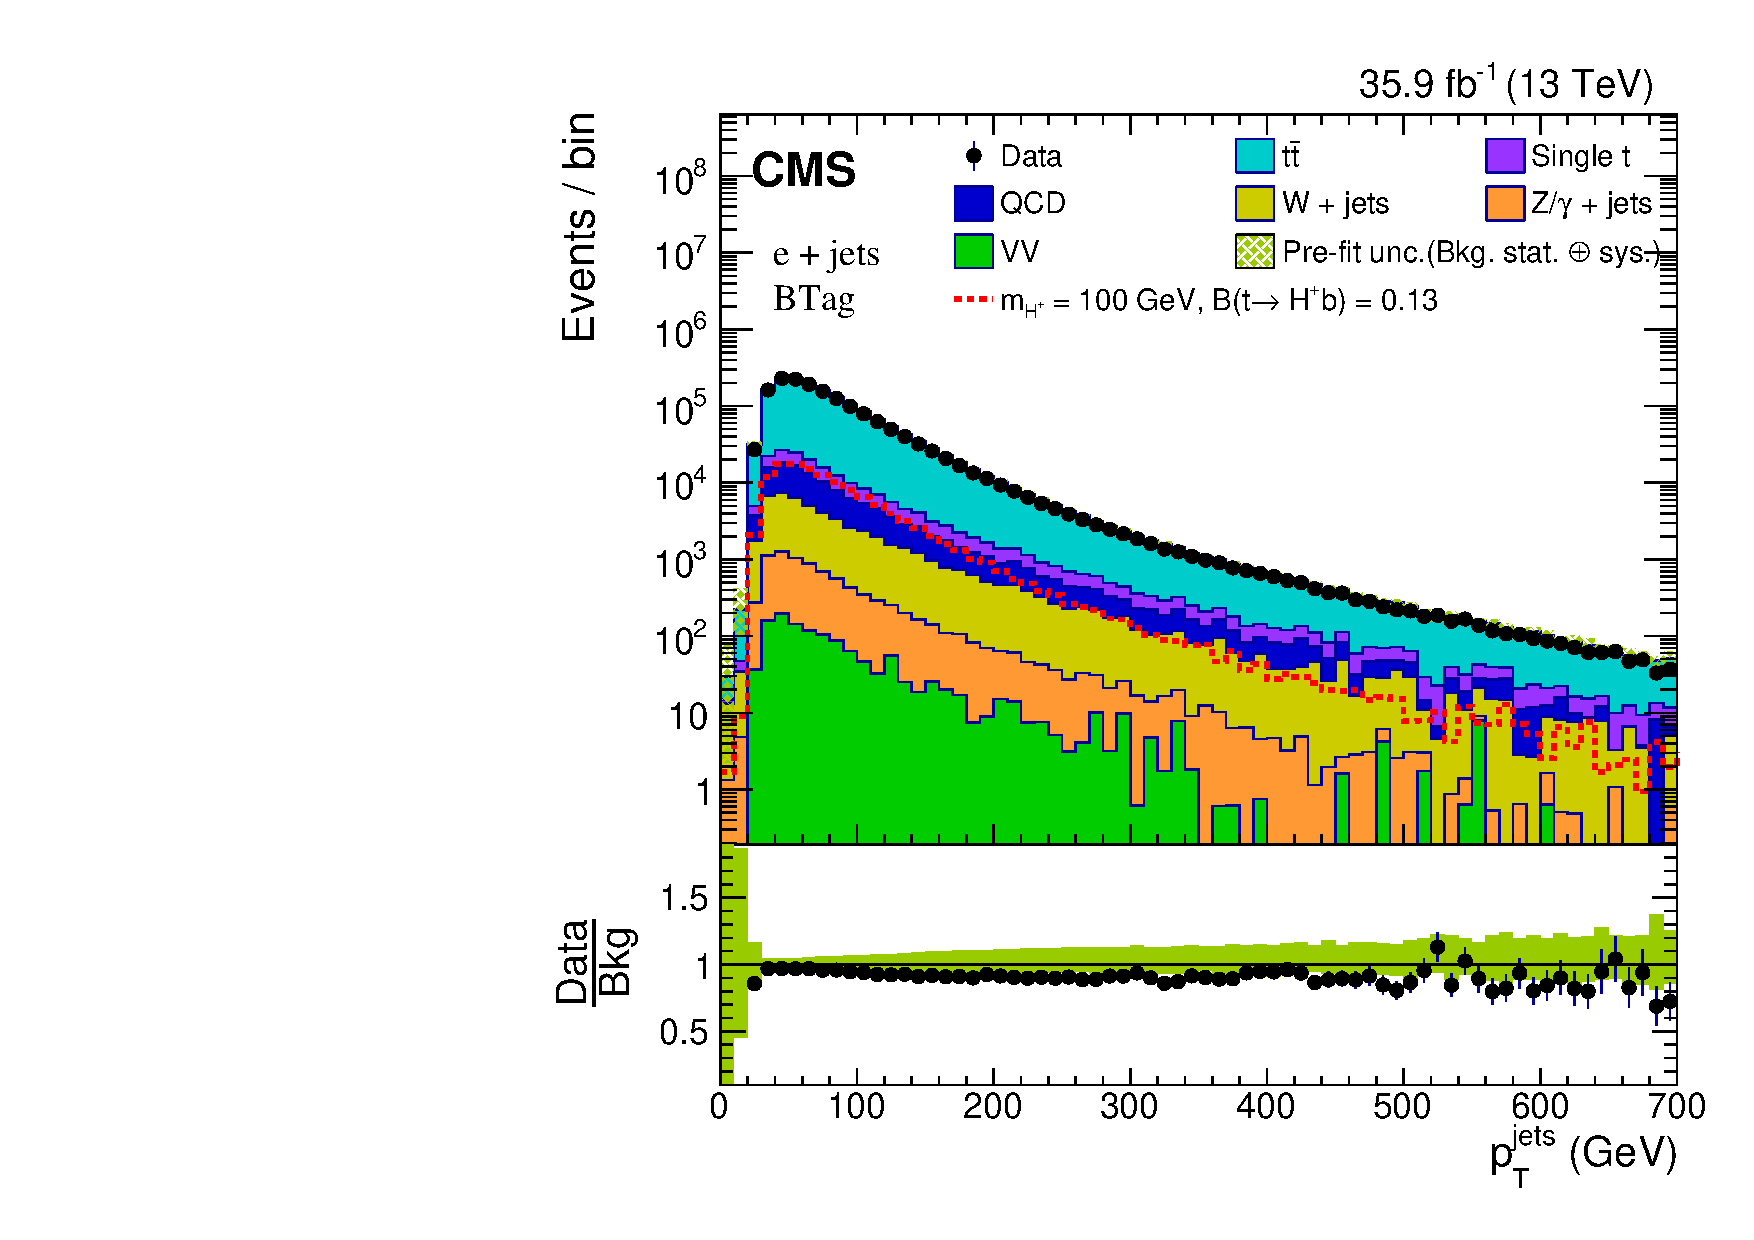
\includegraphics[width=0.45\linewidth]{Image/Electron/BTag/pt_jet_eleBTag.pdf}}
    \caption{Distribution of $\pt, \eta$ of reconstructed lepton and \pt of jets
        after b-jet selection as described in Sec.~\ref{s:secEvtSel}, 
    for muons + jets and \ejets channel.}
    \label{fig:btagPlot1}
\end{figure}

%After BTagging: Eta_jets, N_jets, N_bjets
\begin{figure}
    \centering  
    \subfigure[$\eta$ of jets]{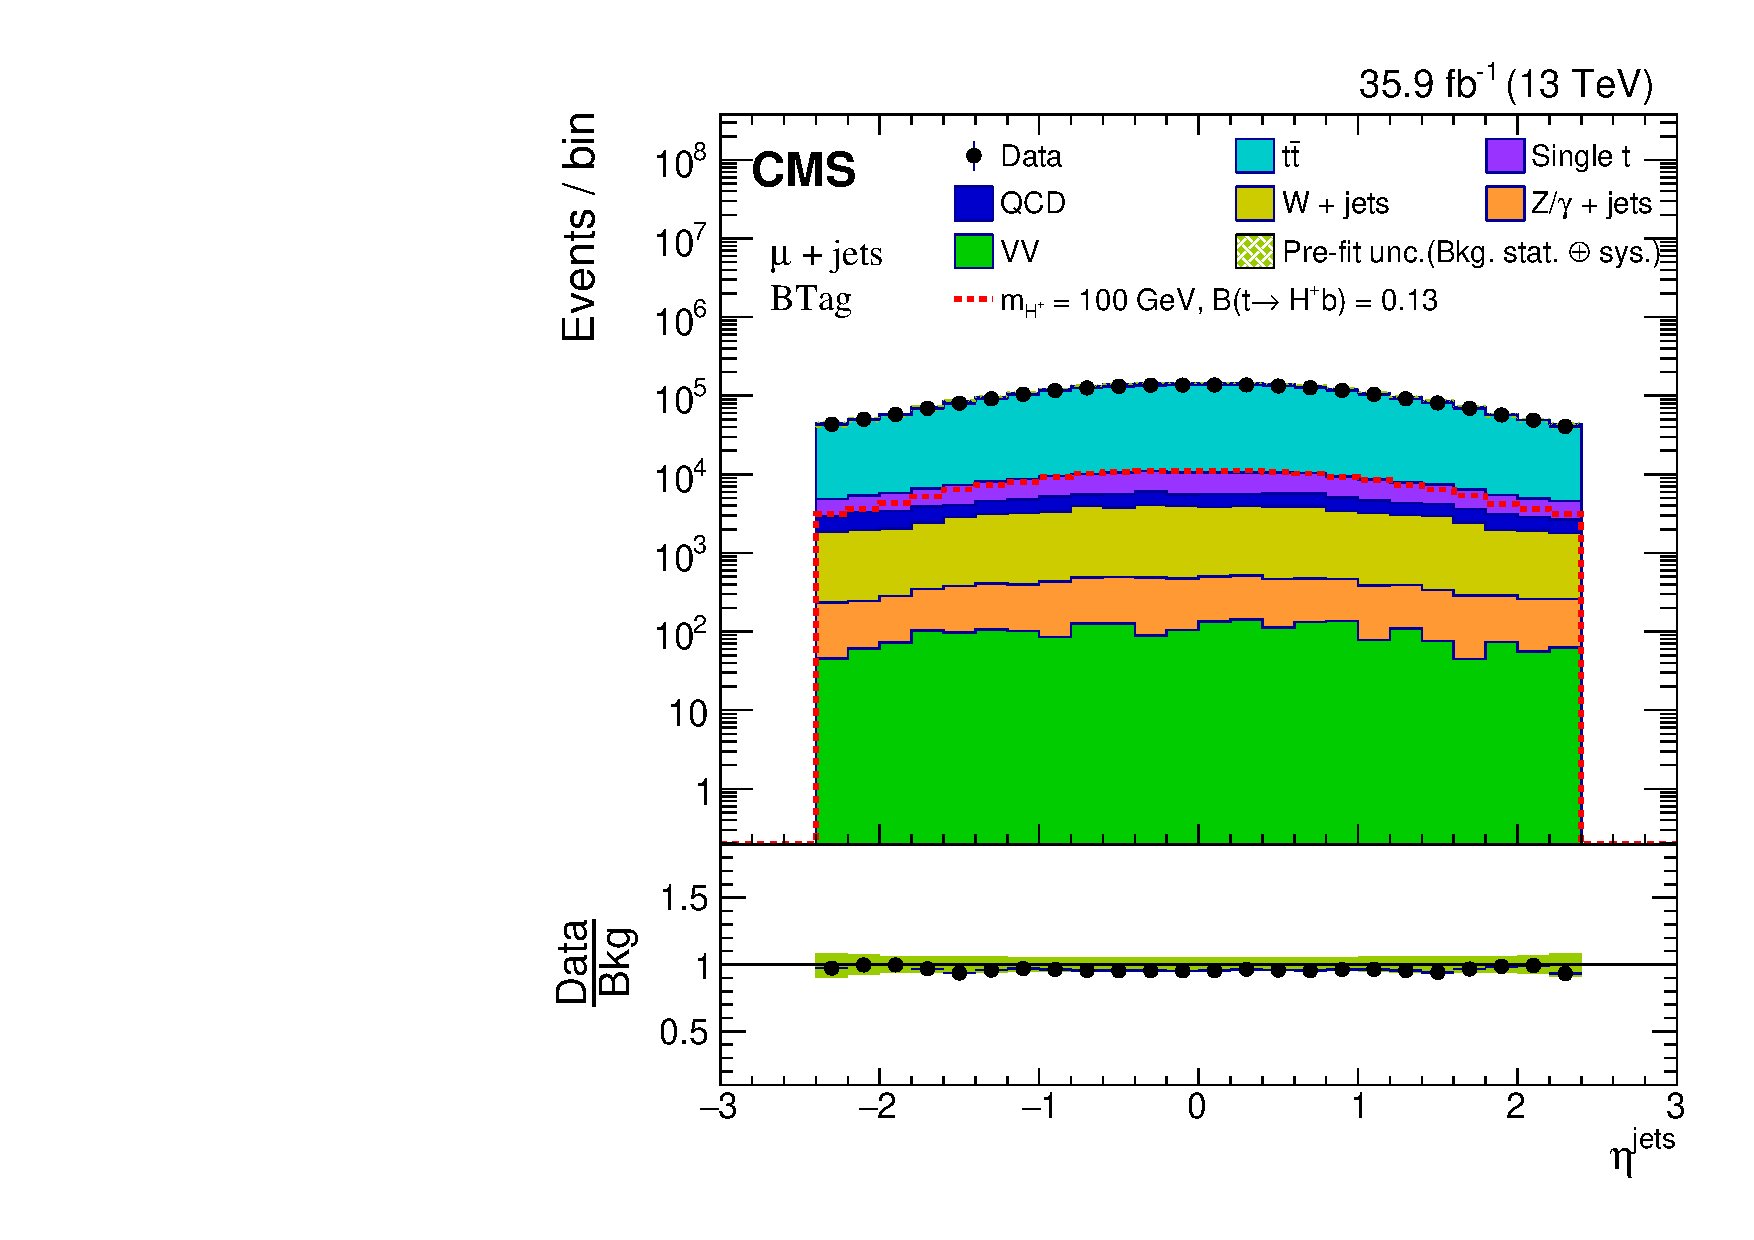
\includegraphics[width=0.45\linewidth]{Image/Muon/BTag/eta_jet_muBTag.pdf}}
    \subfigure[$\eta$ of jets]{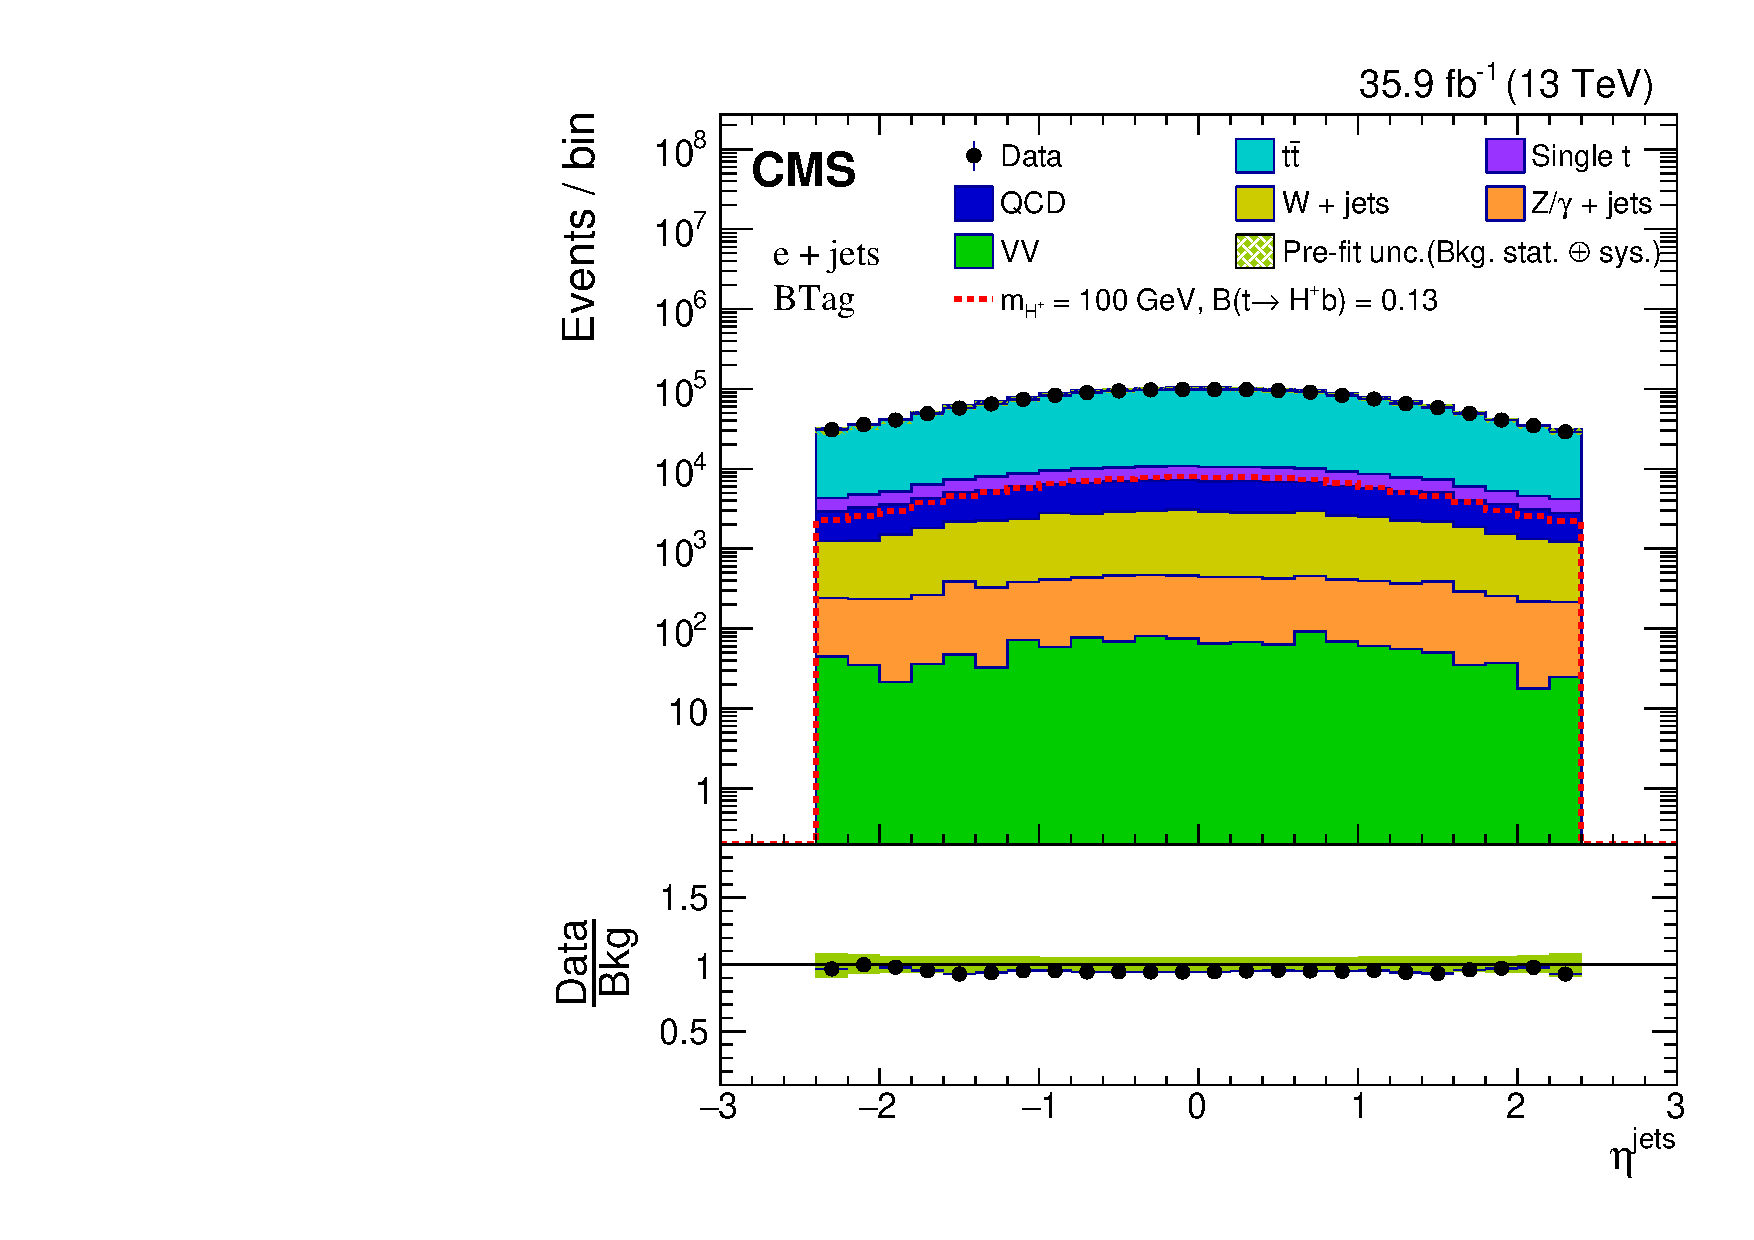
\includegraphics[width=0.45\linewidth]{Image/Electron/BTag/eta_jet_eleBTag.pdf}}
    \vfil
    \subfigure[jet multiplicity]{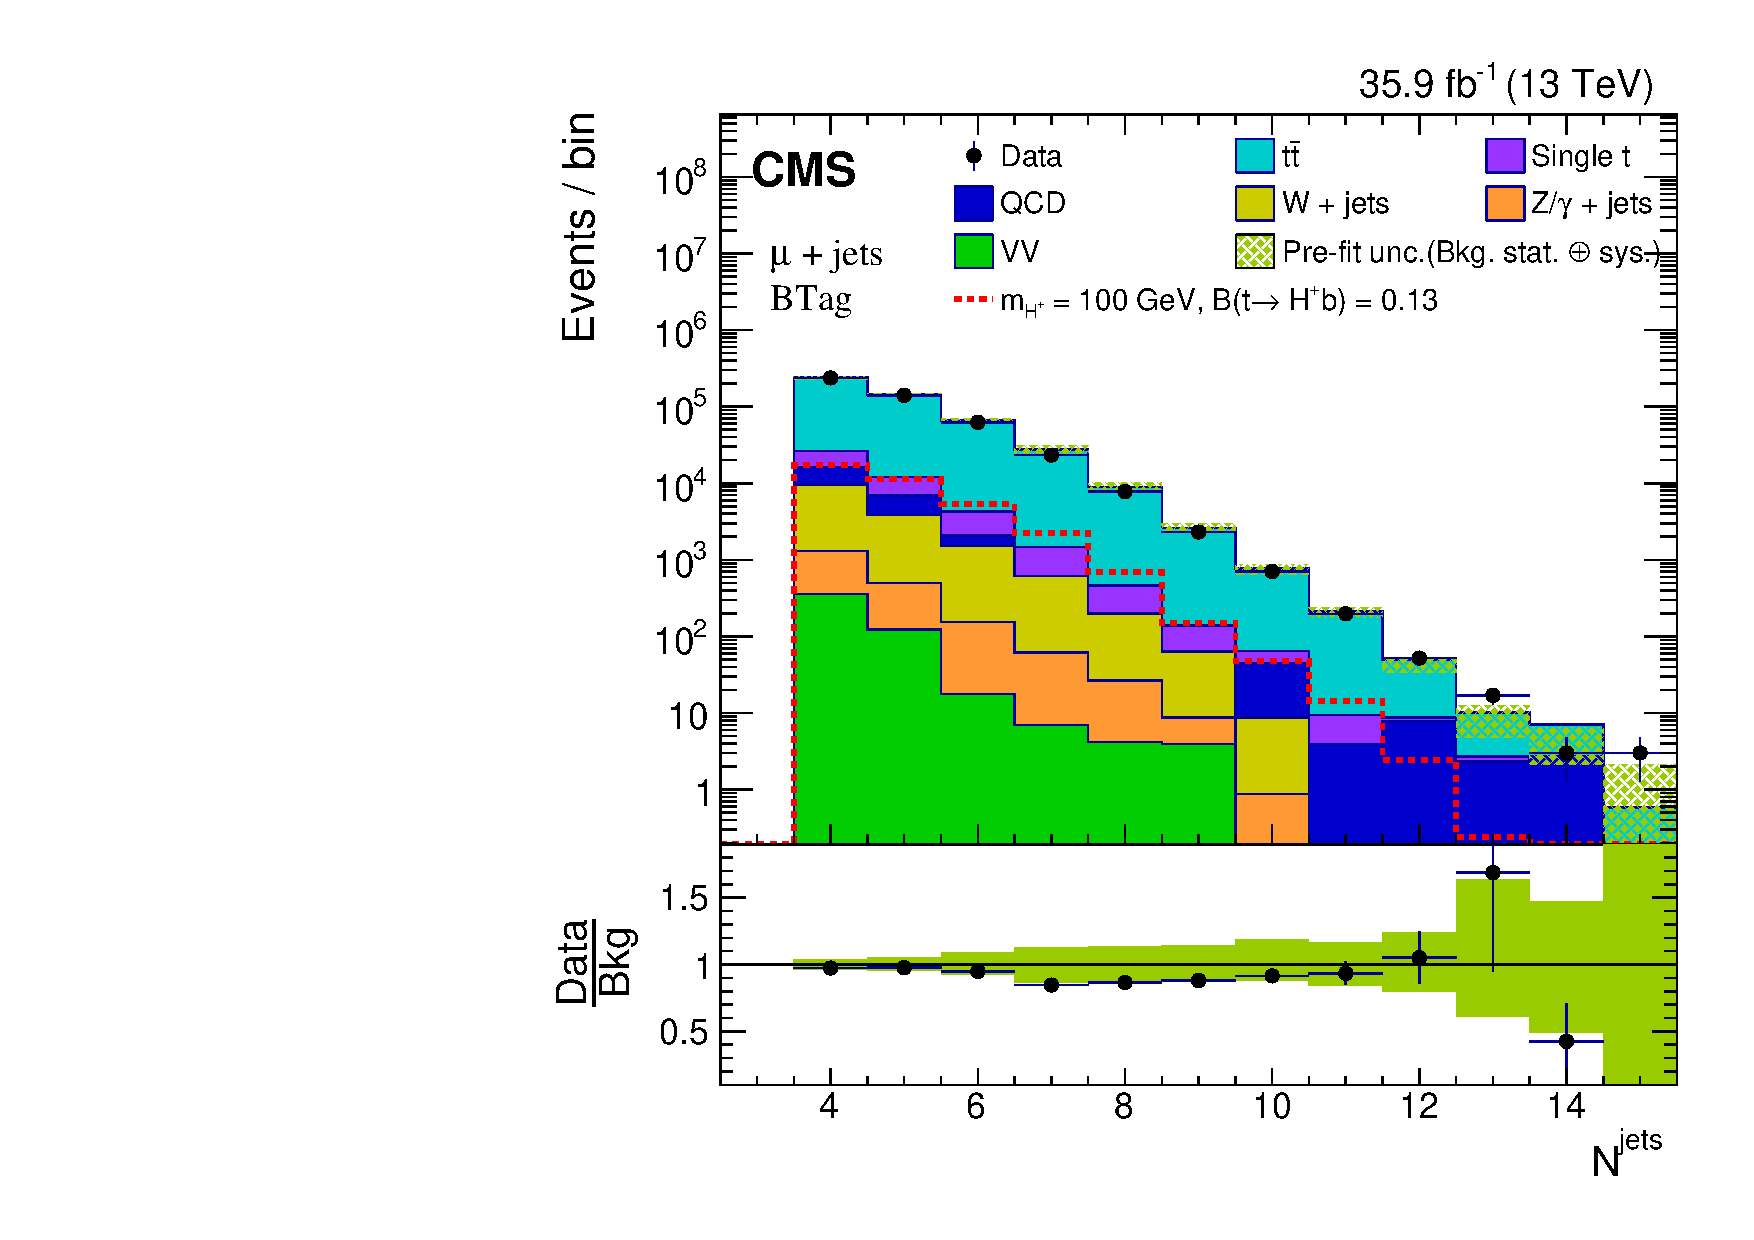
\includegraphics[width=0.45\linewidth]{Image/Muon/BTag/final_multi_jet_muBTag.pdf}}
    \subfigure[jet multiplicity]{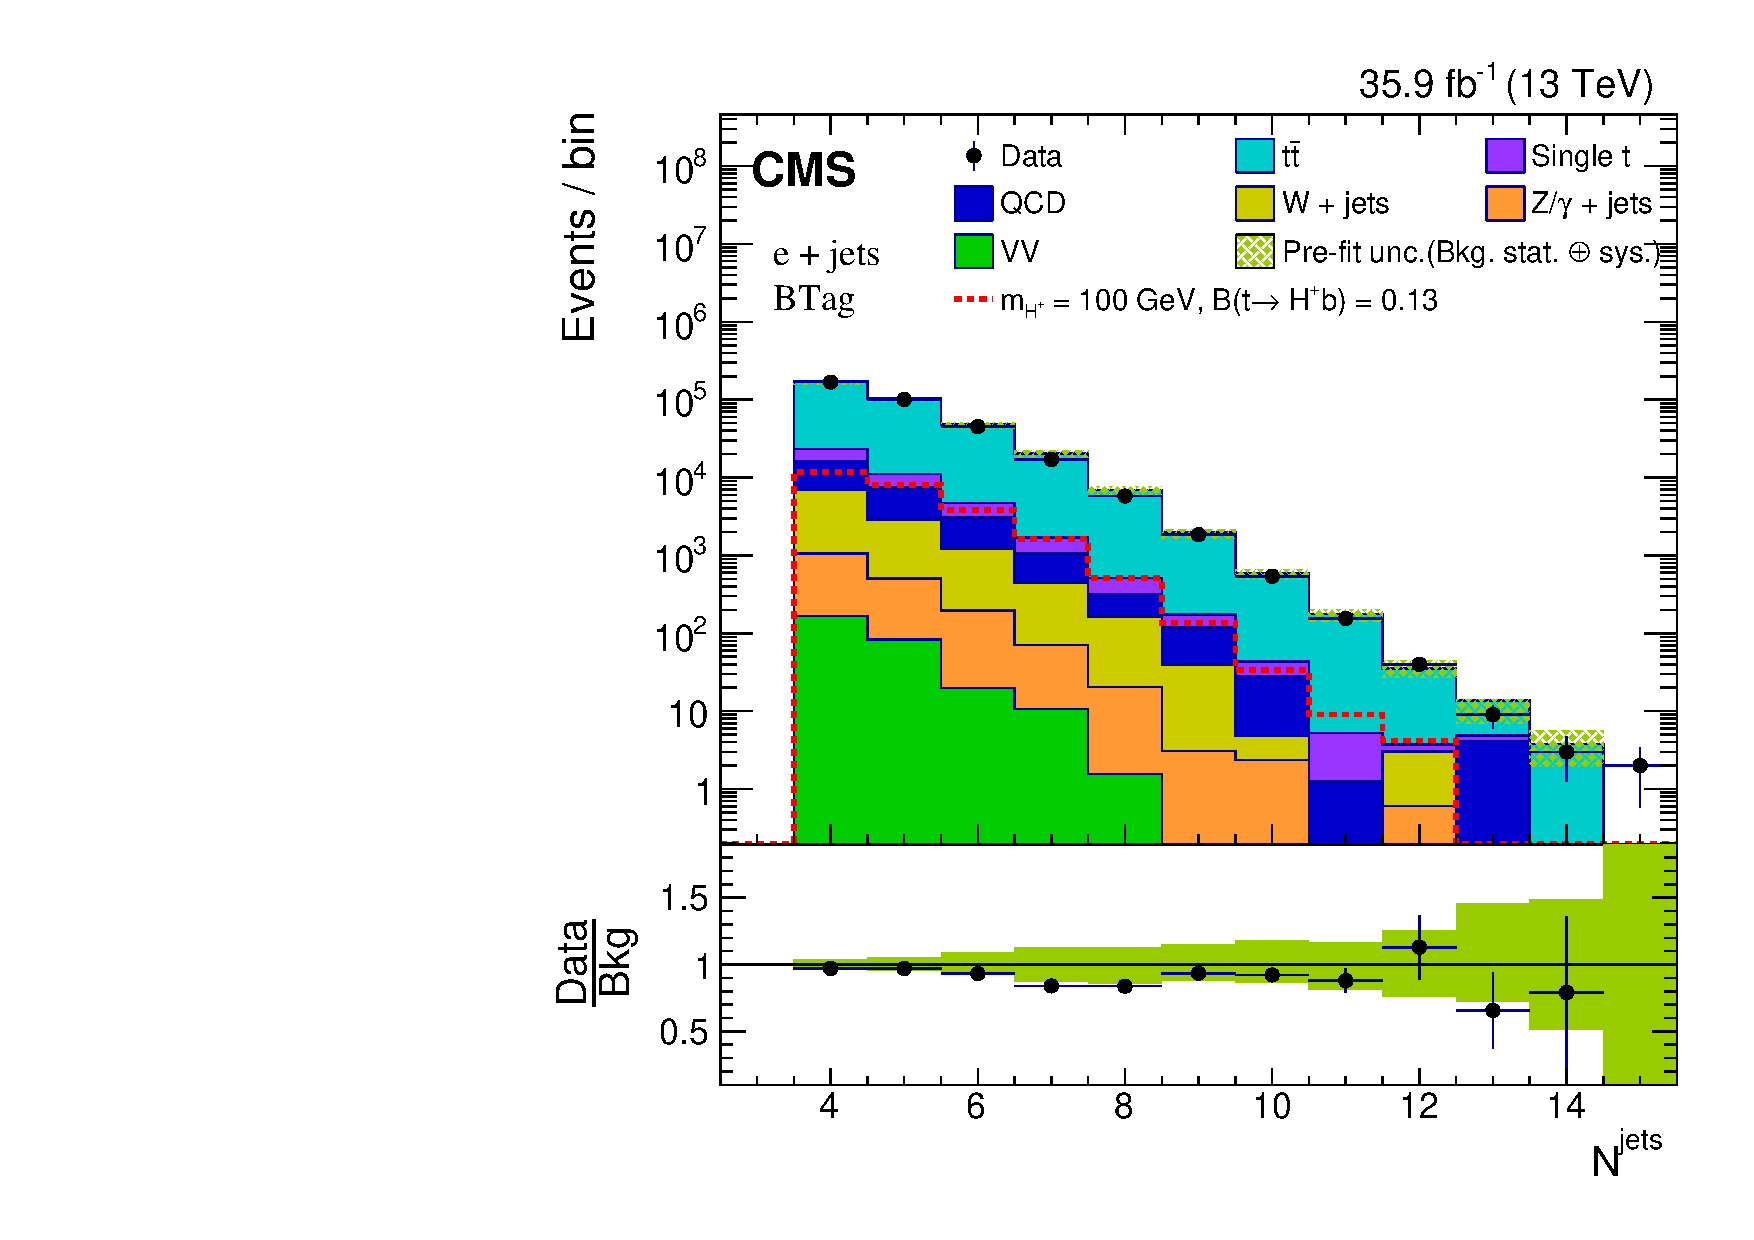
\includegraphics[width=0.45\linewidth]{Image/Electron/BTag/final_multi_jet_eleBTag.pdf}}
    \vfil
    \subfigure[b-jet multiplicity]{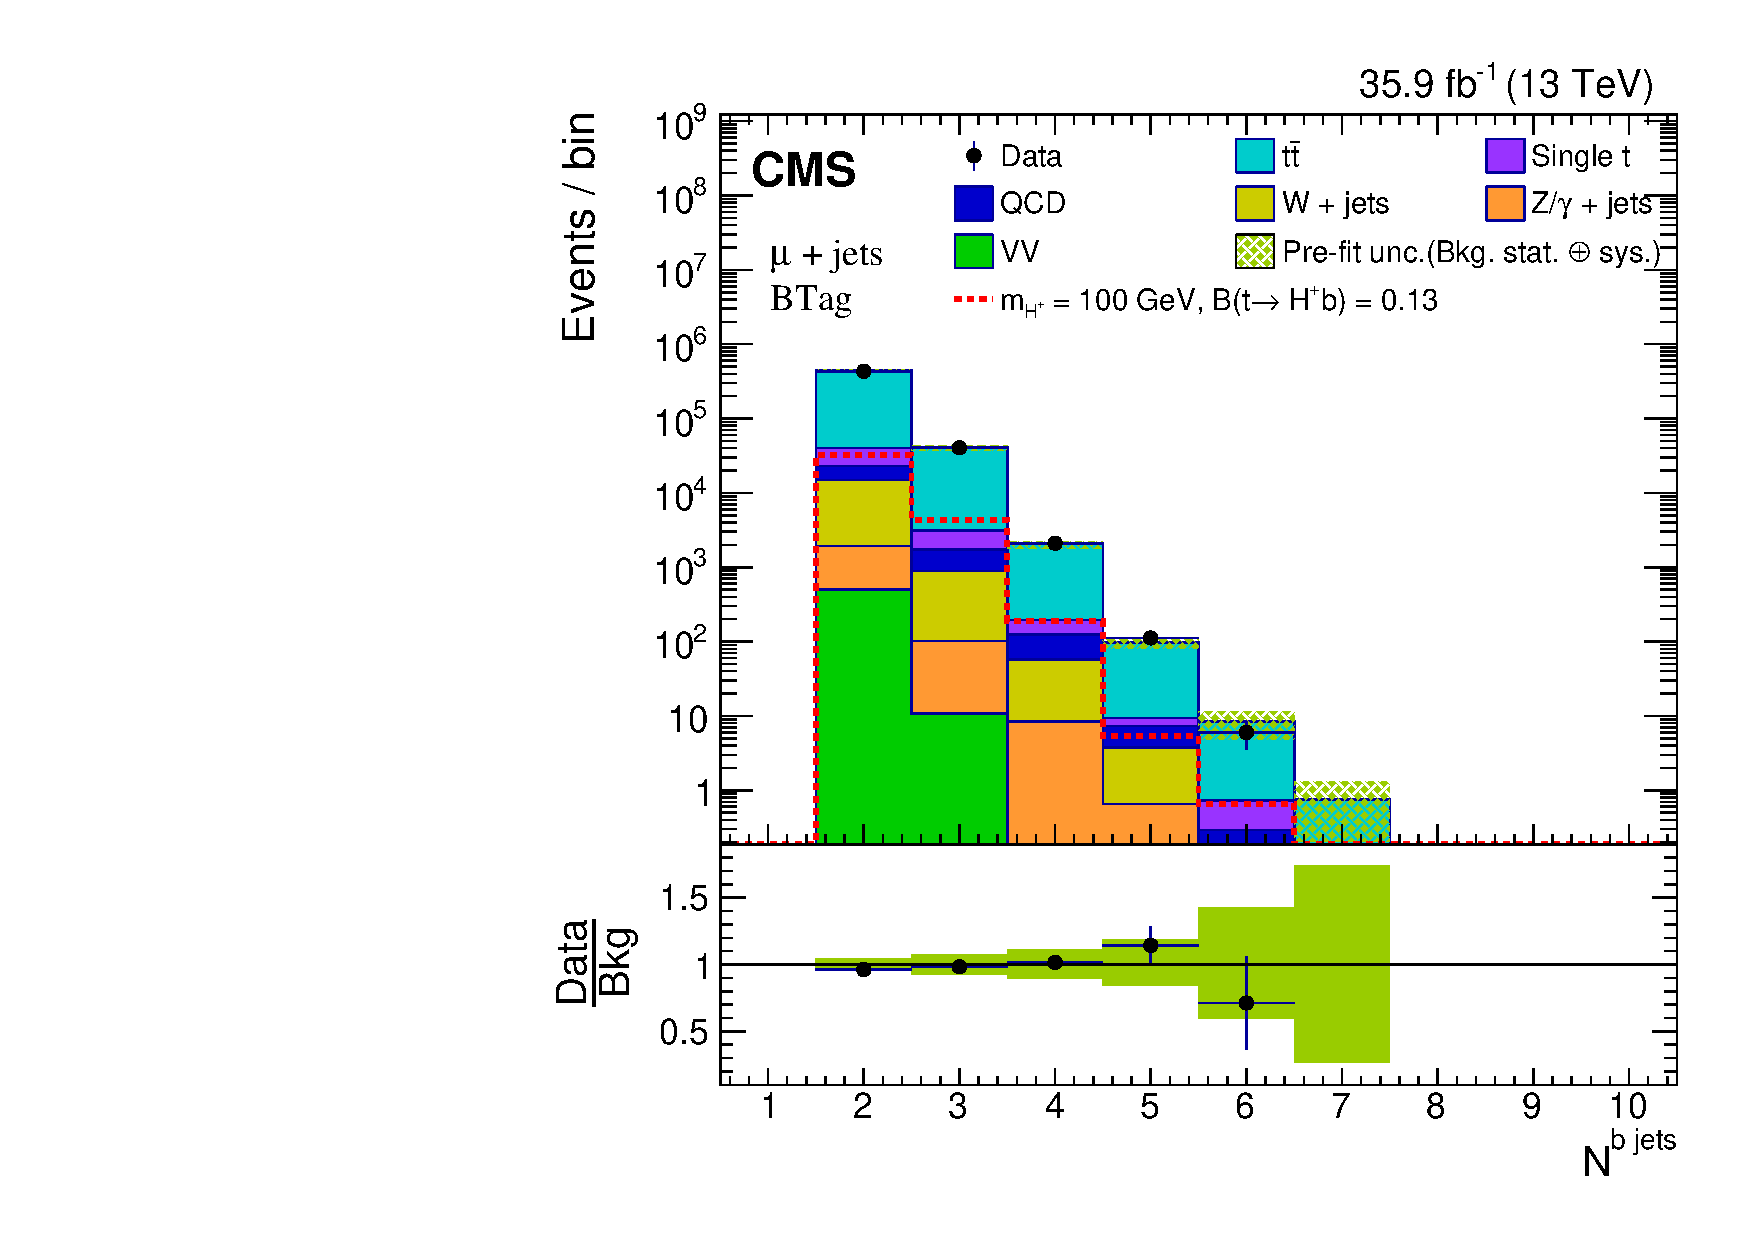
\includegraphics[width=0.45\linewidth]{Image/Muon/BTag/CSVL_count_muBTag.pdf}}
    \subfigure[b-jet multiplicity]{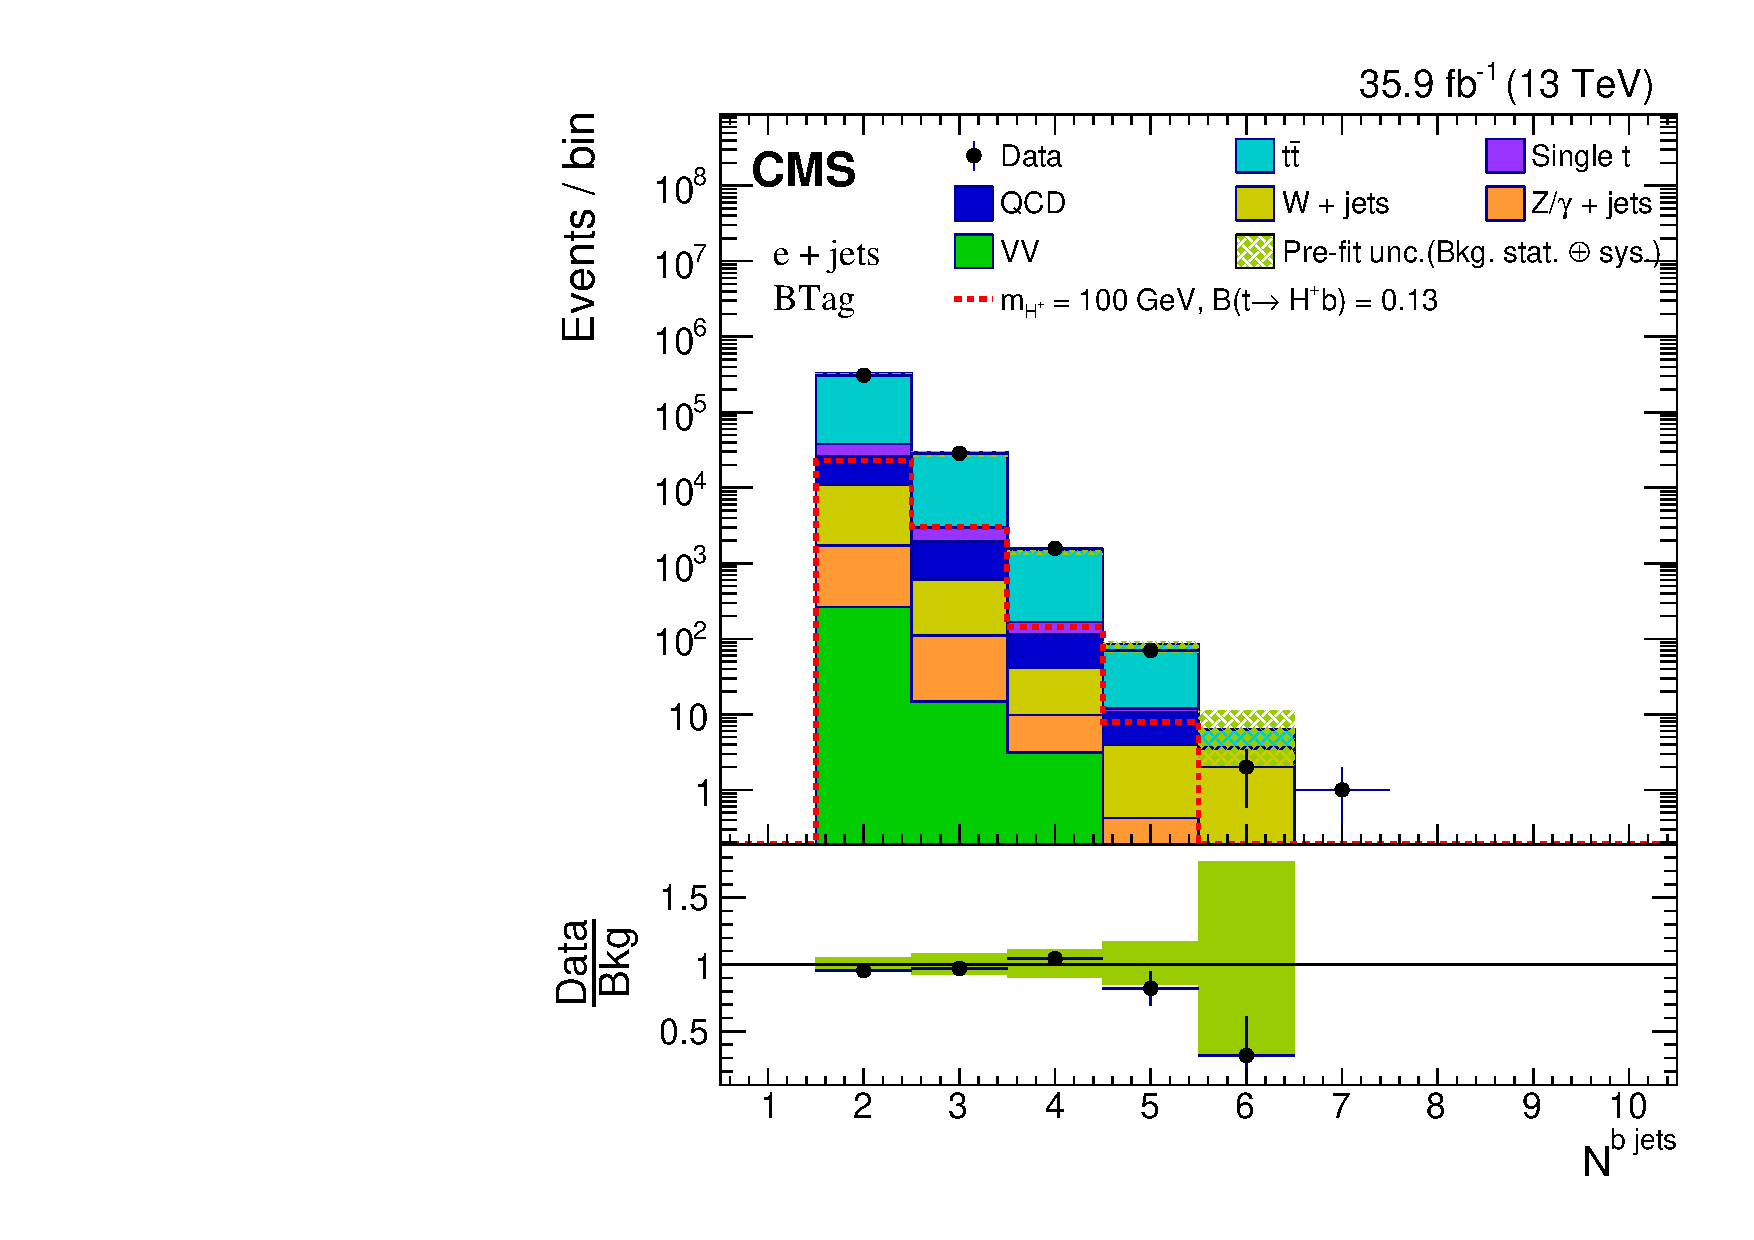
\includegraphics[width=0.45\linewidth]{Image/Electron/BTag/CSVL_count_eleBTag.pdf}}
    \caption{Distribution of reconstructed $\eta$ of jets, jet-multiplicity, and 
        b-jet multiplicity after b-jet selection as described in 
        Sec.~\ref{s:secEvtSel}, for muons + jets and \ejets channel.}
    \label{fig:btagPlot2}
\end{figure}

%After BTagging: \MET, MT 
\begin{figure}
    \centering  
    \subfigure[\MET]{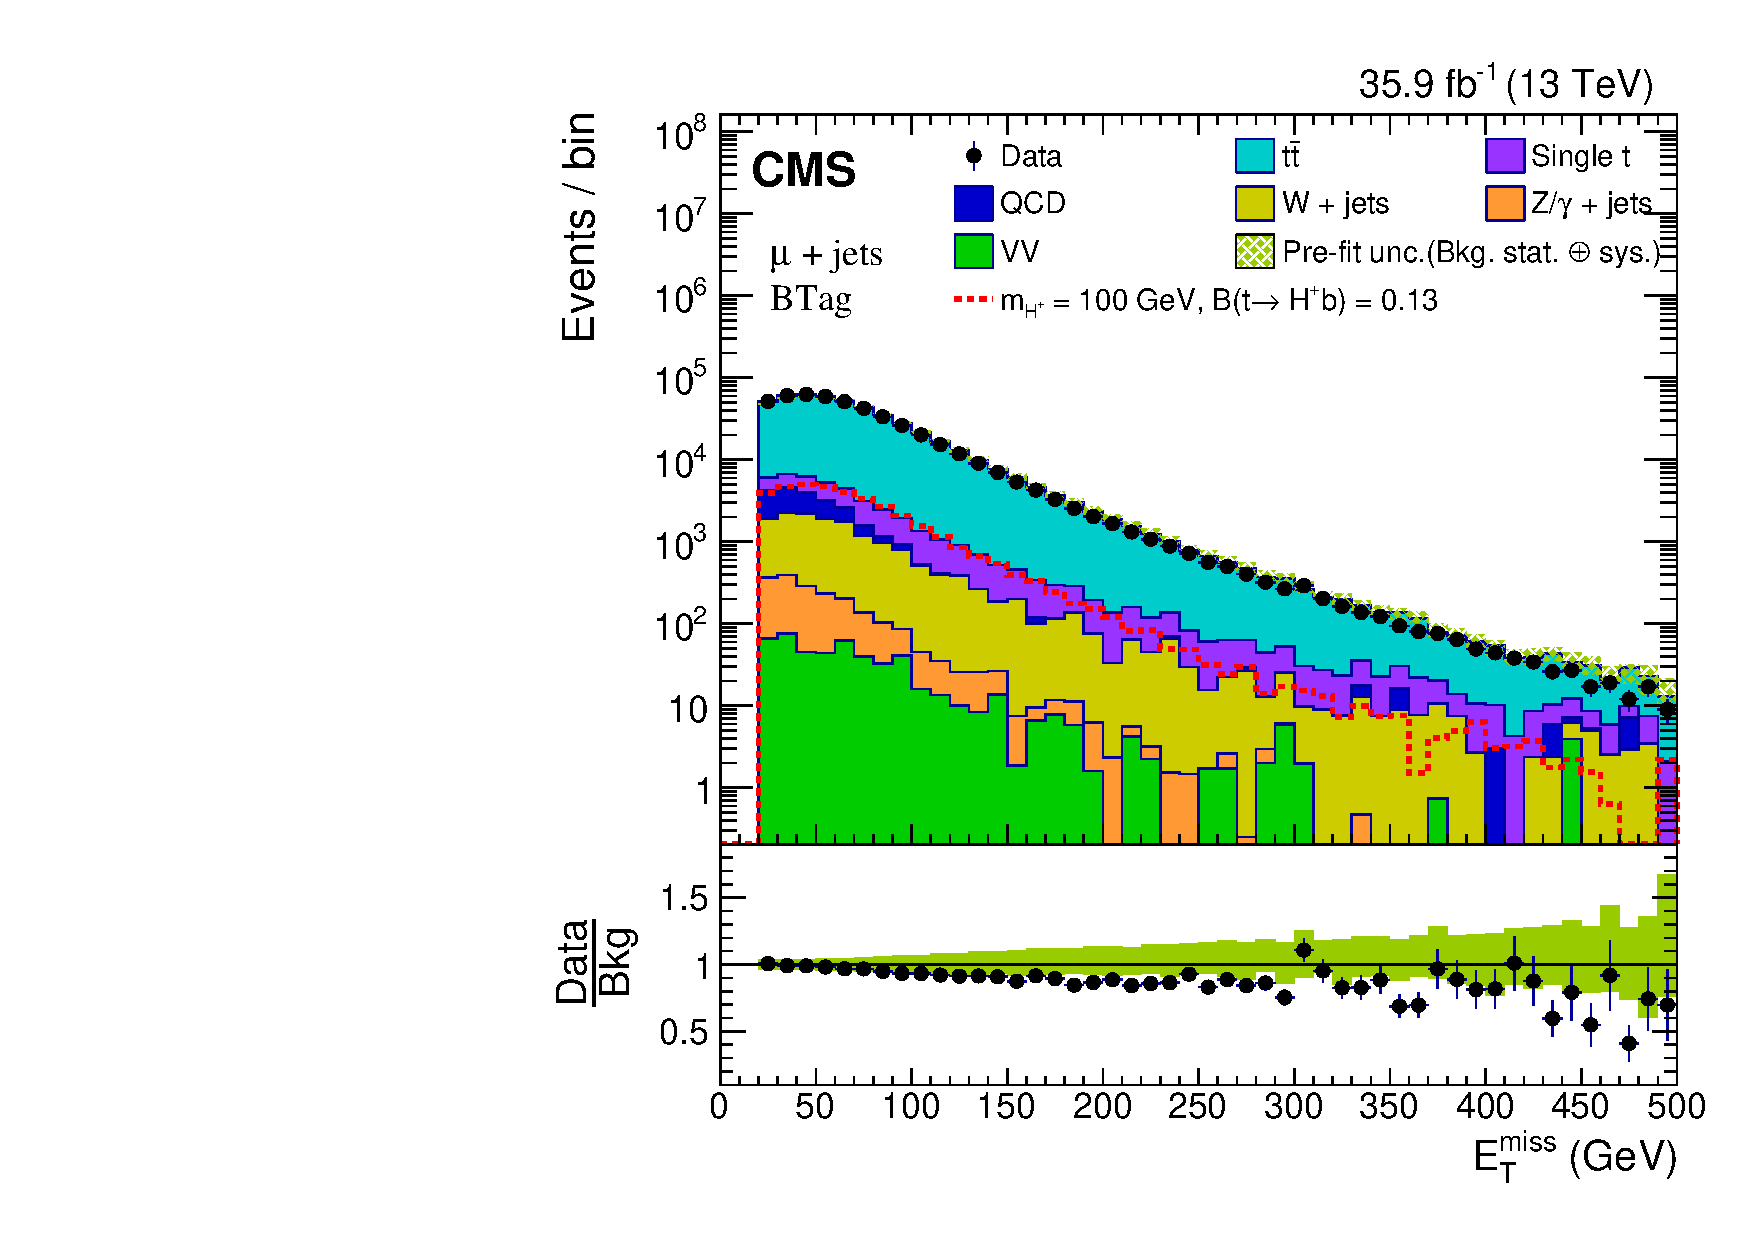
\includegraphics[width=0.45\linewidth]{Image/Muon/BTag/final_pt_met_muBTag.pdf}}
    \subfigure[\MET]{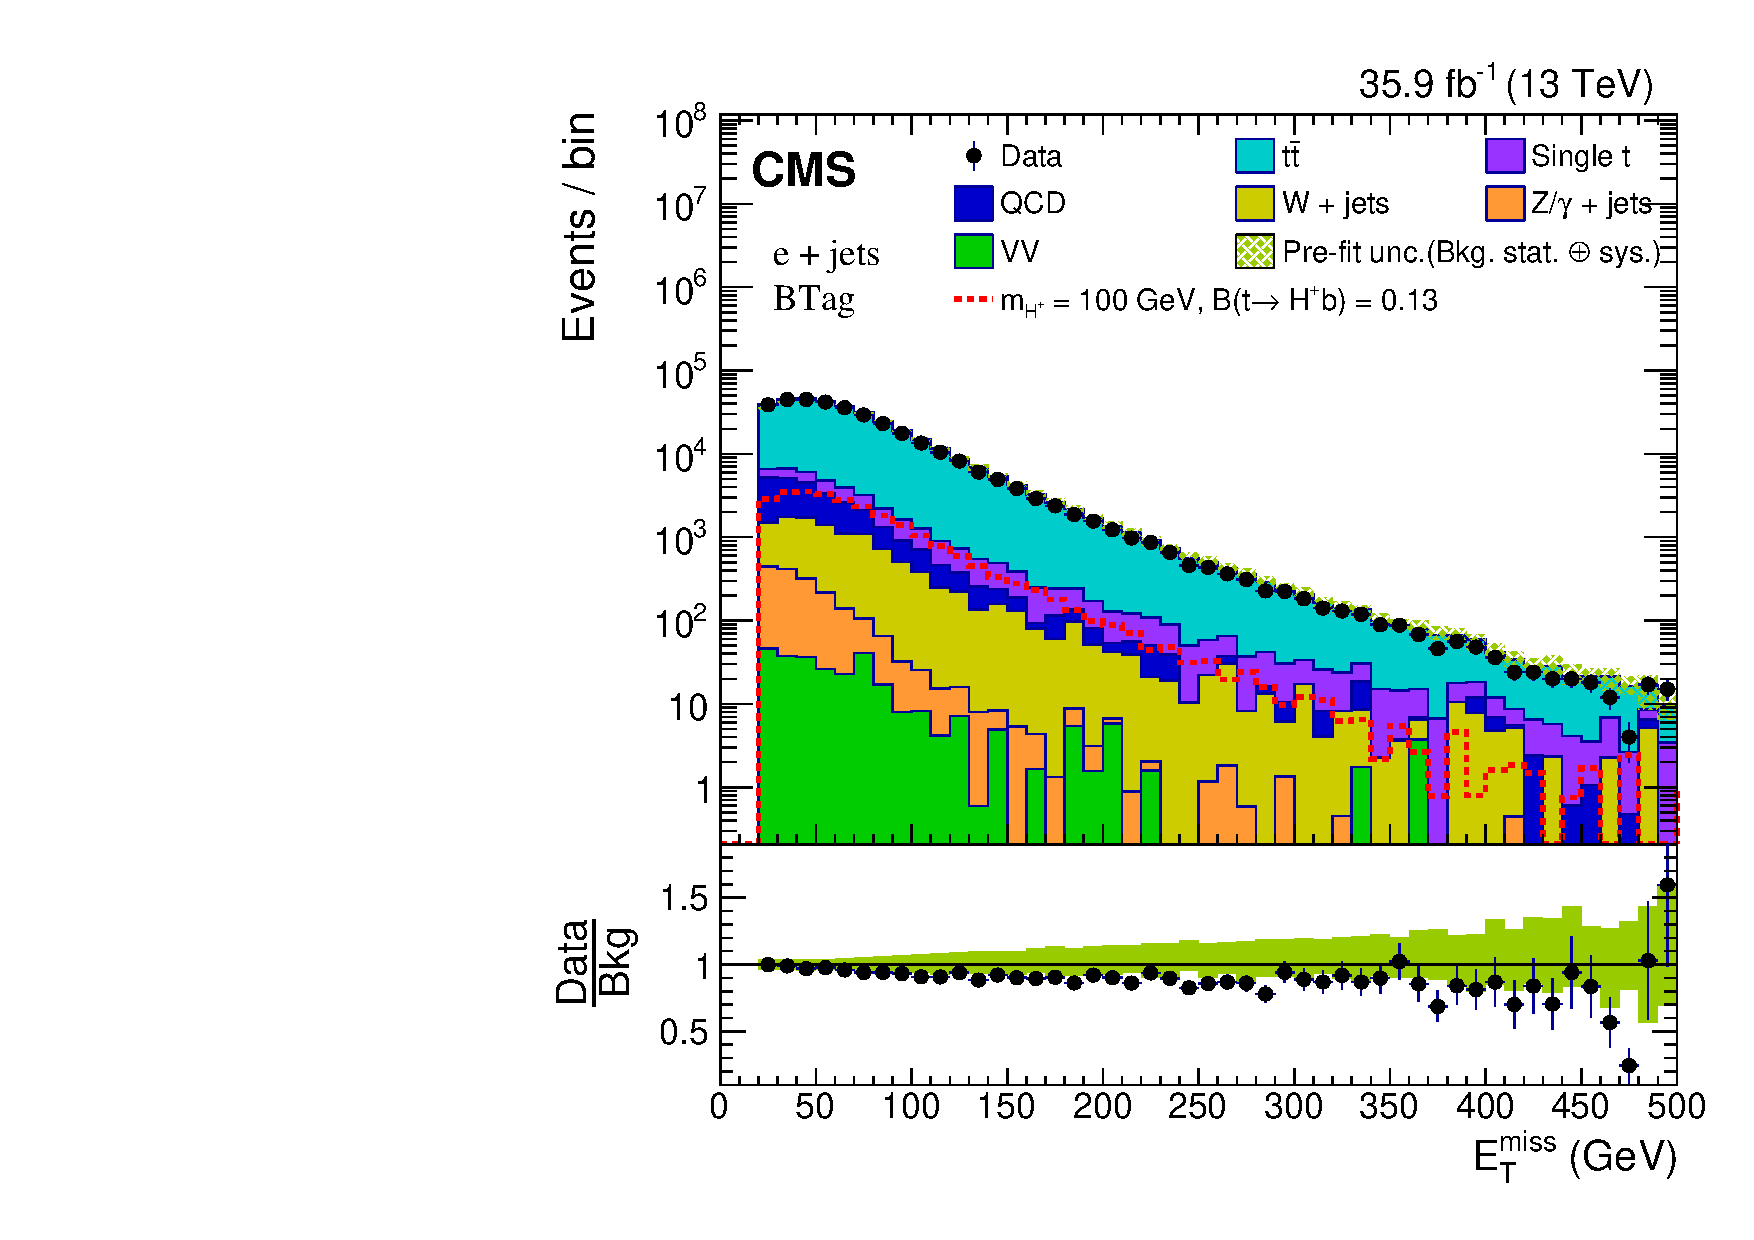
\includegraphics[width=0.45\linewidth]{Image/Electron/BTag/final_pt_met_eleBTag.pdf}}
    \vfil
    \subfigure[Transverse mass of W-boson]{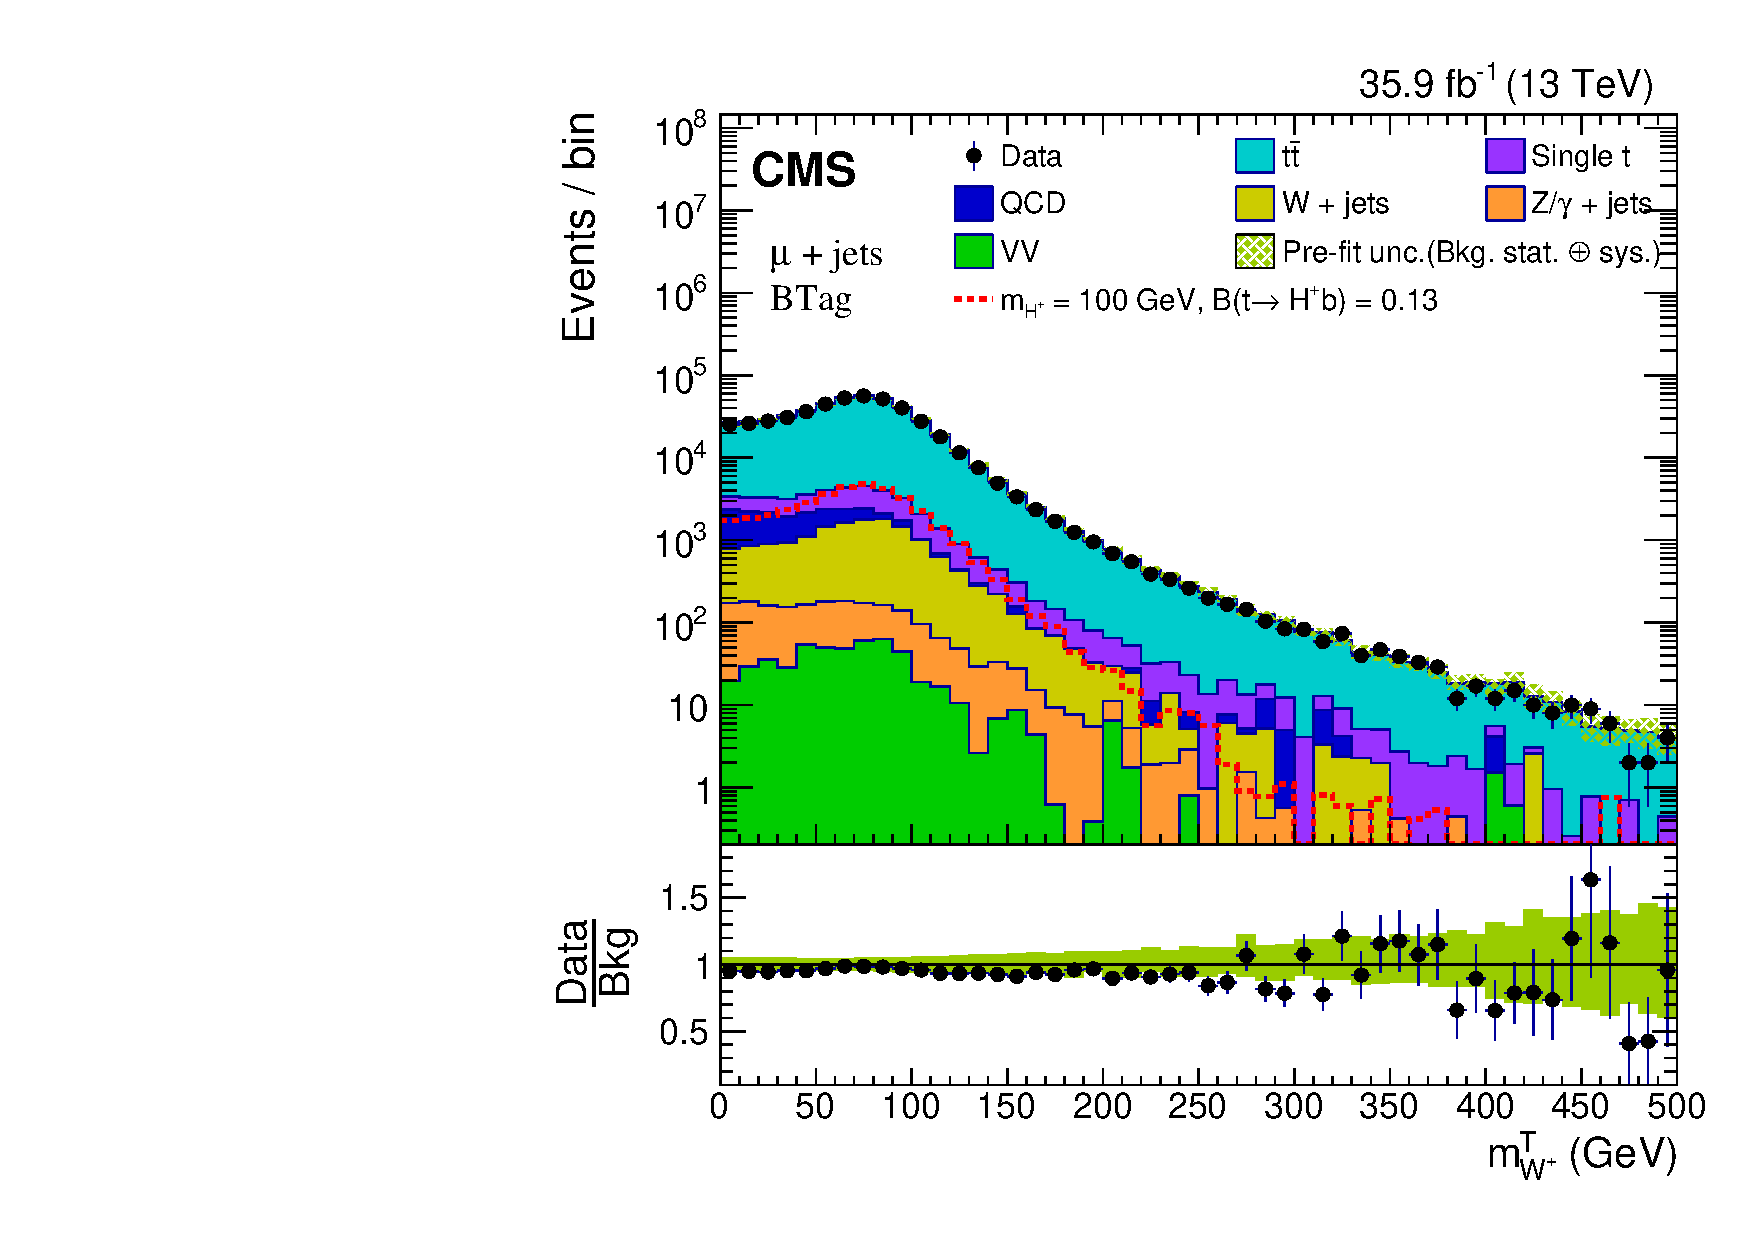
\includegraphics[width=0.45\linewidth]{Image/Muon/BTag/wmt_muBTag.pdf}}
    \subfigure[Transverse mass of W-boson]{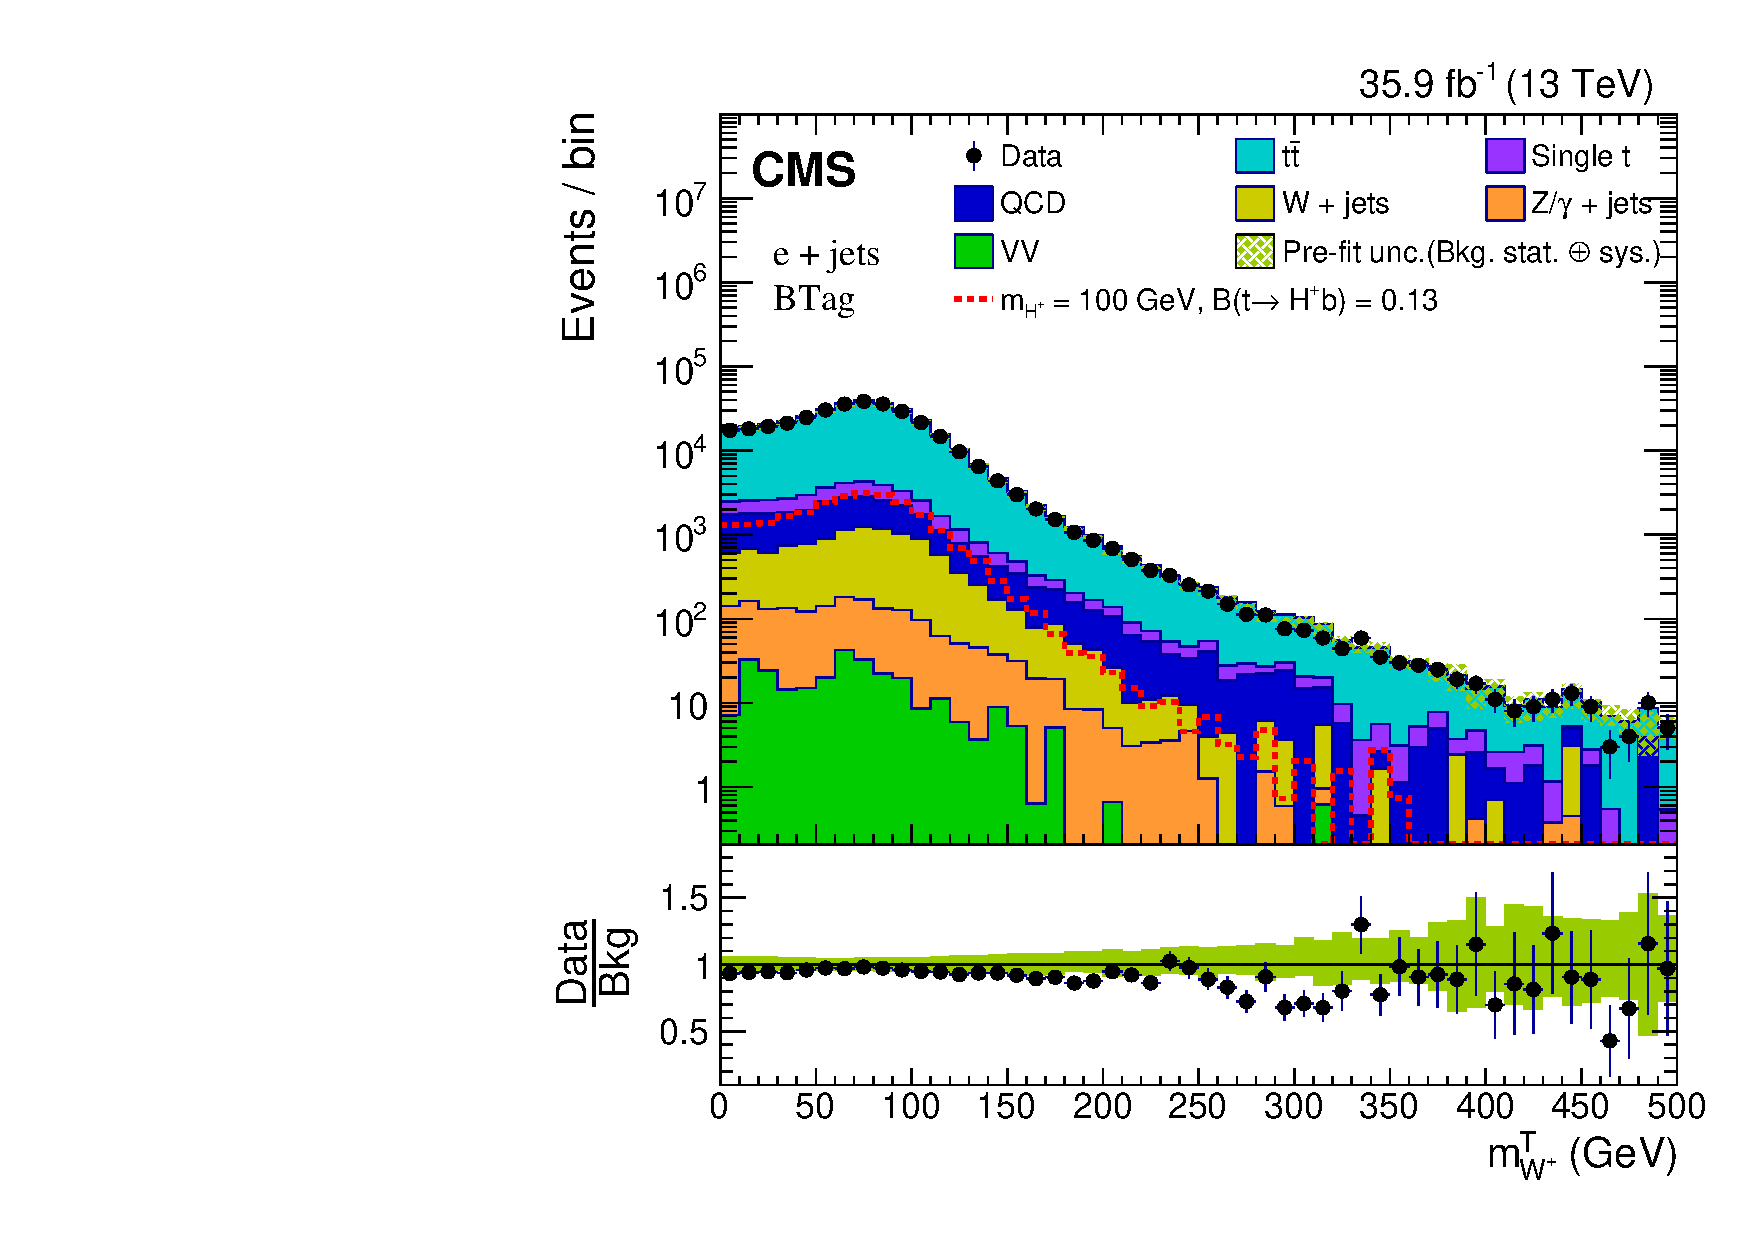
\includegraphics[width=0.45\linewidth]{Image/Electron/BTag/wmt_eleBTag.pdf}}
    \caption{Distribution of reconstructed $\MET$ and $m_{W^+}^{T}$ 
        (transverse mass of W-boson, W decaying leptonically) after b-jet 
        selection as described in Sec.~\ref{s:secEvtSel}, for muons + jets and 
    \ejets channel.}
    \label{fig:btagPlot3}
\end{figure}


%After KinFit: Pt_lep, Eta_lep, Pt_jets
\begin{figure}
    \centering  
    \subfigure[\pt of muons]{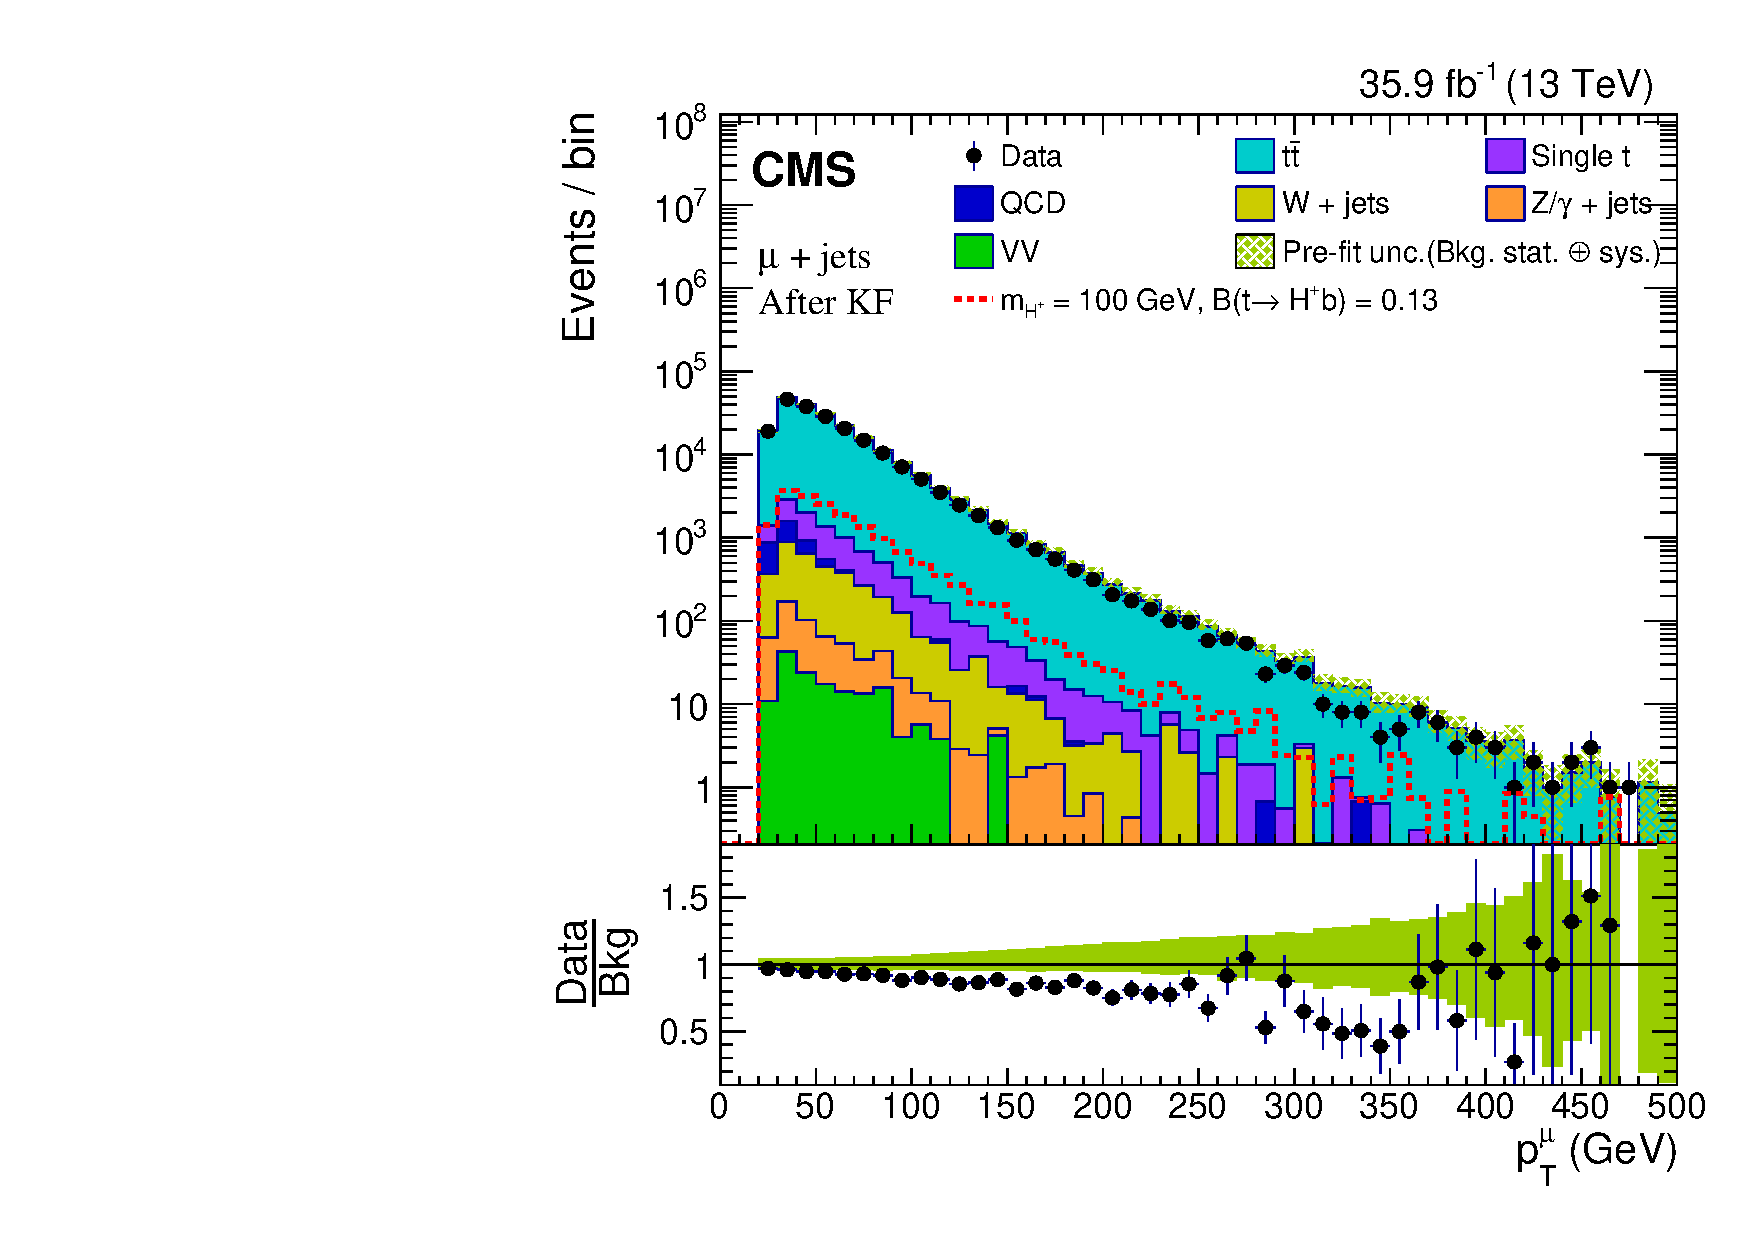
\includegraphics[width=0.45\linewidth]{Image/Muon/KinFit/pt_mu_muKinFit.pdf}}
    \subfigure[\pt of electrons]{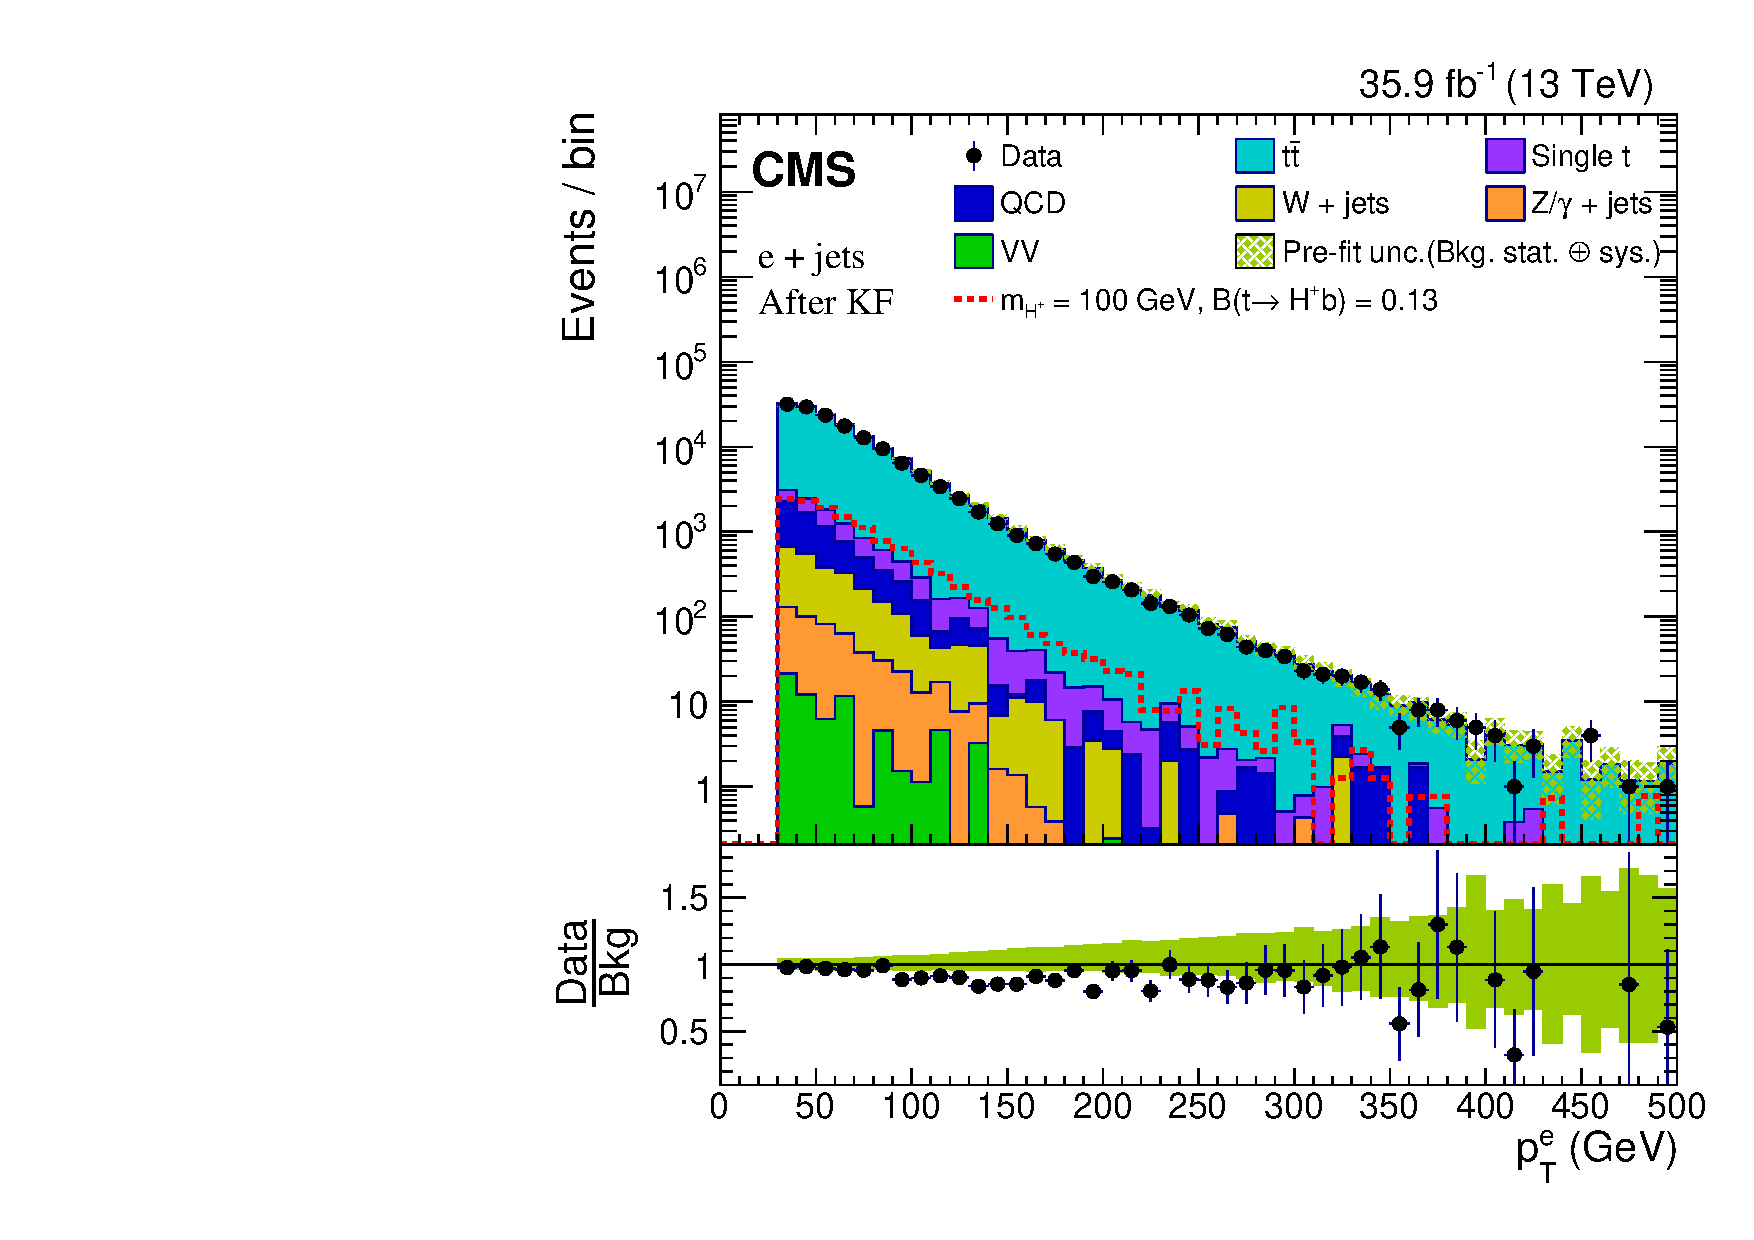
\includegraphics[width=0.45\linewidth]{Image/Electron/KinFit/pt_ele_eleKinFit.pdf}}
    \vfil
    \subfigure[$\eta$ of muons]{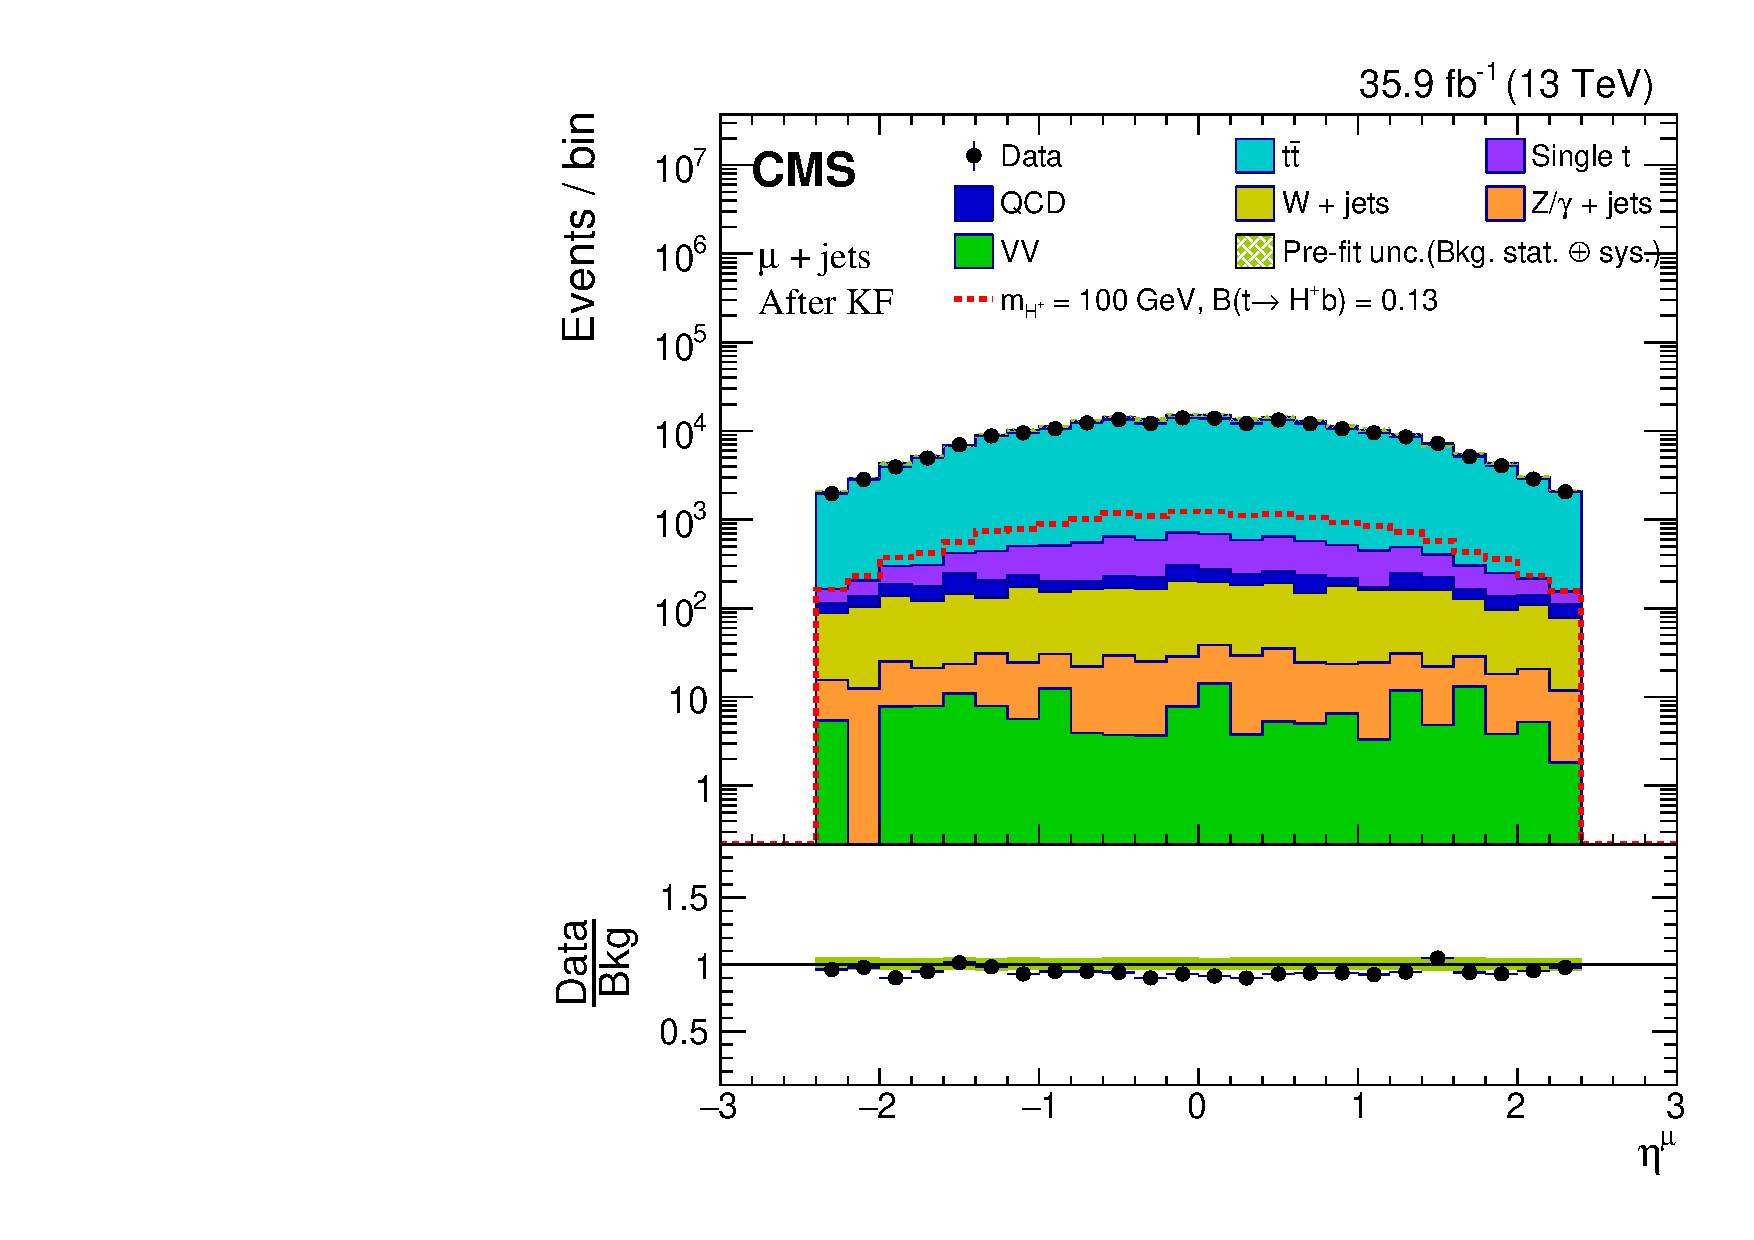
\includegraphics[width=0.45\linewidth]{Image/Muon/KinFit/eta_mu_muKinFit.pdf}}
    \subfigure[$\eta$ of electrons]{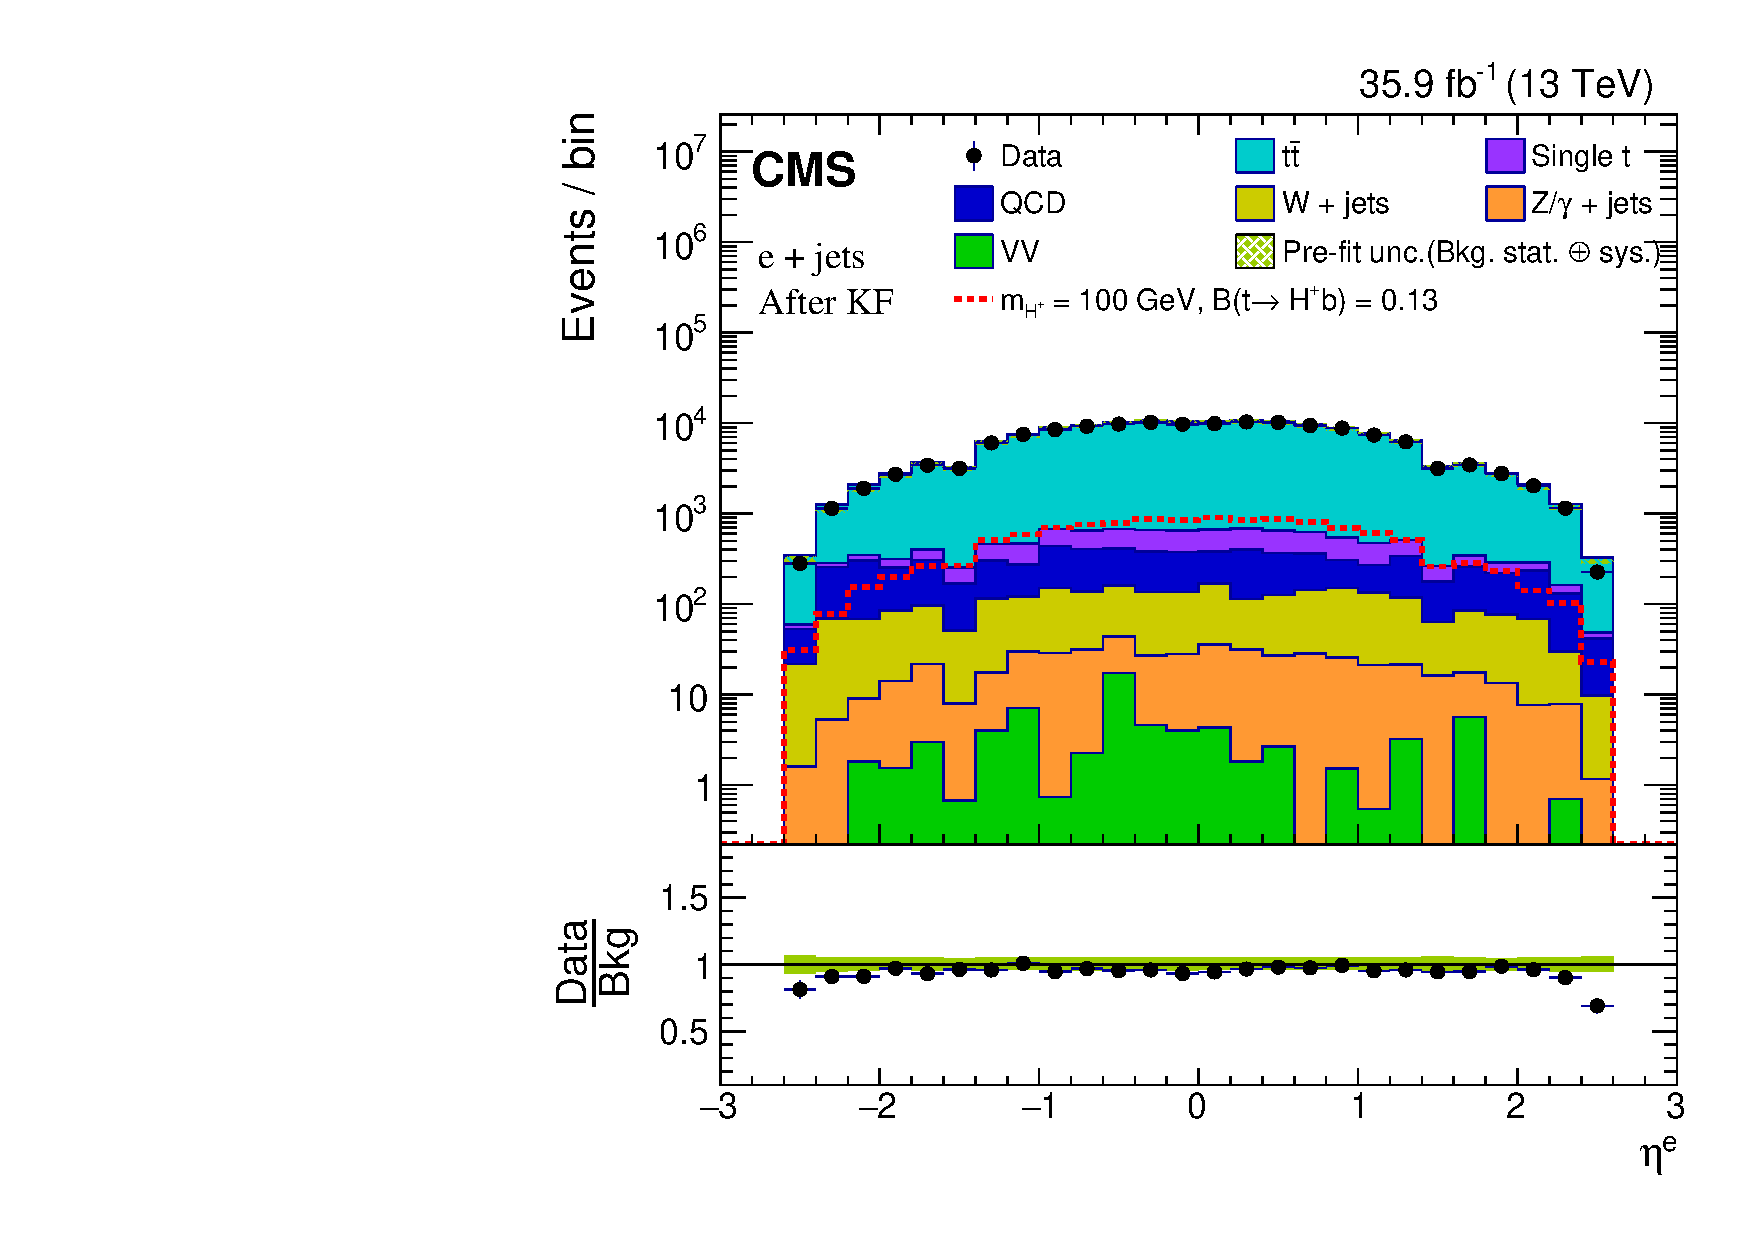
\includegraphics[width=0.45\linewidth]{Image/Electron/KinFit/eta_ele_eleKinFit.pdf}}
    \vfil
    \subfigure[\pt of jets]{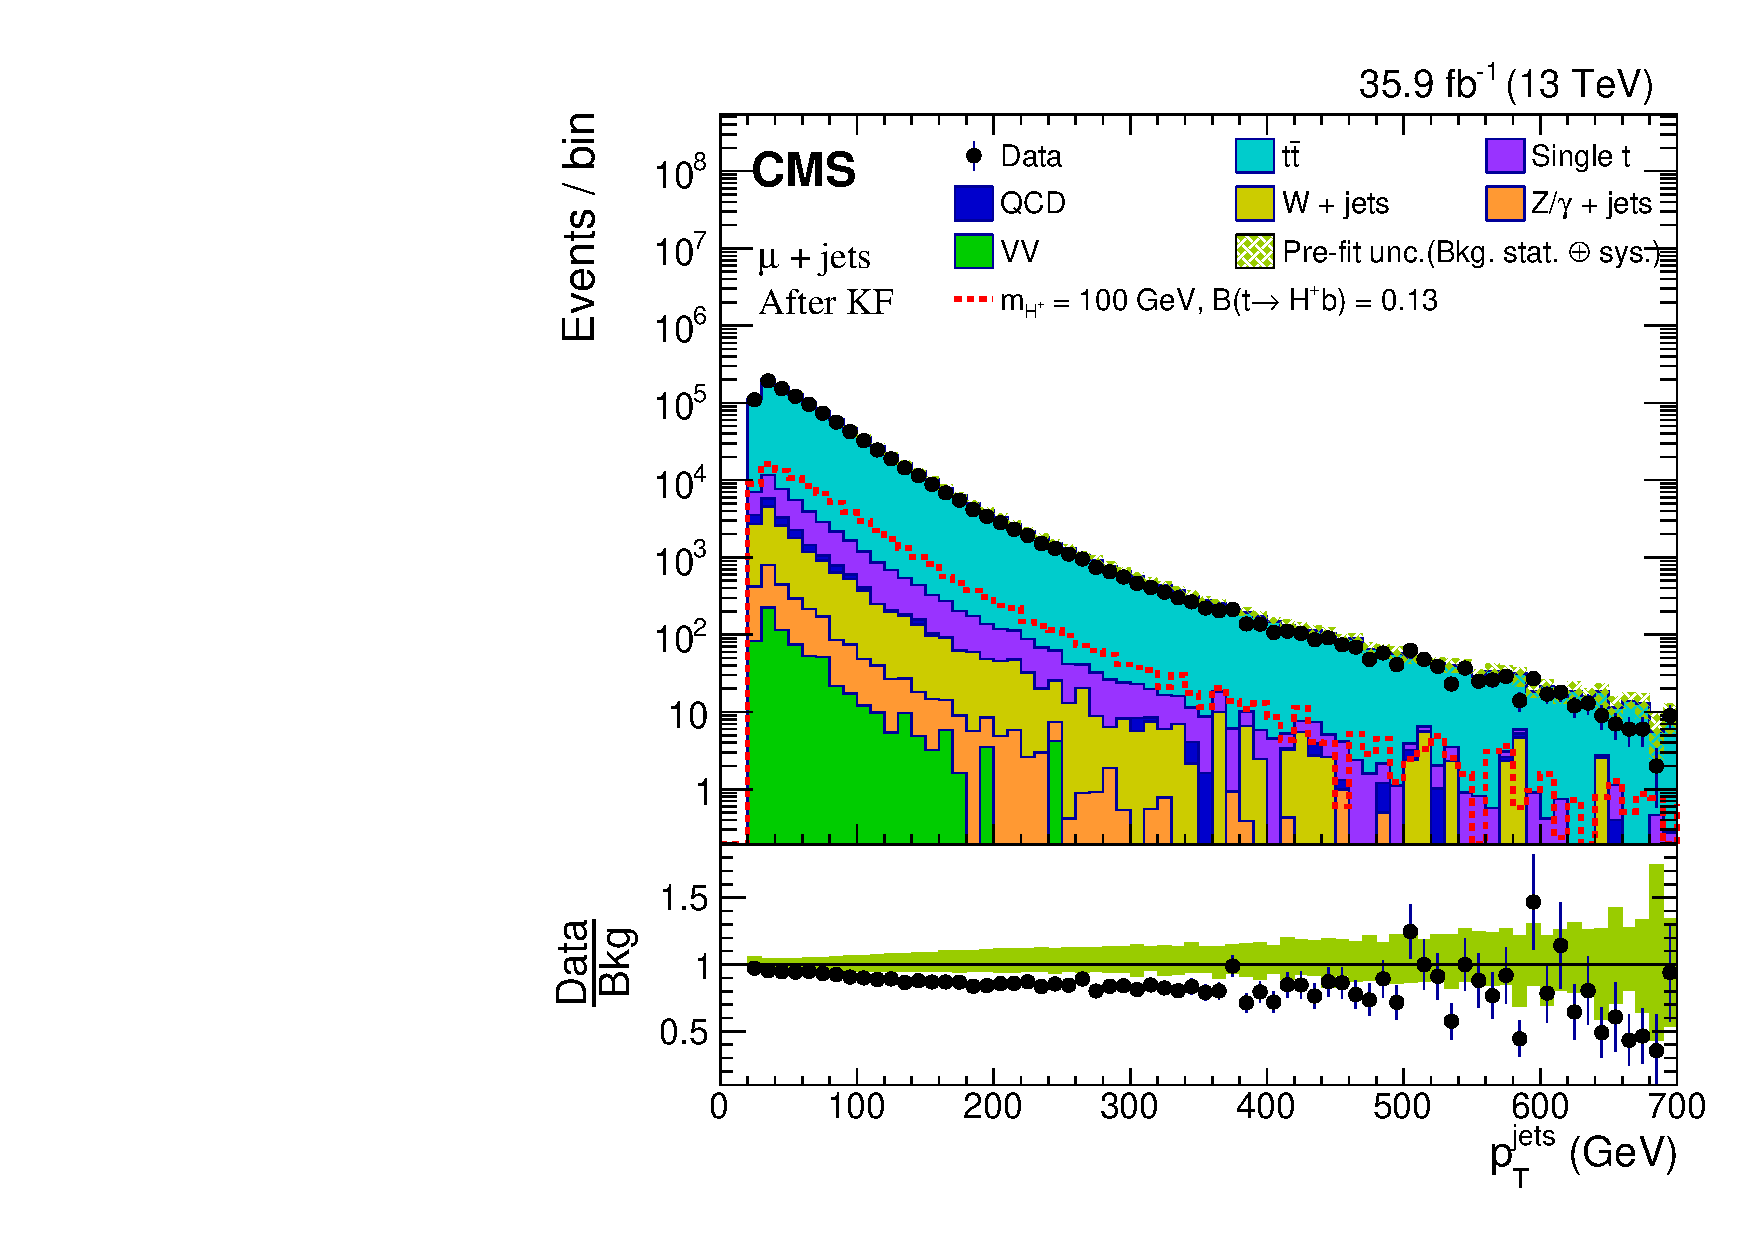
\includegraphics[width=0.45\linewidth]{Image/Muon/KinFit/pt_jet_muKinFit.pdf}}
    \subfigure[\pt of jets]{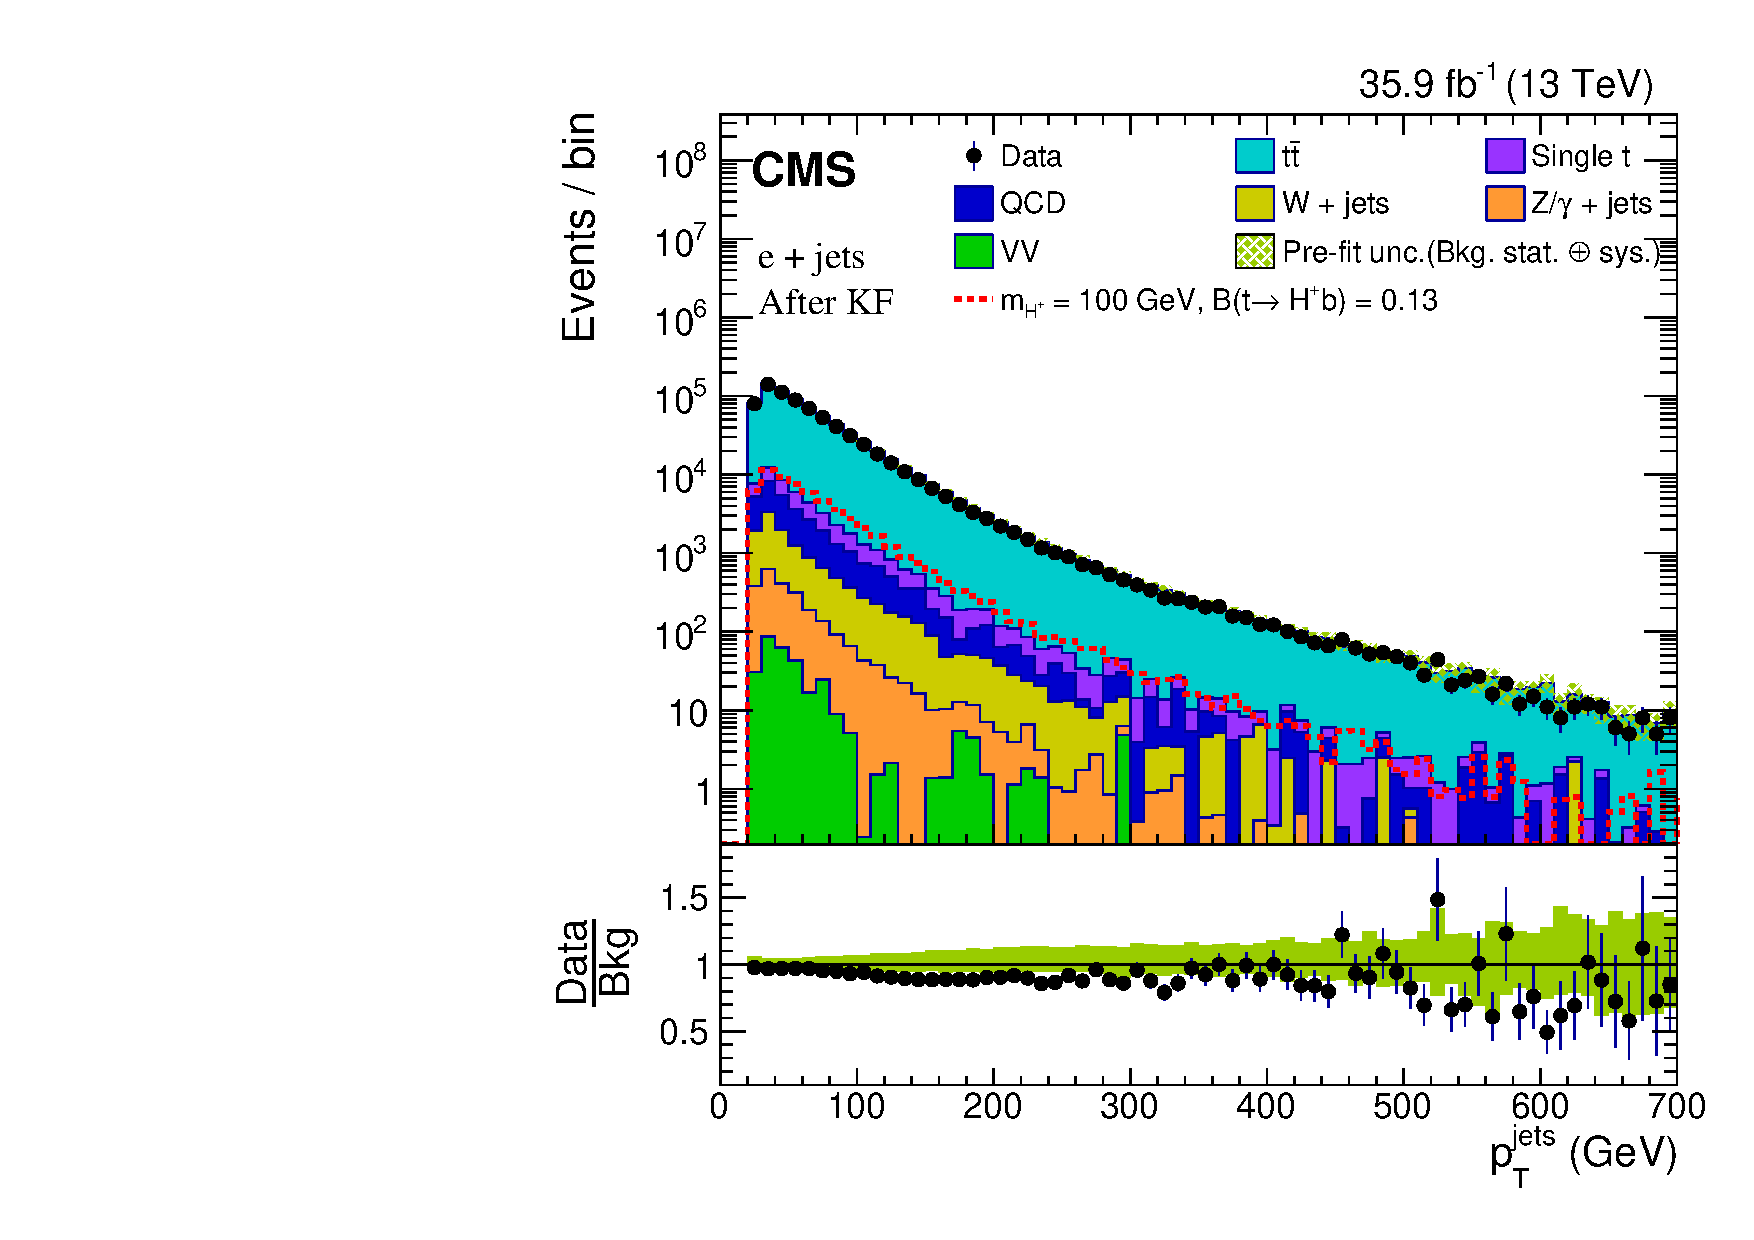
\includegraphics[width=0.45\linewidth]{Image/Electron/KinFit/pt_jet_eleKinFit.pdf}}
    \caption{Distribution of $\pt, \eta$ of kinematic fitted lepton and $\pt$ of jets
    after kinematic fit selection as described in Sec.~\ref{s:secEvtSel}, 
for muons + jets and \ejets channel.}
    \label{fig:kfitPlot1}
\end{figure}

%After KinFit:Eta_jets , N_jets, N_bjets
\begin{figure}
    \centering  
    \subfigure[$\eta$ of jets]{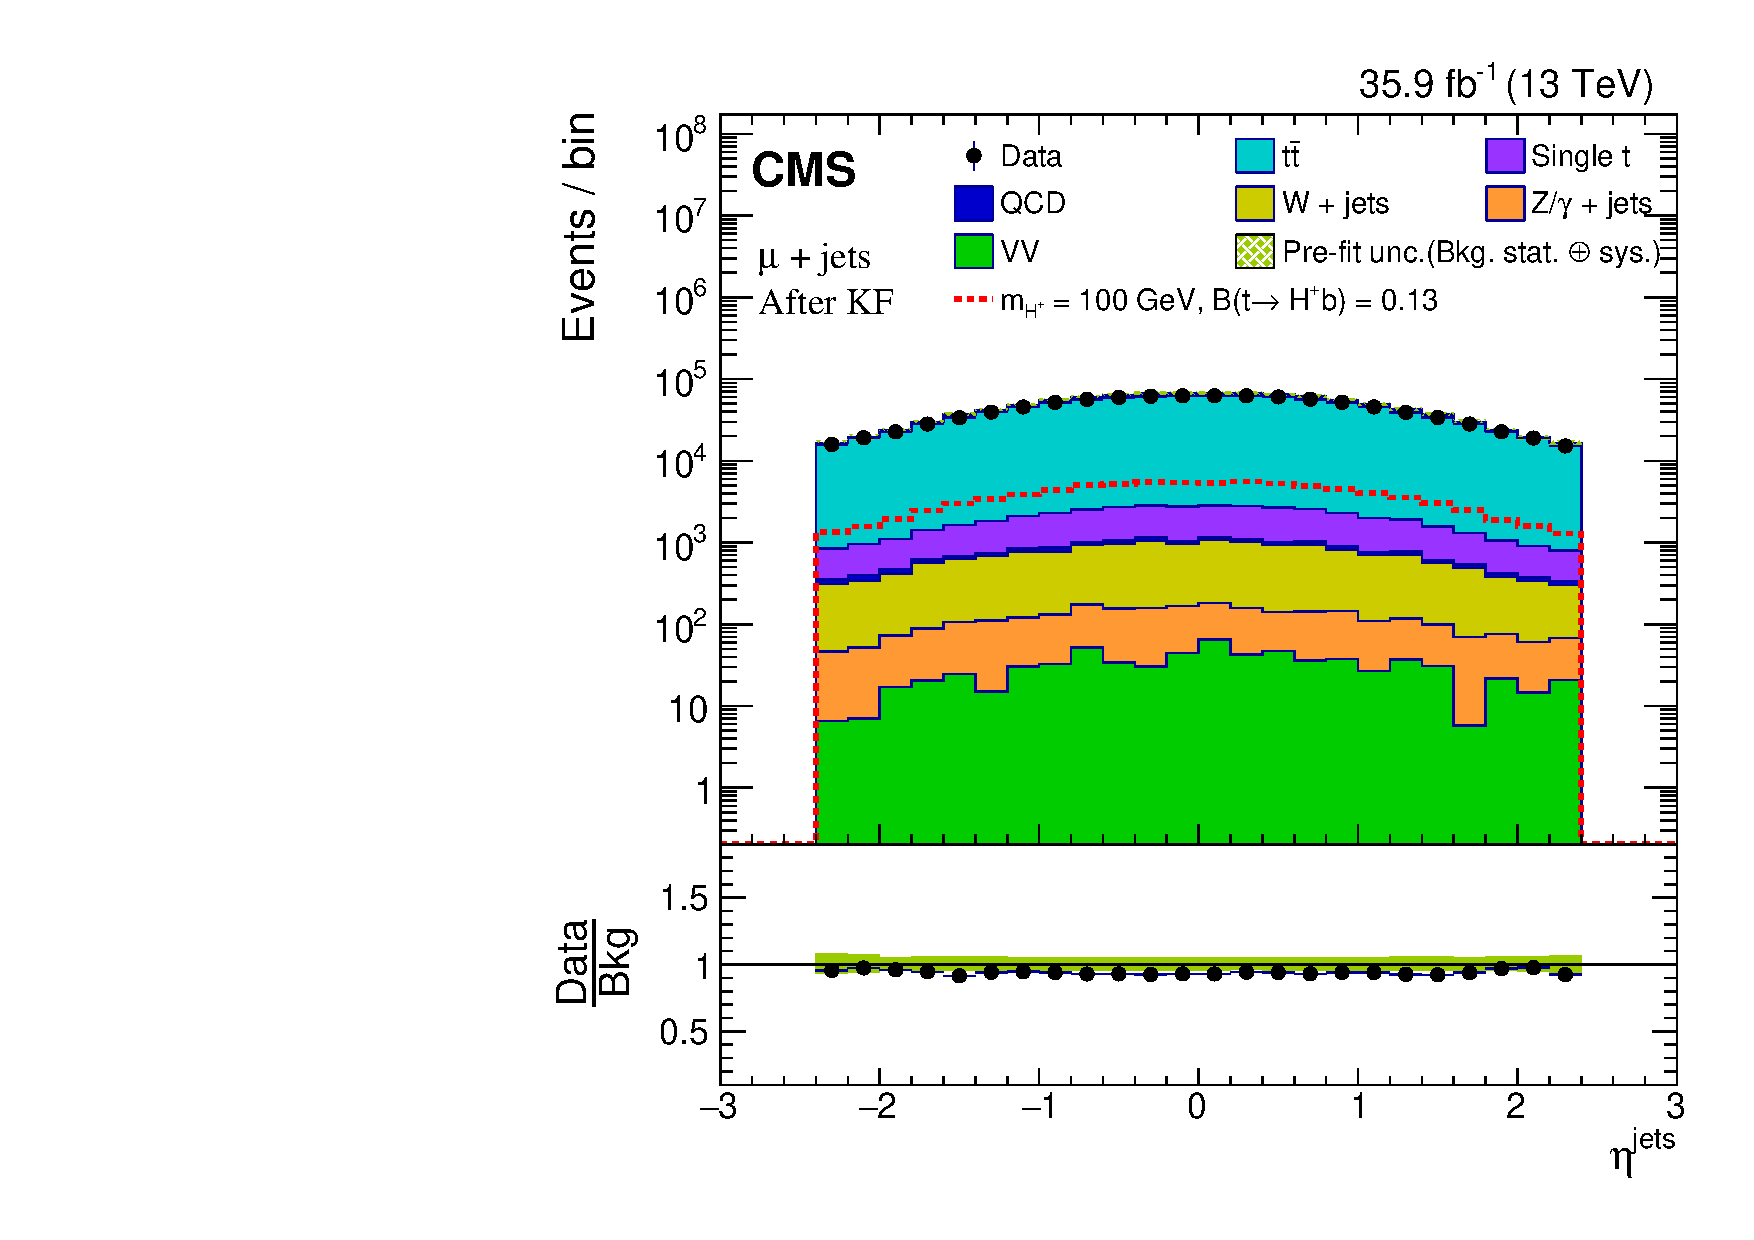
\includegraphics[width=0.45\linewidth]{Image/Muon/KinFit/eta_jet_muKinFit.pdf}}
    \subfigure[$\eta$ of jets]{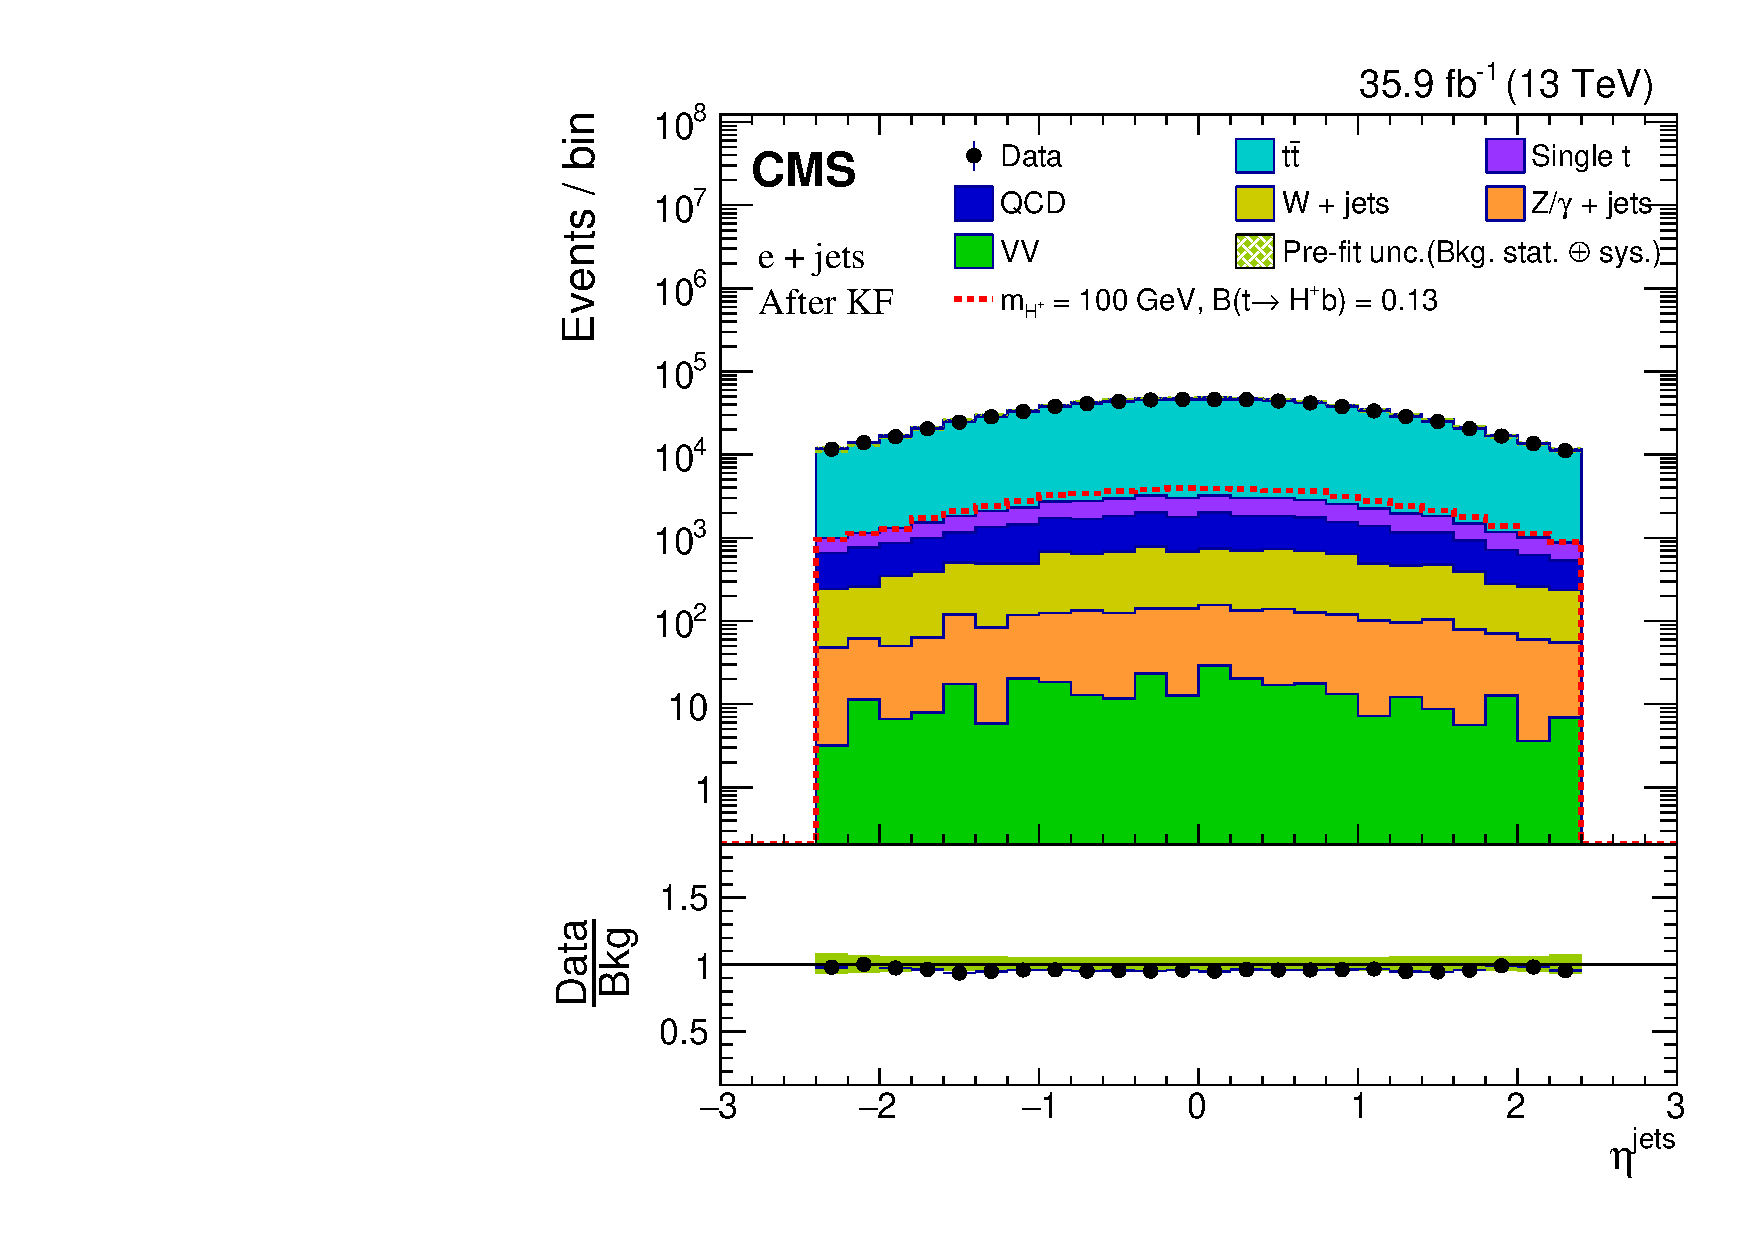
\includegraphics[width=0.45\linewidth]{Image/Electron/KinFit/eta_jet_eleKinFit.pdf}}
    \vfil
    \subfigure[jet multiplicity]{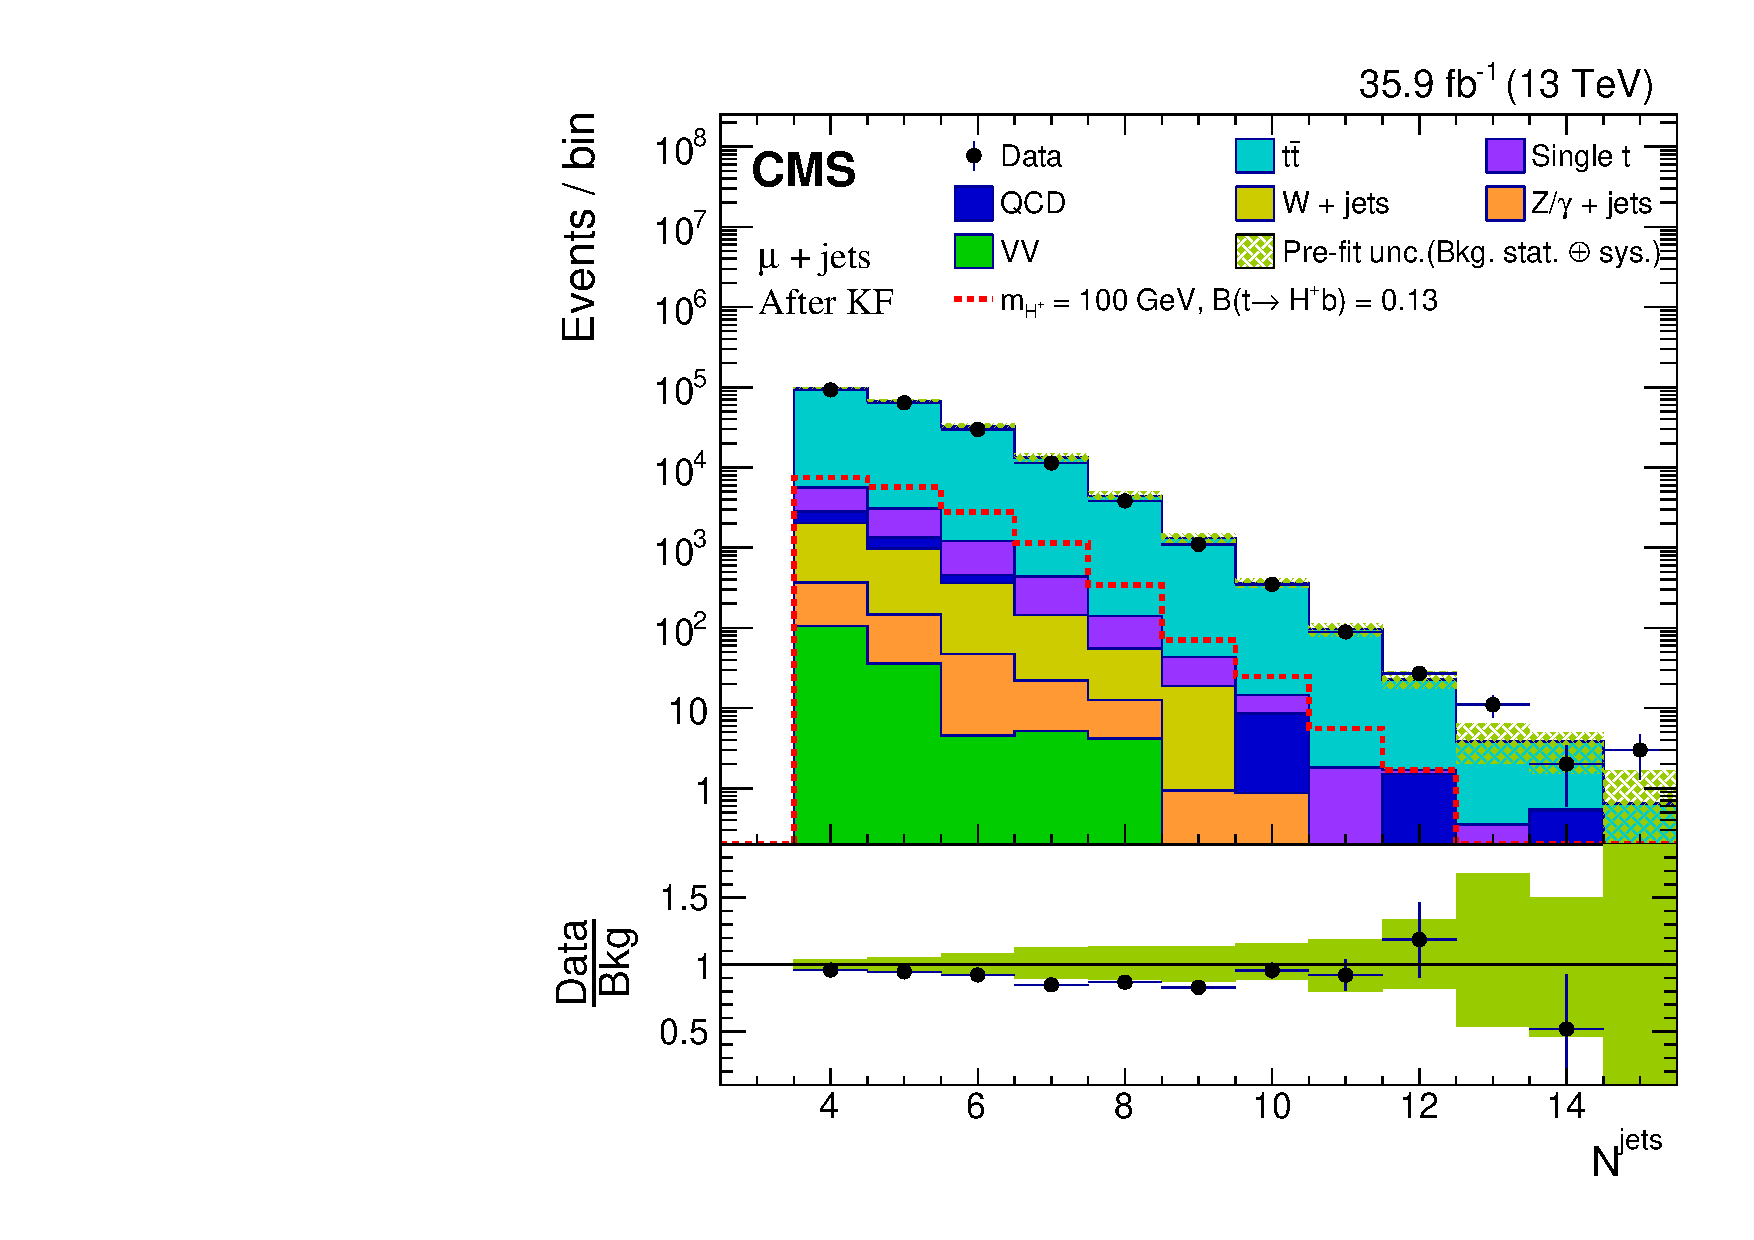
\includegraphics[width=0.45\linewidth]{Image/Muon/KinFit/final_multi_jet_muKinFit.pdf}}
    \subfigure[jet multiplicity]{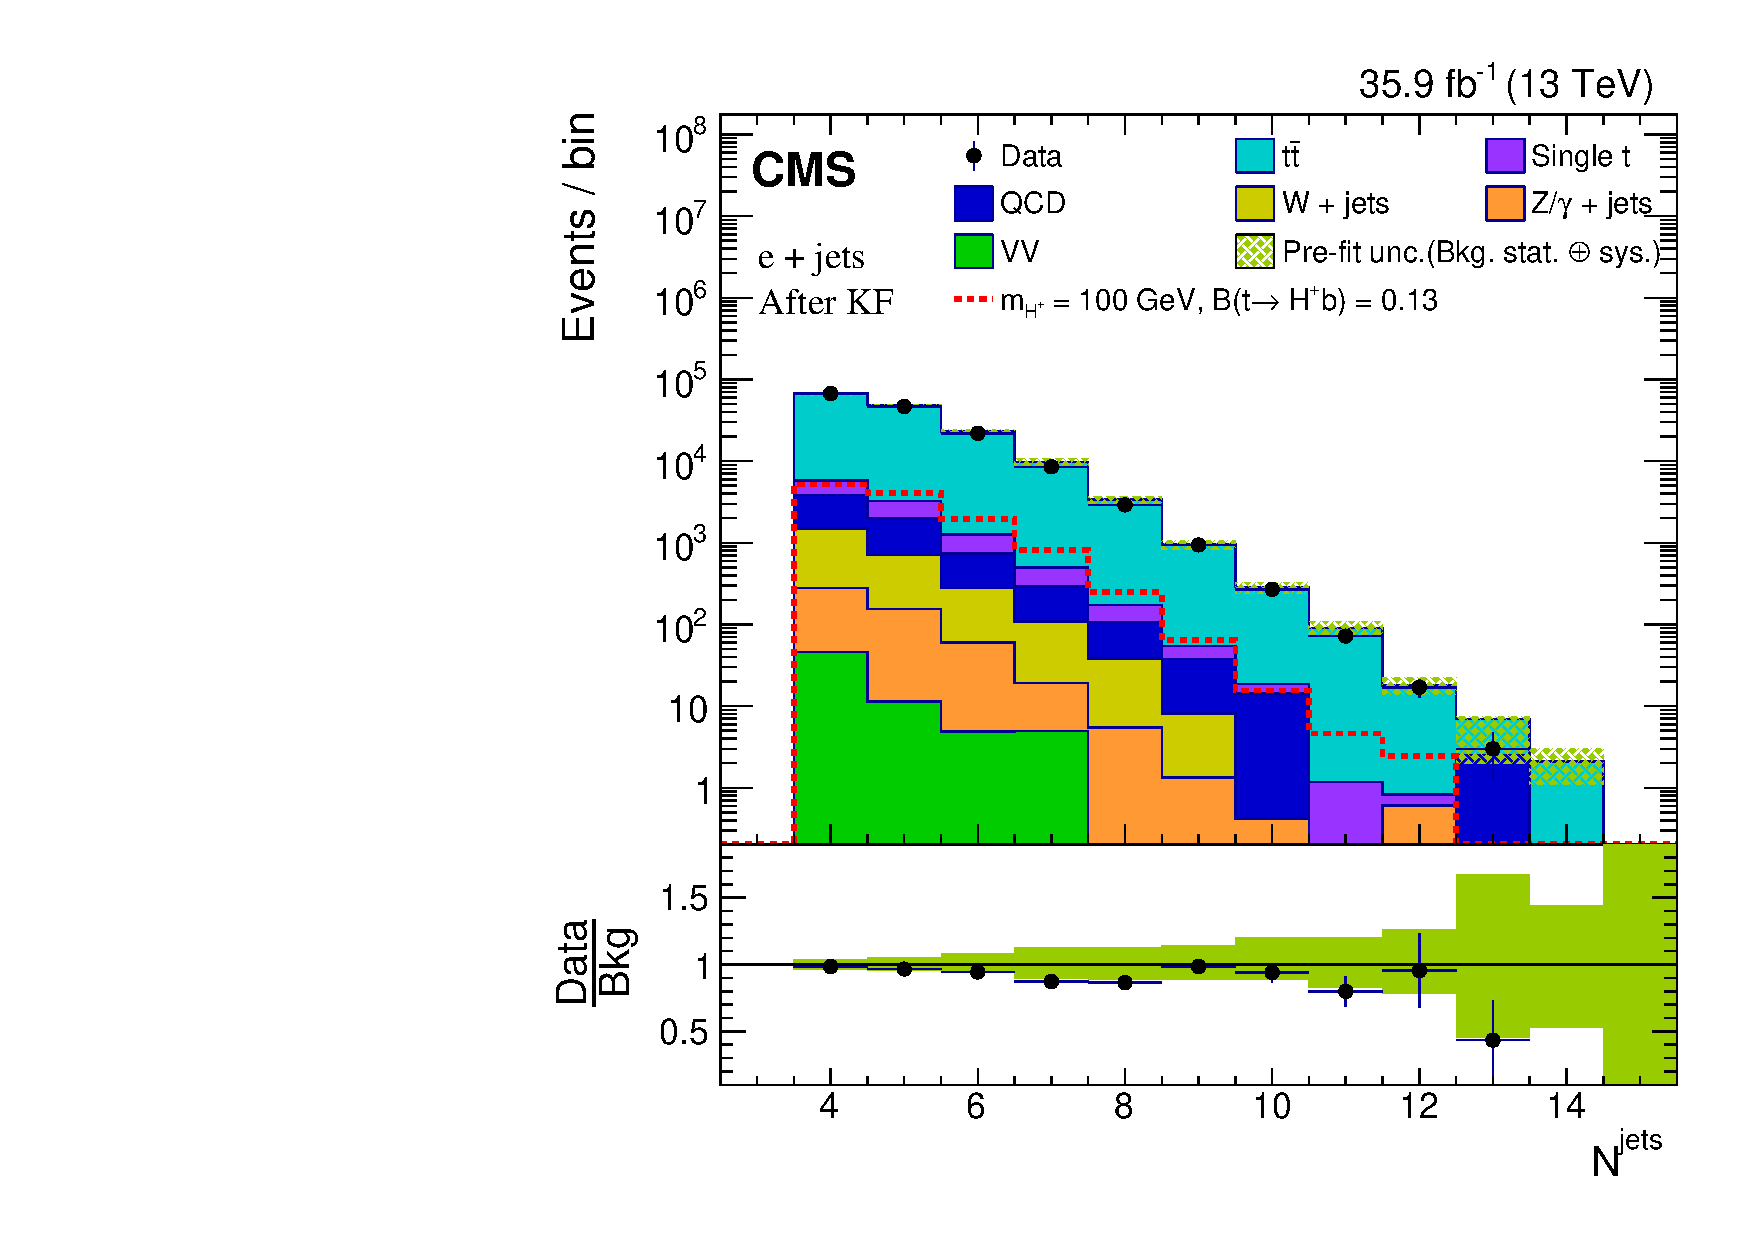
\includegraphics[width=0.45\linewidth]{Image/Electron/KinFit/final_multi_jet_eleKinFit.pdf}}
    \vfil
    \subfigure[b-jet multiplicity]{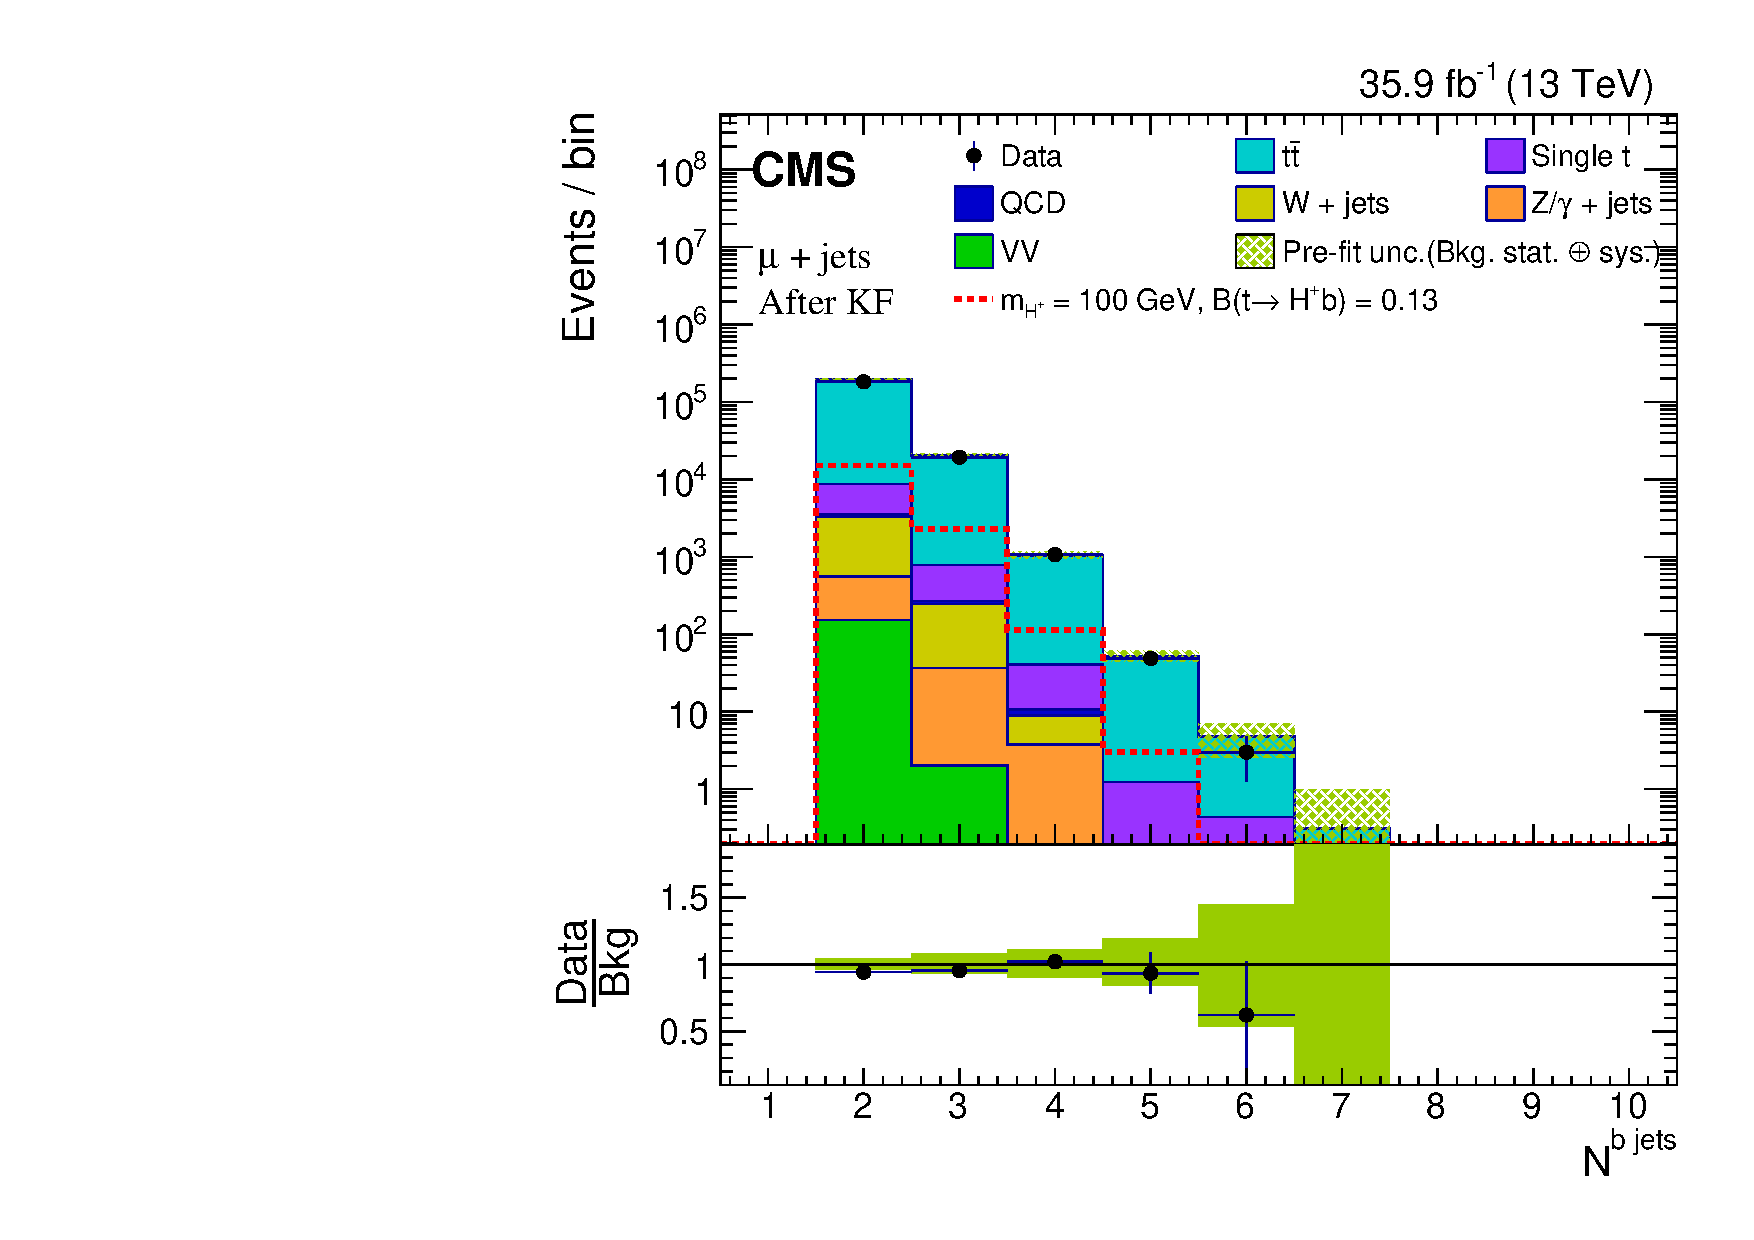
\includegraphics[width=0.45\linewidth]{Image/Muon/KinFit/CSVL_count_muKinFit.pdf}}
    \subfigure[b-jet multiplicity]{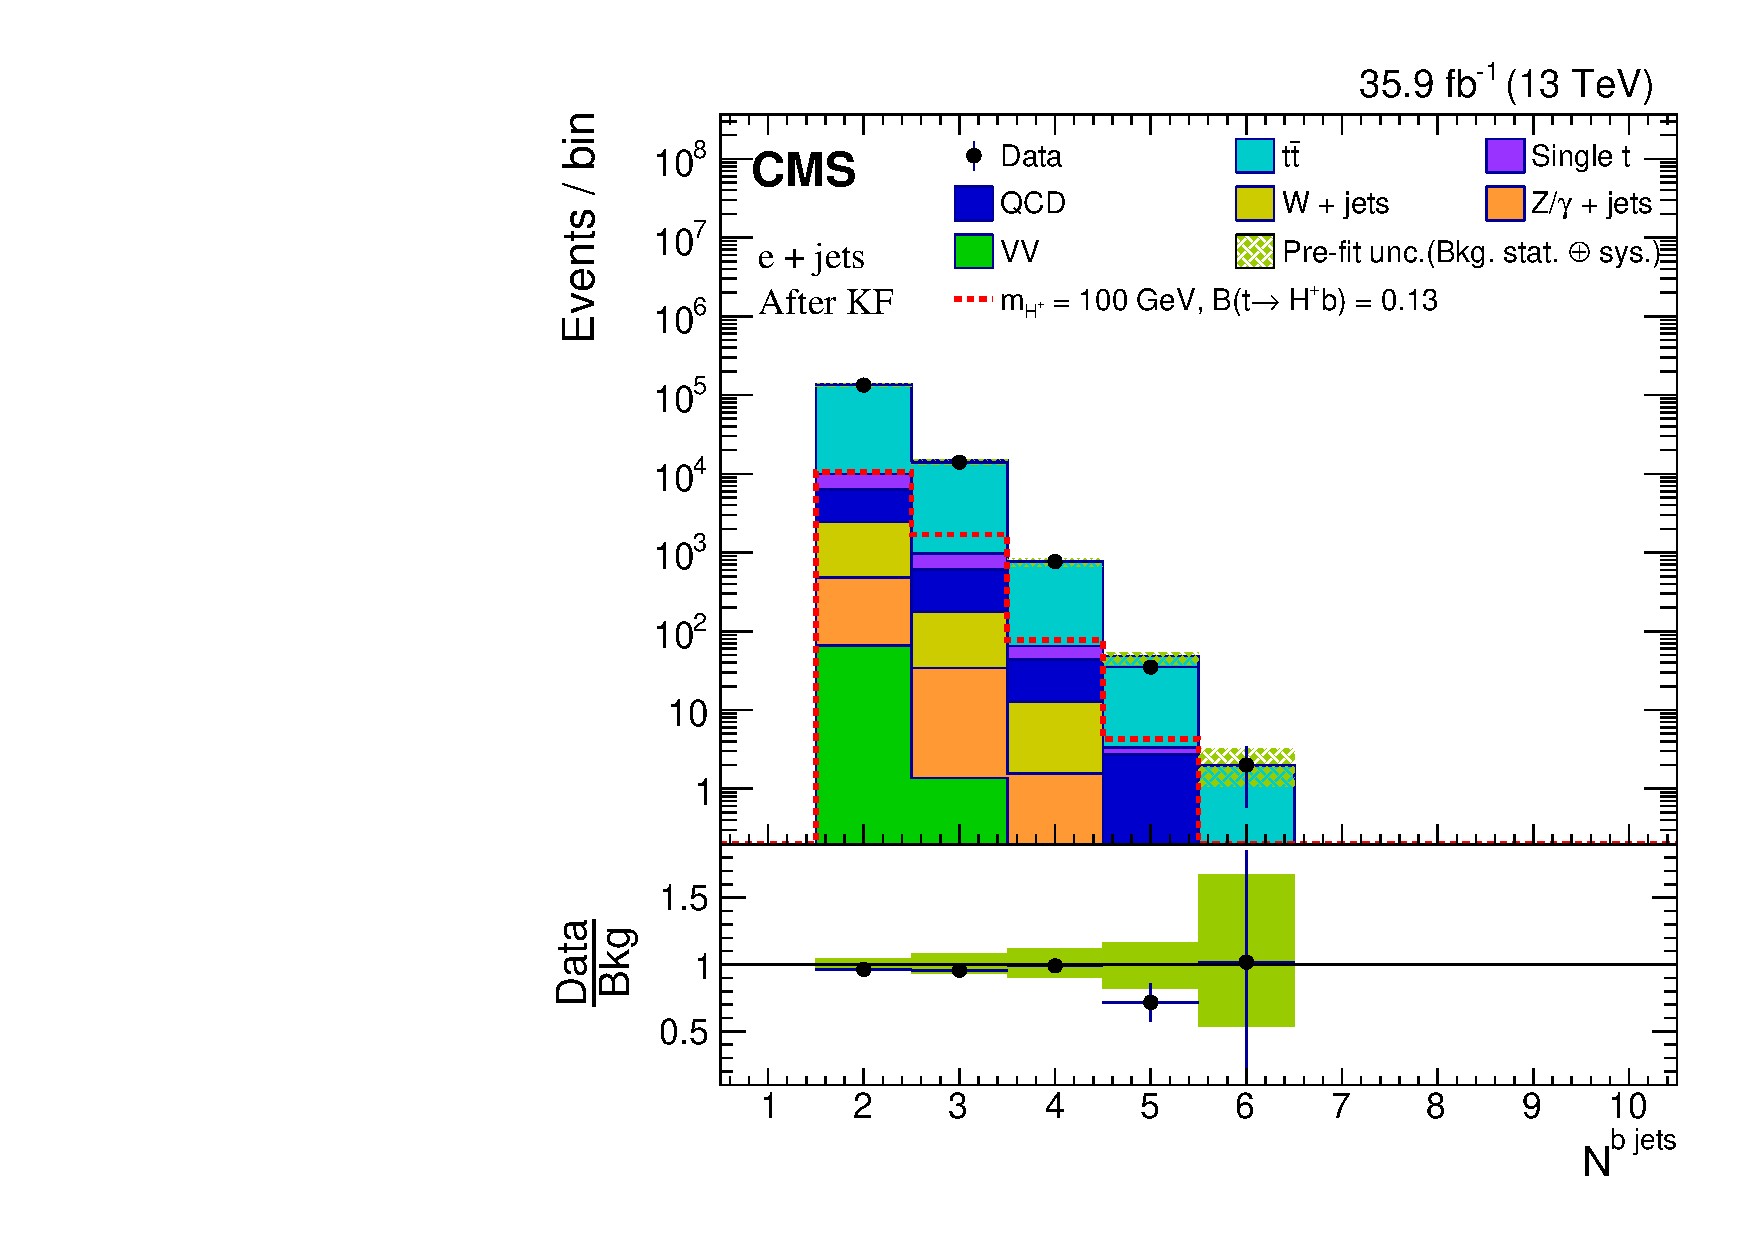
\includegraphics[width=0.45\linewidth]{Image/Electron/KinFit/CSVL_count_eleKinFit.pdf}}
    \caption{Distribution of kinematic fitted $\eta$ of jets, jet-multiplicity, and b-jet
        multiplicity after kinematic fit selection as described
        in Sec.~\ref{s:secEvtSel}, for muons + jets and \ejets
    channel.}
    \label{fig:kfitPlot2}
\end{figure}

\begin{figure}
    \centering  
    \subfigure[\MET]{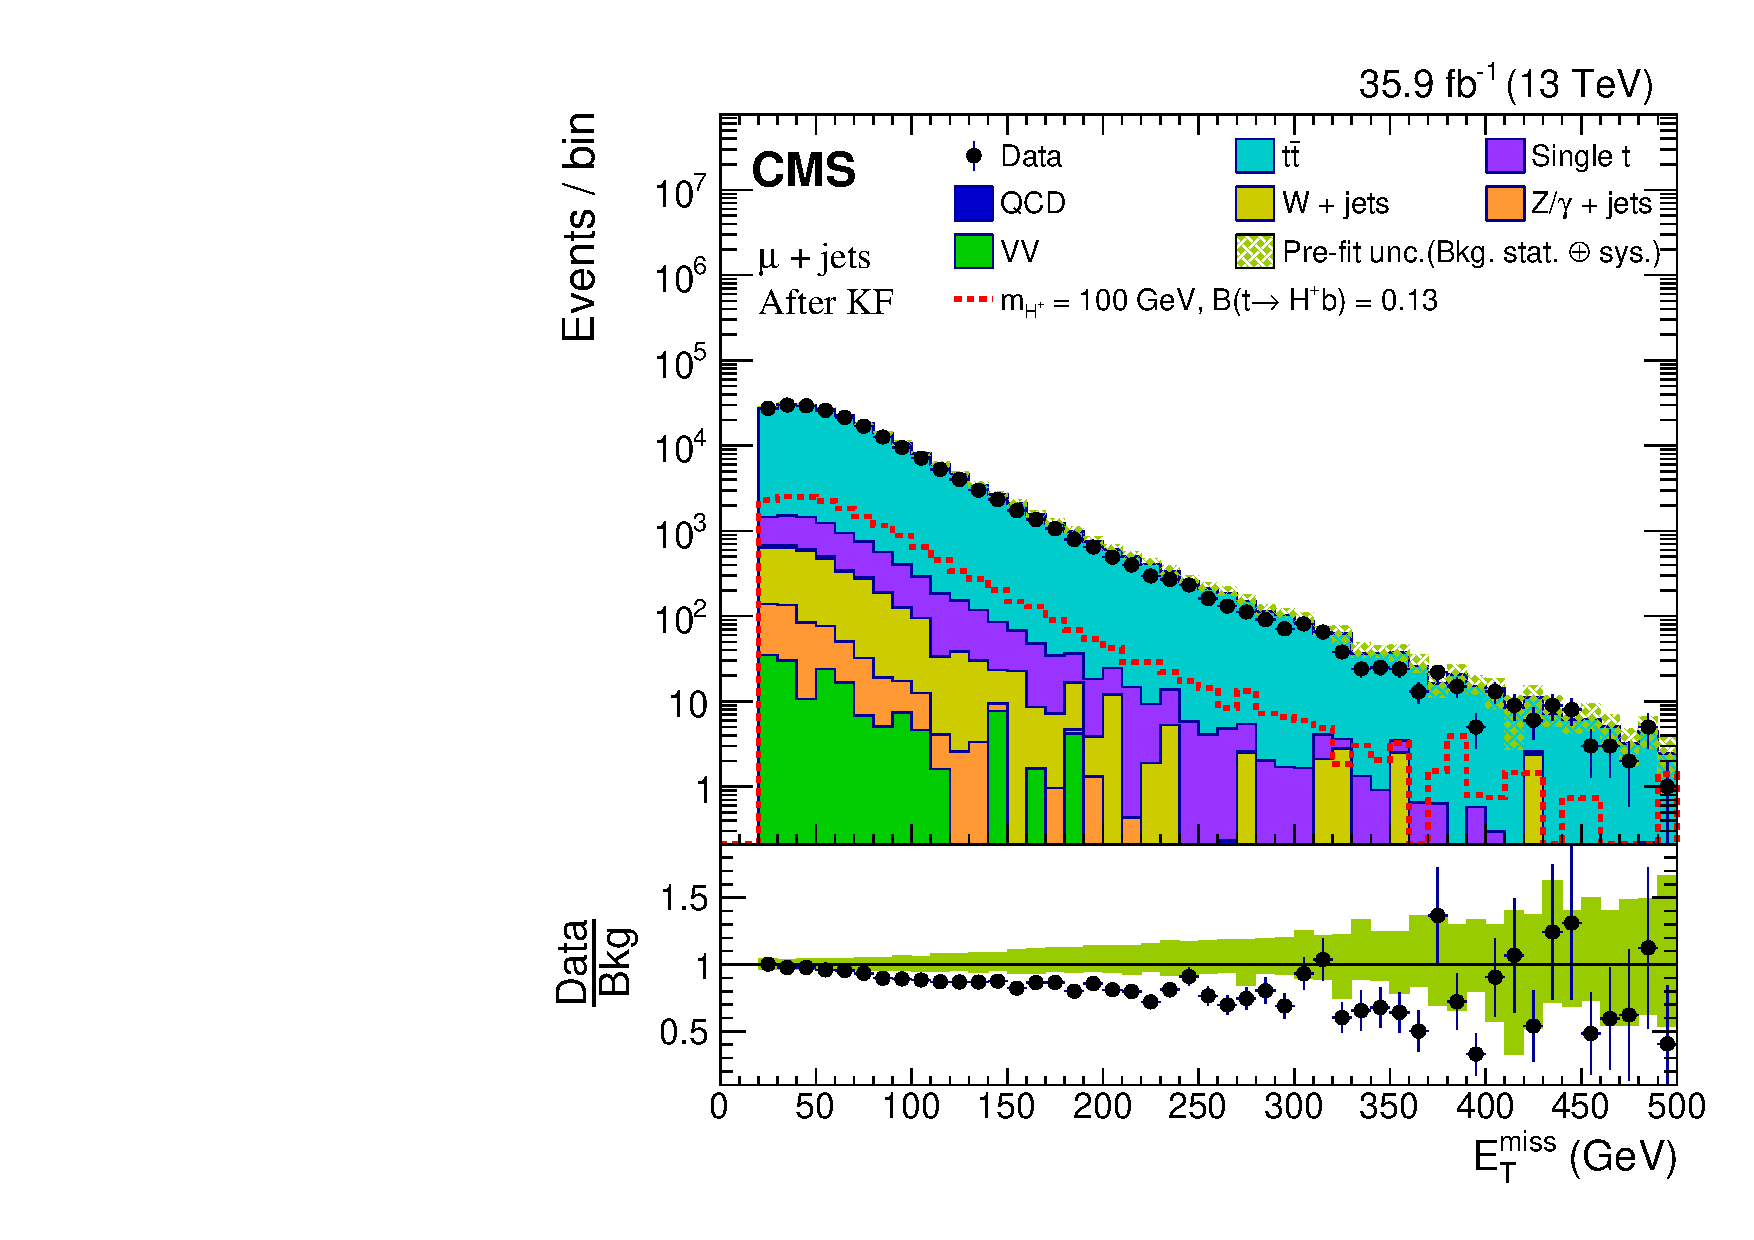
\includegraphics[width=0.45\linewidth]{Image/Muon/KinFit/final_pt_met_muKinFit.pdf}}
    \subfigure[\MET]{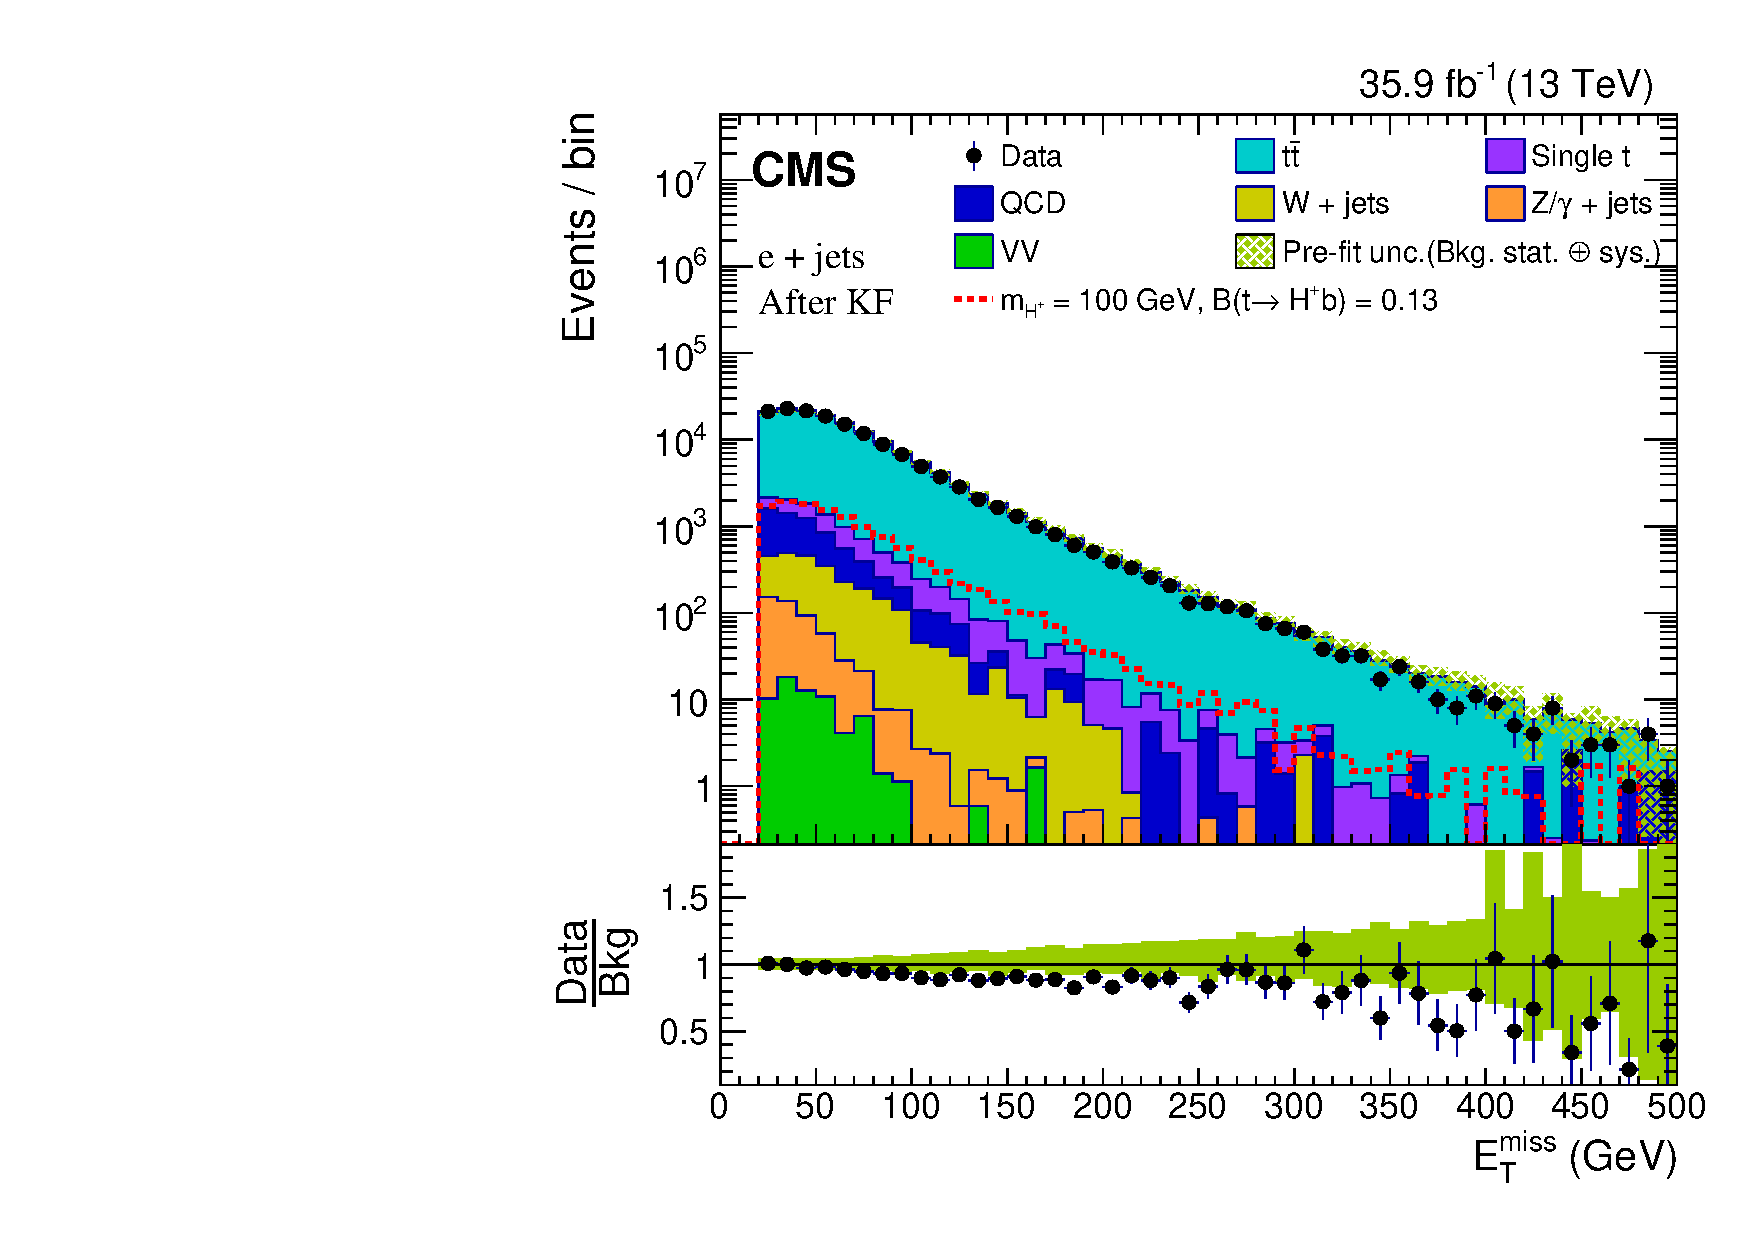
\includegraphics[width=0.45\linewidth]{Image/Electron/KinFit/final_pt_met_eleKinFit.pdf}}
    \vfil
    \subfigure[Transverse mass of W-boson]{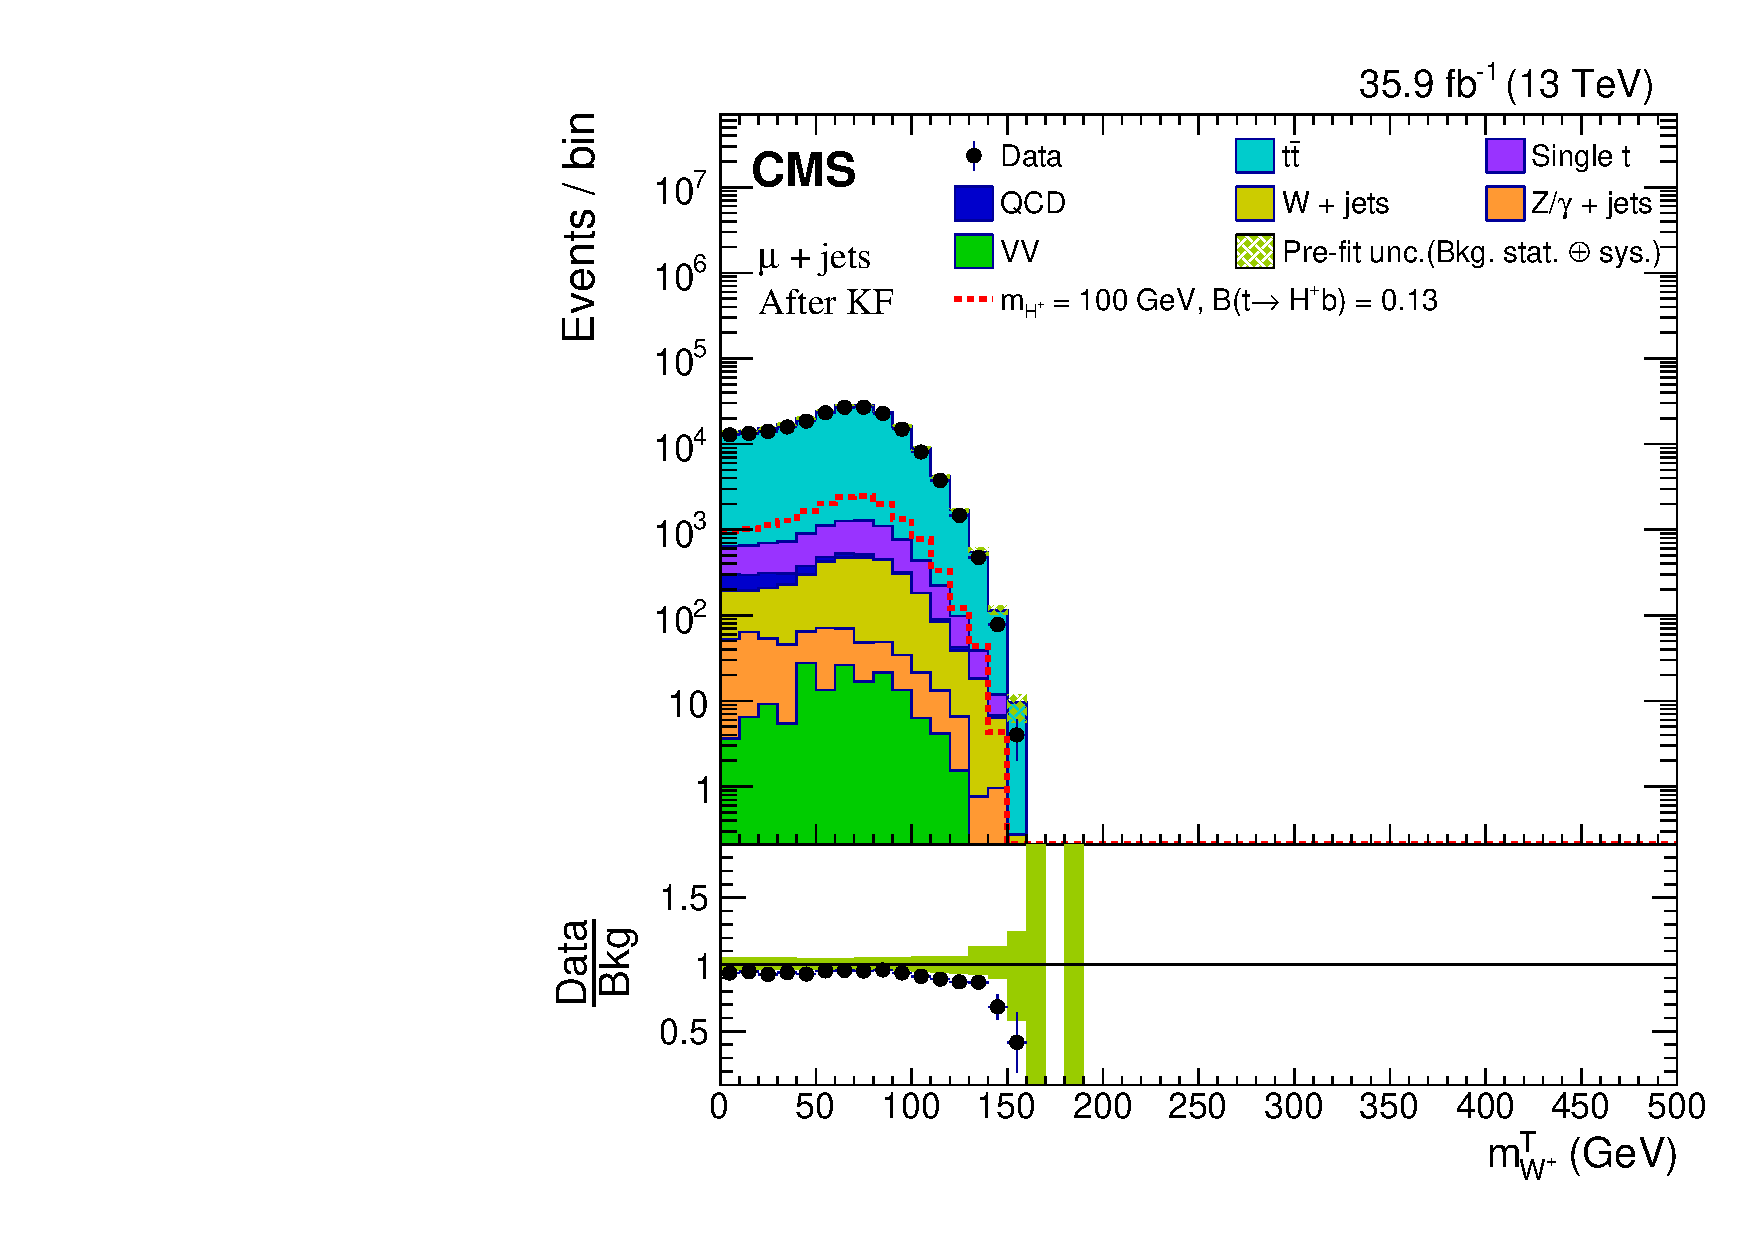
\includegraphics[width=0.45\linewidth]{Image/Muon/KinFit/wmt_muKinFit.pdf}}
    \subfigure[Transverse mass of W-boson]{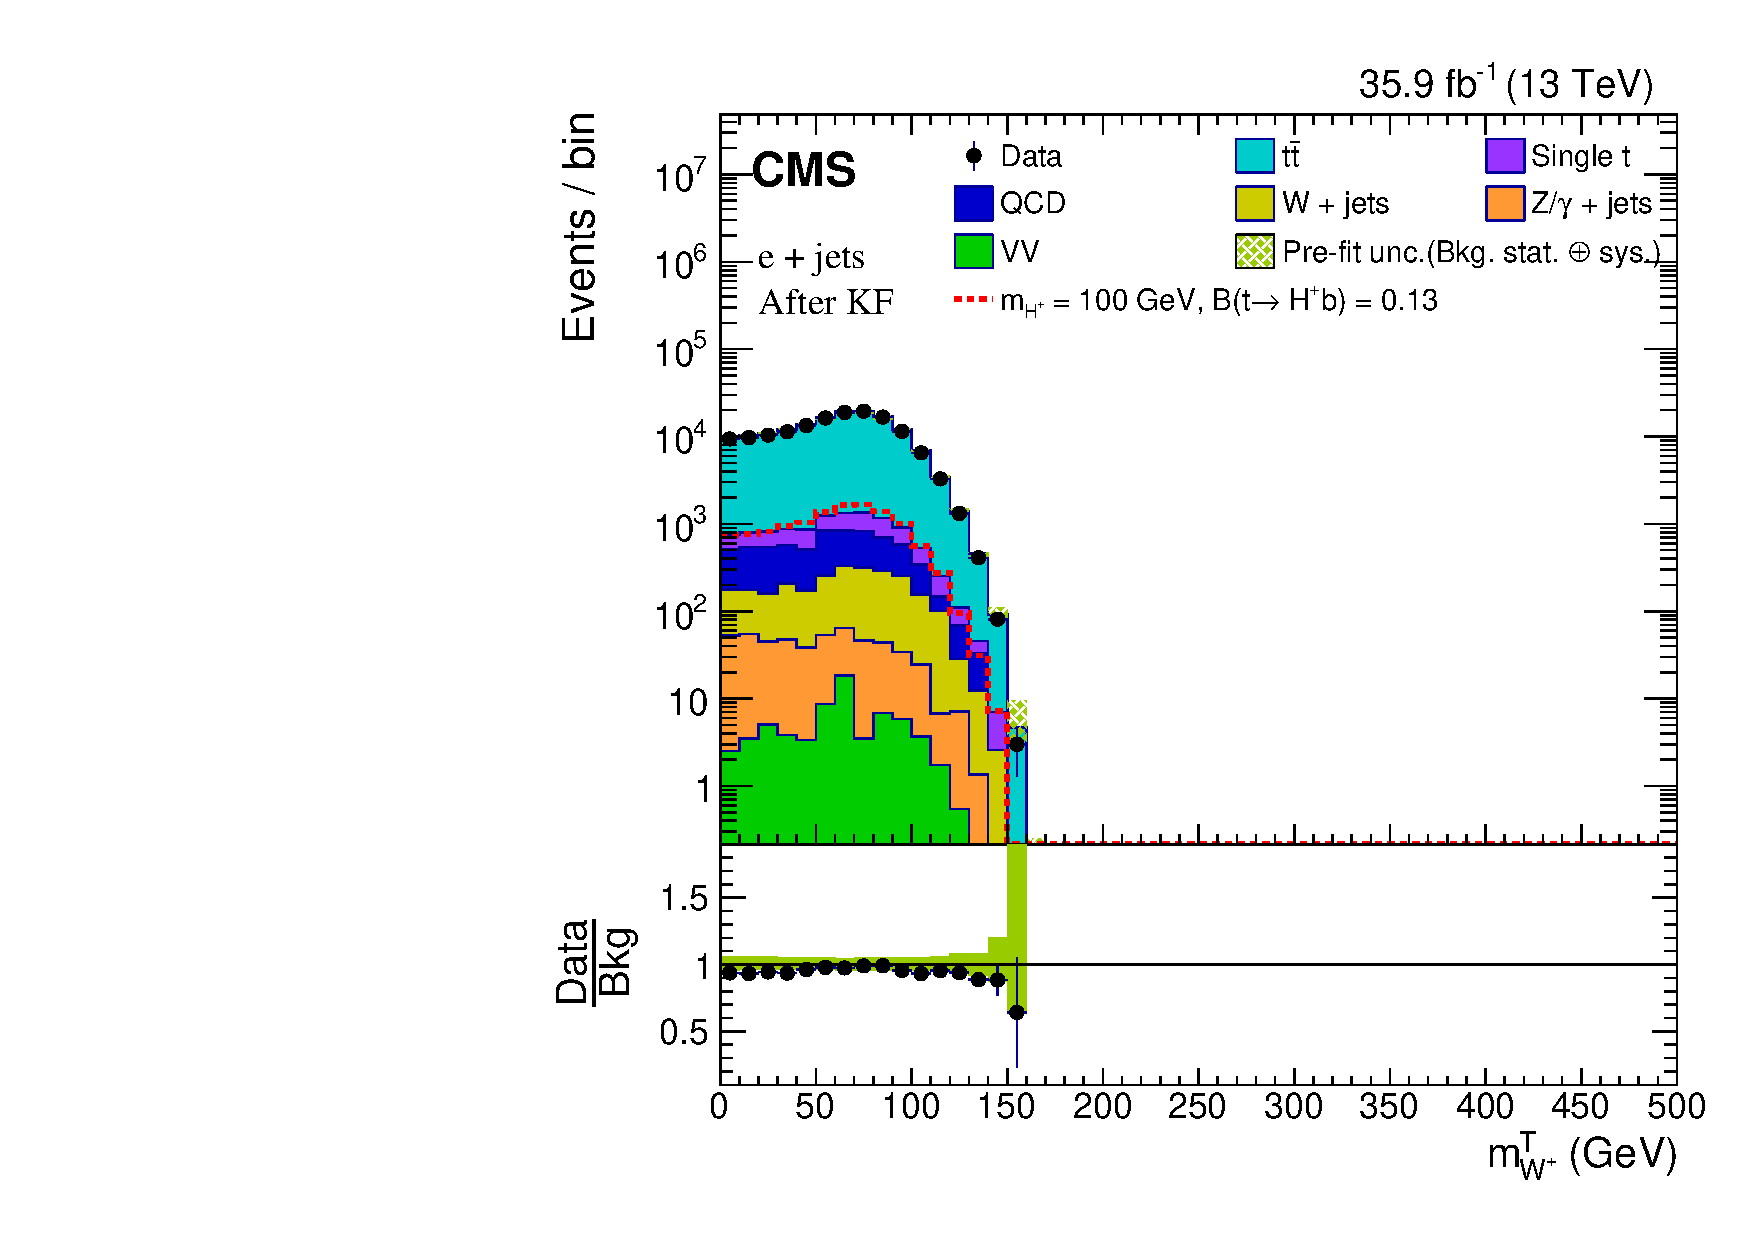
\includegraphics[width=0.45\linewidth]{Image/Electron/KinFit/wmt_eleKinFit.pdf}}
    \caption{Distribution of kinematic fitted $\MET$ and $m_{W^+}^{T}$ after kinematic fit selection as described
        in Sec.~\ref{s:secEvtSel}, for muons + jets and \ejets channel.}
    \label{fig:kfitPlot3}
\end{figure}
